
%%==================================================
%% demo.tex for BIT Thesis
%% modified by yang yating
%% version: 1.2
%% last update: Jan. 4th, 2018
%%==================================================

% 默认单面打印 oneside 、硕士论文模板 master

\documentclass[oneside, master]{BIT-thesis-grd}
\raggedbottom

% 模板选项: 硕士论文 master; 博士论文 doctor

%==============更改数学字体设置,Latin Modern Math 默认的的确有点细,看个人需要,下面提供一种方法,需要的可以取消注释=========%

%\usepackage[bold-style=ISO]{unicode-math} %采用unicode-math,可以直接输入Unicode公式,当然传统的输入就行
%\setmathfont{XITS Math}  %目前unicode-math 支持几种数学字体,具体用法可以查看帮助文档,这里采用类似times字体科学数学字体,可以取消注释对比
\usepackage{pifont}
\usepackage{array}
\usepackage{tikz}
\newcommand*{\mycircled}[1]{\lower.7ex\hbox{\tikz\draw (0pt, 0pt)%
		circle (.5em) node {\makebox[1em][c]{\small #1}};}}
	
\DeclareFontFamily{OT1}{cmrx}{}
\DeclareFontShape{OT1}{cmrx}{m}{n}{<->cmr10}{}
\let\saveLongrightarrow\Longrightarrow
\makeatletter
\renewcommand*{\Longrightarrow}{%
	\mathrel{\rlap{\fontfamily{cmrx}\fontencoding{OT1}\selectfont=}%
		\hphantom{\saveLongrightarrow}%
		\llap{$\m@th\Rightarrow$}}}
\makeatother

%\usepackage{extarrows}	 %数学箭头宏包
%\usepackage{latexsym,bm}        % 处理数学公式中和黑斜体的宏包
%\usepackage{amsmath,amssymb}    % AMSLaTeX宏包 用来排出更加漂亮的公式
%\makeatletter
%\renewcommand\normalsize{%
%	\abovedisplayskip 1\p@ \@plus1\p@ \@minus6\p@
%	\abovedisplayshortskip \z@ \@plus3\p@
%	\belowdisplayshortskip 3\p@ \@plus3\p@ \@minus3\p@
%	\belowdisplayskip \abovedisplayskip
%	\let\@listi\@listI}
%\makeatother

\begin{document}

%%%%%%%%%%%%%%%%%%%%%%%%%%%%%%
%% 封面
%%%%%%%%%%%%%%%%%%%%%%%%%%%%%%

% 中文封面内容(关注内容而不是表现形式)
\classification{\zihao{5} \setmainfont{Times New Roman} TP242.6}
\UDC{\zihao{5} \setmainfont{Times New Roman} 621.3}

\title{基于ROS的实时视觉/惯性/地磁等 \\ 多传感器融合定位系统研究}
\vtitle{基于 \rotatebox[origin=cc]{-90}{ROS} 的实时视觉惯性地磁等多传感器融合定位系统研究}

%\author{江正}
\author{}
%\institute{自动化学院}
\institute{}
%\advisor{李磊磊副研究员}
\advisor{}
%\chairman{陈家斌教授}
\chairman{}
\degree{工程硕士}
\major{控制工程}
%\school{北京理工大学}
\school{}
%\defenddate{2019年6月}
\defenddate{}

%\studentnumber{**********}


% 英文封面内容(关注内容而不是表现形式)
\englishtitle{Research on real-time vision/inertia/geomagnetic multi- \\ sensor fusion positioning system based on ROS}
%\englishauthor{Jiang Zheng}
\englishauthor{}
%\englishadvisor{A/Prof. Li Leilei}
%\englishchairman{Prof. Chen Jiabin}
\englishadvisor{}
\englishchairman{}
%\englishschool{Beijing Institute of Technology}
\englishschool{}
%\englishinstitute{School of Automation}
\englishinstitute{}
\englishdegree{Master of Engineering}
\englishmajor{Control Engineering}
%\englishdate{June,2019}
\englishdate{}

% 封面绘制
\maketitle

% 中文信息
\makeInfo

% 英文信息
\makeEnglishInfo

%打印竖排论文题目
\makeVerticalTitle

% 论文原创性声明和使用授权
\makeDeclareOriginal

%%%%%%%%%%%%%%%%%%%%%%%%%%%%%%
%% 前置部分
%%%%%%%%%%%%%%%%%%%%%%%%%%%%%%
\frontmatter

% 摘要
%%==================================================
%% abstract.tex for BIT Master Thesis
%% modified by yang yating
%% version: 0.1
%% last update: Dec 25th, 2016
%%==================================================

\begin{abstract}
视觉SLAM技术能够使机器人在未知的场景中,仅依靠相机进行定位和建图。然而单目视觉SLAM有众多的缺点,其中最显著的就是缺乏尺度信息,这使得纯粹的单目视觉SLAM无法在实际环境中使用。而IMU是一个在很多方面与相机互补的传感器,将IMU和单目视觉融合可构成一个具有绝对尺度的六自由度状态估计器。本文正是研究如何将视觉和IMU进行融合,获得高精度的状态估计。

本文首先对传感器进行数学建模与标定,使用高精度的工业级传感器搭建了一套独特的、简单的高精度硬件平台。然后针对硬件平台设计了多传感器融合算法,包括前端、初始化、后端和闭环。从前端提取图像的FAST特征,利用LK光流跟踪图像特征,预积分IMU数据。初始化将视觉与IMU对齐,得到状态估计的初始值。与其他初始化算法不同,本文研究的初始化算法能够在运动中实时初始化,并通过磁力计获得绝对的航向信息。后端采用一种基于紧耦合、非线性优化的方法,融合前端预积分的IMU数据和相机的特征观测数据。闭环采用词袋模型进行检测,并对检测到的闭环帧进行重定位,然后实施位姿优化,获得全局一致的定位轨迹。最后本文做了公开数据集实验和本地车载实验,并分析了每个实验的定位精度,验证了本系统硬件及软件算法的可行性和鲁棒性。

实验结果表明,本系统能够搭载在飞行器和汽车上,在室内或者室外进行高精度、鲁棒性的状态估计,从而对自身进行高精度的定位。


\keywords{视觉SLAM;惯性测量单元;视觉-惯性里程计;非线性优化 }
\end{abstract}

\begin{englishabstract}

   Visual SLAM technology enables the robot to locate and map in unknown scenes only depending on the camera. However, monocular visual SLAM has many disadvantages, the most significant of which is the lack of scale information, which makes the pure monocular visual SLAM unable to be used in the actual environment. The IMU is a sensor complementary to the camera in many aspects. The fusion of IMU and monocular vision can constitute a six-DoF state estimator with absolute scale. This paper is to study how to integrate vision and IMU to obtain high-precision state estimation.
   
   In this paper, the sensor is firstly modeled and calibrated, and a set of unique and simple high-precision hardware platform is built by using high-precision industrial-grade sensors. Then the multi-sensor fusion algorithm is designed for the hardware platform, including front end, initialization, back end and closed loop. FAST features of images were extracted from the front end, and LK optical flow was used to track image features, and pre-integration IMU data was obtained. The initialization aligns the vision with the IMU to obtain the initial value of the state estimation. Different from other initialization algorithms, the initialization algorithm studied in this paper can be initialized in real time in motion and obtain absolute yaw information through magnetometer. The back end adopts a method based on tight coupling and nonlinear optimization, and integrates the IMU data of the front end pre-integration with the feature observation data of the camera. The closed loop is detected by the word bag model, and the detected closed loop frame is repositioned, and then the pose optimization is carried out to obtain globally consistent positioning trajectory. Finally, this paper makes public data set experiment and local vehicle-mounted experiment, analyzes the positioning accuracy of each experiment, and verifies the feasibility and robustness of the system's hardware and software algorithm.
   
   Experimental results show that the system can be mounted on aircraft and vehicles, indoor or outdoor for high-precision, robust state estimation, so as to carry out high precision positioning of itself.
   

\englishkeywords{VSLAM;\quad IMU;\quad Visual–Inertial Odometry;\quad Nonlinear Optimization}

\end{englishabstract}

%% 符号对照表,可选,如不用可注释掉
%\begin{denotation}
	
\item[BIT] 北京理工大学的英文缩写
\item[\LaTeX] 一个很棒的排版系统
\item[\LaTeXe] 一个很棒的排版系统的最新稳定版
\item[\XeTeX] \LaTeX{}的好兄弟,事实上他有很多个兄弟,但是这个兄弟对各种语言的支持能力都很强
\item[ctex] 成套的中文\LaTeX{}解决方案,由一帮天才们开发
\item[\ce{H2SO4}] 硫酸
\item[$ e^{\pi{}i}+1=0$] 一个集自然界五大常数一体的炫酷方程
\item[\ce{2H2 + O2 -> 2H2O}] 一个昂贵的生成生命之源的方程式

\end{denotation}

% 加入目录
\tableofcontents


%加入图、表索引(同时取消图表索引中章之间的垂直间隔)
%\let\origaddvspace\addvspace
%\renewcommand{\addvspace}[1]{}
%\listoffigures
%\listoftables
%\renewcommand{\addvspace}[1]{\origaddvspace{#1}}



%%%%%%%%%%%%%%%%%%%%%%%%%%%%%%
%% 正主体部分
%%%%%%%%%%%%%%%%%%%%%%%%%%%%%%
\mainmatter

%% 各章正文内容
%%==================================================
%% chapter01.tex for BIT Master Thesis
%% modified by yang yating
%% version: 0.1
%% last update: Dec 25th, 2016
%%==================================================
\chapter{绪论}
\label{chap:intro}
\section{研究背景及意义}

科学技术总是能让我们生活变得更加美好,它的发展经常在我们的意料之外,特别是机器人这个行业,在过去几十年里发展迅速。银行大厅里可爱的机器人助手、现代化餐厅的送餐机器人、室内清扫机器人、儿童手中的无人机玩具等,这些移动机器人都是现代机器人技术发展的结晶。世界上很多研究机构,例如波士顿公司和MTI等,正在研究仿生机器人,并且取得了显著的成果。随着人工智能和5G技术的快速发展,机器人行业的一个分支——无人驾驶技术,正成为国际上一个重要的研究方向和热点。所有这些机器人都有一个共同点——自主性,拥有在不熟悉的环境中移动而不依赖外部信息和控制的能力。自主定位与导航技术为实现这一共性提供了基础。

SLAM是Simultaneous Localization and Mapping的缩写,译为“同时定位与地图构建”\upcite{Zhaopeng2015}。它是指携带有特定传感器的移动载体,在未知的陌生环境下,边运动边感知周围环境,并构建地图,同时估计出本体在地图中的位置\upcite{davison2007monoslam}。大多数机器人实现自主定位用的都是SLAM技术。SLAM可以使用激光传感器,称为激光SLAM。也可以使用视觉传感器,称为视觉SLAM,简称VSLAM(Visual SLAM)。早期研究者大都以激光SLAM研究为主,现今,随着计算机硬件和软件的极速发展,视觉SLAM凭借着信息量大、体积小、重量轻、适用范围广和成本低等优点受到广泛关注,逐渐成为研究者心中的热门研究领域。

然而视觉SLAM本身也存在着诸多问题,比如当相机运动过快时图像出现模糊或者前后两帧没有重叠区域导致特征匹配失败,无法应对特征缺失和大面积重复纹理场景,光照变化幅度大时跟踪容易失败等等。惯性测量单元(Inertial Measurement Unit,IMU)输出频率高,在短时间内对快速运动估计较为准确。大多数IMU读数漂移严重,而相机的漂移较小。相机属于外感受型传感器,当图像变化时我们无法知道是相机在运动还是周围环境发生了变化,所以纯视觉SLAM常常难以应对动态场景。而IMU属于内感受型器,能够感受到自身的6-DoF(六自由度)运动信息。因此相机和IMU被认为是一对具有互补性的传感器。在大多数情况下,最好的状态估计就是同时有效利用内感受型和外感受型传感器的观测值\upcite{barfoot2017state}。因此视觉/惯性融合成为目前学术界的研究热点。

%  1.2
\section{国内外研究现状}
%\label{sec:***} 可标注label
SLAM技术已经有30多年的历史了,伴随着计算机硬件的巨大改进,研究热点从激光转移到视觉。有部分研究者提出了划时代的理论算法,为SLAM的发展奠定了理论基础。还有部分研究者实际研究并编程实现了SLAM的各种算法的完整框架,甚至开源了他们的源代码,为SLAM的发展做出了无私的贡献。正是因为有很多这样孜孜不倦、无私奉献的学者,SLAM技术才能日渐成熟,走向大众。

下面,本文将首先对视觉SLAM的发展历程和有影响力的研究成果经行概述,然后对视觉/惯性融合的发展现状经行详细阐述。

%  1.2.1
\subsection{视觉SLAM研究概述}
%\label{sec:features}

SLAM最早叫做概率SLAM(probabilistic SLAM)。早期大多以激光传感器为主,SLAM中存在一个基本问题——全局一致性。Cheesman\upcite{smith1986representation}和Durrant-Whyte\upcite{durrant1988uncertain}为了描述路标与路标之间的相互关系而建立了一个统计学框架,该框架主要用来解决几何上的不确定性。他们证明了估计的路标位置之间具有强关联性,并且这种关联性会随着观测的时间增加而增加。

%6
Ayache和Faugeras最先从事视觉SLAM的研究。Smith等人提出移动机器人在陌生环境中获取的路标时,因为这些路标具有相同的估计误差,所以路标的估计值也是相关的\upcite{smith1990estimating}。这样就加大了难度。因为状态向量中将包含机器人的位姿和每一个路标点的观测值,而且每观测一次都要实时更新,这导致状态向量的维数非常大,进而带来巨大的计算量。SLAM中的地图有一个收敛的性质,因为Smith等人将其忽略,并假设地图的估计误差是发散的,因此学者们只能视路标点之间没有相关性或者相关性很小。这是因为这个原因,当时的SLAM大都是将定位和建图问题分开处理的。

%[7][8]

1995年文章International Symposium on Robotics提出了收敛性和同时定位建图的概念\upcite{durrant1996localization},此时研究者们才将定位与地图构建问题结合在一起,突破了新的理论。之后SLAM的研究集中在计算速度的提升以及多源信息融合上。在ISRR99上,Thrun首次提出将基于卡尔曼滤波(Kalman filter)的SLAM与概率定位建图相结合\upcite{thrun1998probabilistic}。

进入二十一世纪后,因为计算机硬件性能的提升,研究热潮逐渐转向以相机为传感器的视觉SLAM,并出现了很多可以实现的理论框架,甚至有一些理论框架已经落地市场化。

%[9][10][11]

A. J. Davison可以说是视觉SLAM领域中的领头人,他在单目视觉SLAM中做了奠基性的工作\upcite{davison2007monoslam}\upcite{Davison03real-timesimultaneous},极大的推动了视觉SLAM的发展。他在2007年的一篇文章中提出了MonoSLAM\upcite{davison2007monoslam},该系统有一个重大突破——可以实时运行。MonoSLAM仅仅依靠单目相机,检测每一帧图像中的Shi-Tomasi角点\upcite{Shi94goodfeatures},该角点是很稀疏的角点,然后在投影椭圆中实施特征匹配。经典的扩展卡尔曼滤波器(EKF)被用于SLAM后端,路标点的位置被建模为高斯分布,位姿及其关联的路标点构成状态向量,并实时更新其均值和协方差。

%[11][12]

Klein等人在2007年提出并开源了PTAM(Parallel Tracking and Mapping)\upcite{klein2007parallel},并在两年后将PTAM算法移植到智能手机上\upcite{klein2009parallel}。PTAM首次提出并编程实现了前端特征跟踪和后端建图的并行化,将前端和后端分开来并行计算,这是一个值得称赞的突破。时至今日,这种思想仍在继续使用,效果极好。此外,PTAM还创新地使用了关键帧机制,这一重大创新使得处理器不必处理每一帧图像,而是处理几个关键的图像,大大减少了计算量。而且,对比MonoSLAM,PTAM在后端不使用卡尔曼滤波器。取而代之的是非线性优化,这在历史上是第一次的。这一开创性突破直接导致了在PTAM之后,研究者开始以非线性优化为主来设计后端算法。并采取关键帧机制和多线程并行化思想。PTAM对视觉SLAM研究提出了很多创新的算法和重大革新,对视觉SLAM的发展做出了巨大的贡献。

%[13][14][15]

Raul Mur-Artal等人在2015年提出了ORB-SLAM系统\upcite{mur2015orb}。如果说MonoSLAM和PTAM是在时间上距离我们较为久远的方案,那么ORB-SLAM则是距离我们很近的全新的方案。ORB-SLAM是自2015年以来所有纯视觉SLAM算法中最为优秀的算法之一。ORB-SLAM提出了自己独特的创新和改进,抛弃了传统的SIFT(Scale Invariant Feature transform)\upcite{lowe2004distinctive}和SURF(Speeded Up Robust Features)\upcite{bay2008speeded}特征,采用自己独特的ORB特征进行特征提取。相比于SIFT和SURF,ORB特征计算快,可以在处理器上实现实时计算。与Harris角点相比,ORB特征点比Harris角点多了一个尺度不变特性以及描述子,可以快速的进行特征匹配、回环检测或者重定位。因此,ORB特征是一种折衷了计算速度和计算精度的优秀特征方案。在回环检测中ORB-SLAM使用了ORB字典,大大减少了系统的累计误差,同时在特征丢失之后也能快速找回,大大提高了整个系统的鲁棒性。最后,该系统创新地使用了三线程并行方案。使得前端、后端和回环各自有条不紊的工作。ORB-SLAM是主流特征点法的巅峰之作,极大的推动了视觉SLAM技术的发展。

MonoSLAM、PTAM和ORB-SLAM的运行效果如图\ref{fig1_1}所示。

\begin{figure}[h]\setlength{\belowcaptionskip}{-12pt}
	\centering
	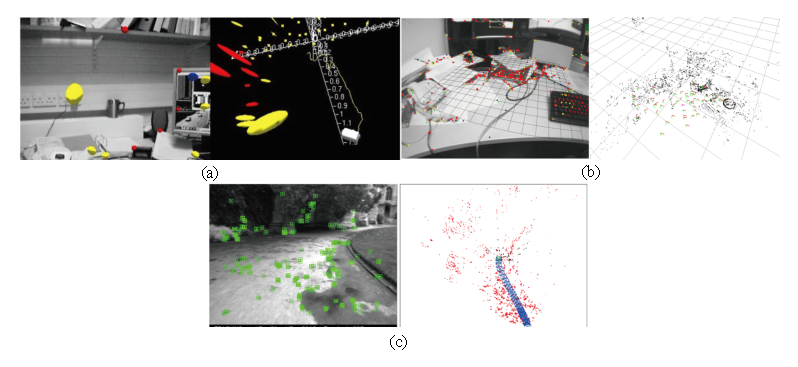
\includegraphics[width=0.75\textwidth]{figures/chapter1/fig1_1}
	\caption{(a) MonoSLAM;(b) PTAM;(c) ORB-SLAM.}\label{fig1_1}
\end{figure}

以上所介绍的视觉SLAM系统都是基于特征点的方案,称作特征点法或者间接法。特征点是人为从图像中提取和设计的特殊的角点,一般包括关键点和描述子。在视觉SLAM的前端跟踪中用来代替整张图片的纹理,在后端中将其视为路标点进行迭代优化。特征点的存在使得相机在运动的过程中,SLAM系统前端跟踪也能取得良好的效果。万事有利必有弊,虽然特征点法应用广泛,鲁棒性高,但是特征点法仍然有缺点:提取关键点需要花费很长时间;提取特征点意味着主动丢掉了图像中的其他信息;在一些单色无纹理区域,往往很难提取特征点,在重复纹理区域,特征点普遍跟踪混乱,无法使用。

除了特征点法,近几年来研究者们也在研究一种基于像素的直接法。直接法与光流法非常相似,其灰度不变性的假设是应用的前提。该方法不需要提取图像特征点,而是通过最小化亮度误差直接估计像素深度,从而计算像素3D空间位置和相机的运动。因此,直接法相比于特征点法在计算速度上有很大提升,并且能适应特征缺失和图像模糊的场景。同时,直接法仅用CPU就能构建稀疏或者半稠密地图,这是特征法做不到的。


%[16][17]
2014年,TUM计算机视觉组的J. Engel 等人提出LSD-SLAM\upcite{engel2014lsd}\upcite{engel2013semi},LSD-SLAM采用直接法,可以构建半密集三维地图。这是单目直接法在视觉SLAM中的典型应用。与以往的方案不同,LSD-SLAM仅使用CPU就可以完成半密集地图的三维重建。LSD-SLAM有很多自己的创新之处,例如,LSD-SLAM既不是利用像素,也不是利用块匹配去跟踪图相机,而是在极线上等间距的取五个点,计算其SSD(Sum of Squared Distance);LSD-SLAM没有复杂的初始化过程,而是对深度随机赋值,然后在将计算出来的深度归一化,得到全局一致的尺度;使用光度不确定性项来计算深度协方差;使用李群和李代数 来对关键帧进行约束,在后端优化中考虑不同的尺度,进而减小大范围场景中的尺度漂移现象。

%[18]
Forster 等人在2014年提出SVO(Semi-direct Visual Odoemtry)\upcite{forster2014svo}。SVO采用稀疏直接法,也称作“半直接法”。之所以成为“半直接法”,是因为SVO同时使用了特征点法和直接法,在前端提取角点,然后利用角点周围的信息通过直接法估计出相机的运动以及自身的位置。该方案对比于其他方案,显著的优势是速度极快,它甚至可以在低端处理器上实现实时计算,这使得SVO可以应用到无人机、智能手机、VR等设备上。另外,SVO在理论上也有一个重大的创新,提出了深度滤波器的概念。在估计角点的位置时,逆深度被用来设计参数,使之能够更好的计算特征点位置。

LSD-SLAM和SVO的运行效果如图\ref{fig1_2}所示。

\begin{figure}[h]\setlength{\belowcaptionskip}{-12pt}
	\centering
	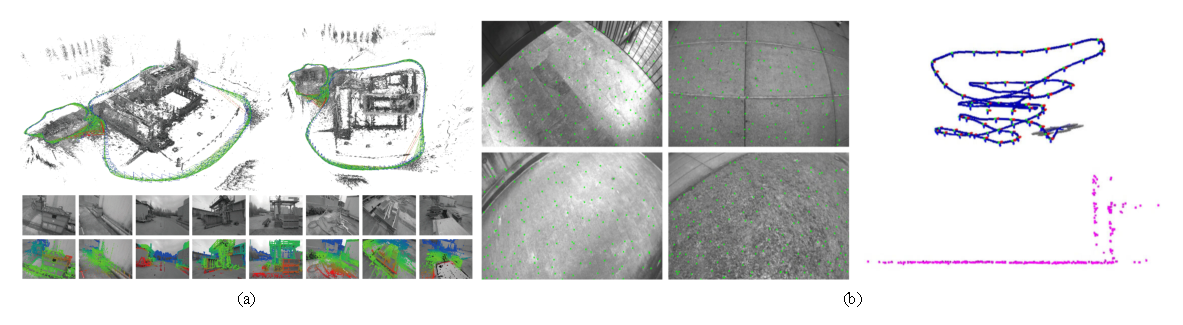
\includegraphics[width=0.75\textwidth]{figures/chapter1/fig1_2}
	\caption{(a) LSD-SLAM;(b) SVO.}\label{fig1_2}
\end{figure}

%[19][20][21][22][23][24][25][26][27]
国内SLAM的研究因为起步较晚,所以一直落后于国外,但是,近几年来随着自动驾驶行业的发展,SLAM研究越来越受到重视。很多高校都在开展SLAM相关的课题研究,也出现了一些详细解读SLAM技术的文章\upcite{权美香2016视觉}\upcite{刘浩敏2016基于单目视觉的同时定位与地图构建方法综述}\upcite{何俊学2010基于视觉的同时定位与地图构建方法综述}。上海交通大学的邹丹平等人提出了基于线特征的StructSLAM\upcite{zhou2015structslam}以及基于多目相机的Co-SLAM\upcite{zou2013coslam}。浙江大学计算机学院的章国锋等人于2013年提出了RDSLAM\upcite{tan2013robust},RDSLAM的创新之处是将传统的随机采样一致性(RANSAC)\upcite{fischler1981random}算法改为一种基于时间序列和先验信息的自适应RANSAC算法,该算法弥补了之前算法在动态场景下表现欠佳的缺点。2016年,他们又提出了改进版的基于移动设备的RKSLAM\upcite{liu2016robust},可以实时运行。2017年,他们提出基于RGB-D相机的RKD-SLAM系统\upcite{liu2017robustRGB},RKD-SLAM能够构建稠密地图。

%1.2.2
\subsection{视觉/惯性融合研究概述}
%\label{sec:requirements}

尽管仅用相机就能完成定位和建图任务的视觉SLAM。然而,纯视觉SLAM往往因为各种各样的问题导致其应用场景有限,鲁棒性低。广大学者和工程师往往希望算法能够得到实际的应用,而不是局限于在个人PC上跑demo。在这种应用需求的背景下,视觉与惯性融合的定位方案逐渐成为学术界的研究热点。

%[28]
目前的VIO算法可以分为松耦合和紧耦合\upcite{martinelli2014closed}。松耦合将相机和IMU分开处理,各自单独估计,然后将二者估计出的结果进行融合。紧耦合是指将IMU和相机的状态量融合在一起,组成一个整体的状态方程。然后对状态方程进行求解。类比于纯视觉SLAM,VIO也可以分为基于滤波和基于优化两大类。下面将基于这几种分类对VIO的研究现状进行分析。

%[29][30][31]
宾夕法尼亚大学Kumar实验室的Mourikis等人于2007年提出基于滤波的紧耦合VIO方案——MSCKF(Multi-State Constraint KF)\upcite{mourikis2007multi},并于2015年提出了改进的MSCKF\upcite{li2013high}。传统的EKF-SLAM(Extended kalman filtering SLAM)\upcite{bloesch2015robust}系统会将图像的特征信息加入到状态向量和协方差矩阵里,如果在初始化特征点深度和协方差矩阵的时候有误差,那么很容易造成全局轨迹不一致的情况。而MSCKF始终保持一个先进先出的滑动窗口序列,在滑窗内建立EKF的预测和更新。

%[32]
苏黎世联邦理工学院自动控制系统实验室的Stephen Weiss等人于2013年提出基于滤波的松耦合VIO方案——SSF和MSF\upcite{lynen2013robust}。松耦合系统没有紧耦合系统那么繁杂,而且MSF可以用来融合除相机和IMU之外的其他多种传感器。松耦合还有另一个优点:当一个传感器不能工作时,系统任然能够依靠其他传感器正常运行。紧耦合系统则是所有传感器相互依赖,缺一不可。

%[33][34]
2014年,苏黎世联邦理工学院的Stefan Leutenegger等人提出基于优化的紧耦合VIO方案——OKVIS\upcite{Leutenegger_keyframe-basedvisual-inertial}。OKVIS在一个滑窗内优化关键帧,带权重的视觉重投影误差和带权重的IMU误差组成残差项。前端提取尺度不变的Harris特征点,并计算BRISK描述子\upcite{leutenegger2011brisk},后端使用非线性优化的方式进行状态估计。另外OKVIS同时支持单目和双目两种类型的相机,Leutenegger的实验表明在双目情况下有更好的效果。

%[35][31]
2015年,苏黎世联邦理工学院的Michael Bloesch等人提出了基于滤波的紧耦合VIO方案——ROVIO\upcite{bloesch2015robust}。ROVIO利用EKF进行状态估计,而且有许多创新的地方。首先,ROVIO在提取角点时采用的是FAST角点\upcite{smith2002fast},使用矢量坐标点方向,用标量表示坐标点大小;其次,图像块用于描述所有的角点,视频流用于多级表达;最后使用惯导计算出的位姿估计视觉重投影的光度误差,并将其用于后端优化。ROVIO仅仅支持单目相机。

%[36]
2017年,香港科技大学的沈绍杰等人提出基于优化的紧耦合VIO方案——VINS-Mono\upcite{qin2018vins}。VINS-Mono是一个基于滑动窗口的紧耦合非线性优化系统。在初始化阶段,通过松耦合的方式融合相机和IMU,从而获得位置、姿态和尺度的初始值。在后端通过IMU残差、视觉残差和边缘化残差构成目标函数,用非线性优化进行计算状态量。值得注意的是,VINS-Mono还具有回环检测和重定位的功能,并在检测到回环时进行4-DoF全局位姿图优化。VINS-Mono在精度和鲁棒性上都表现优异,是一个极具实用价值的VIO开源方案。

%[37]
基于优化的松耦合方案不多,因为学术界普遍认为其效果没有紧耦合好。2016年,Gabe Sibley等人在其文章中提到了基于优化的松耦合方法\upcite{falquez2016inertial}。简而言之,就是将前端计算出的位姿进行坐标变换,然后放到IMU的优化框架中。

目前,VIO算法已经应用在包括自动驾驶、飞行机器人和VR/AR等领域。视觉/惯性融合方案总结如图1.3。本文将对基于优化的紧耦合VIO方案进行细致的研究,并基于单目相机、IMU和磁力计实际搭建一套高精度、简单易用的视觉/惯性/地磁等多传感器融合定位系统。

\begin{figure}[h]\setlength{\belowcaptionskip}{-12pt}
	\centering
	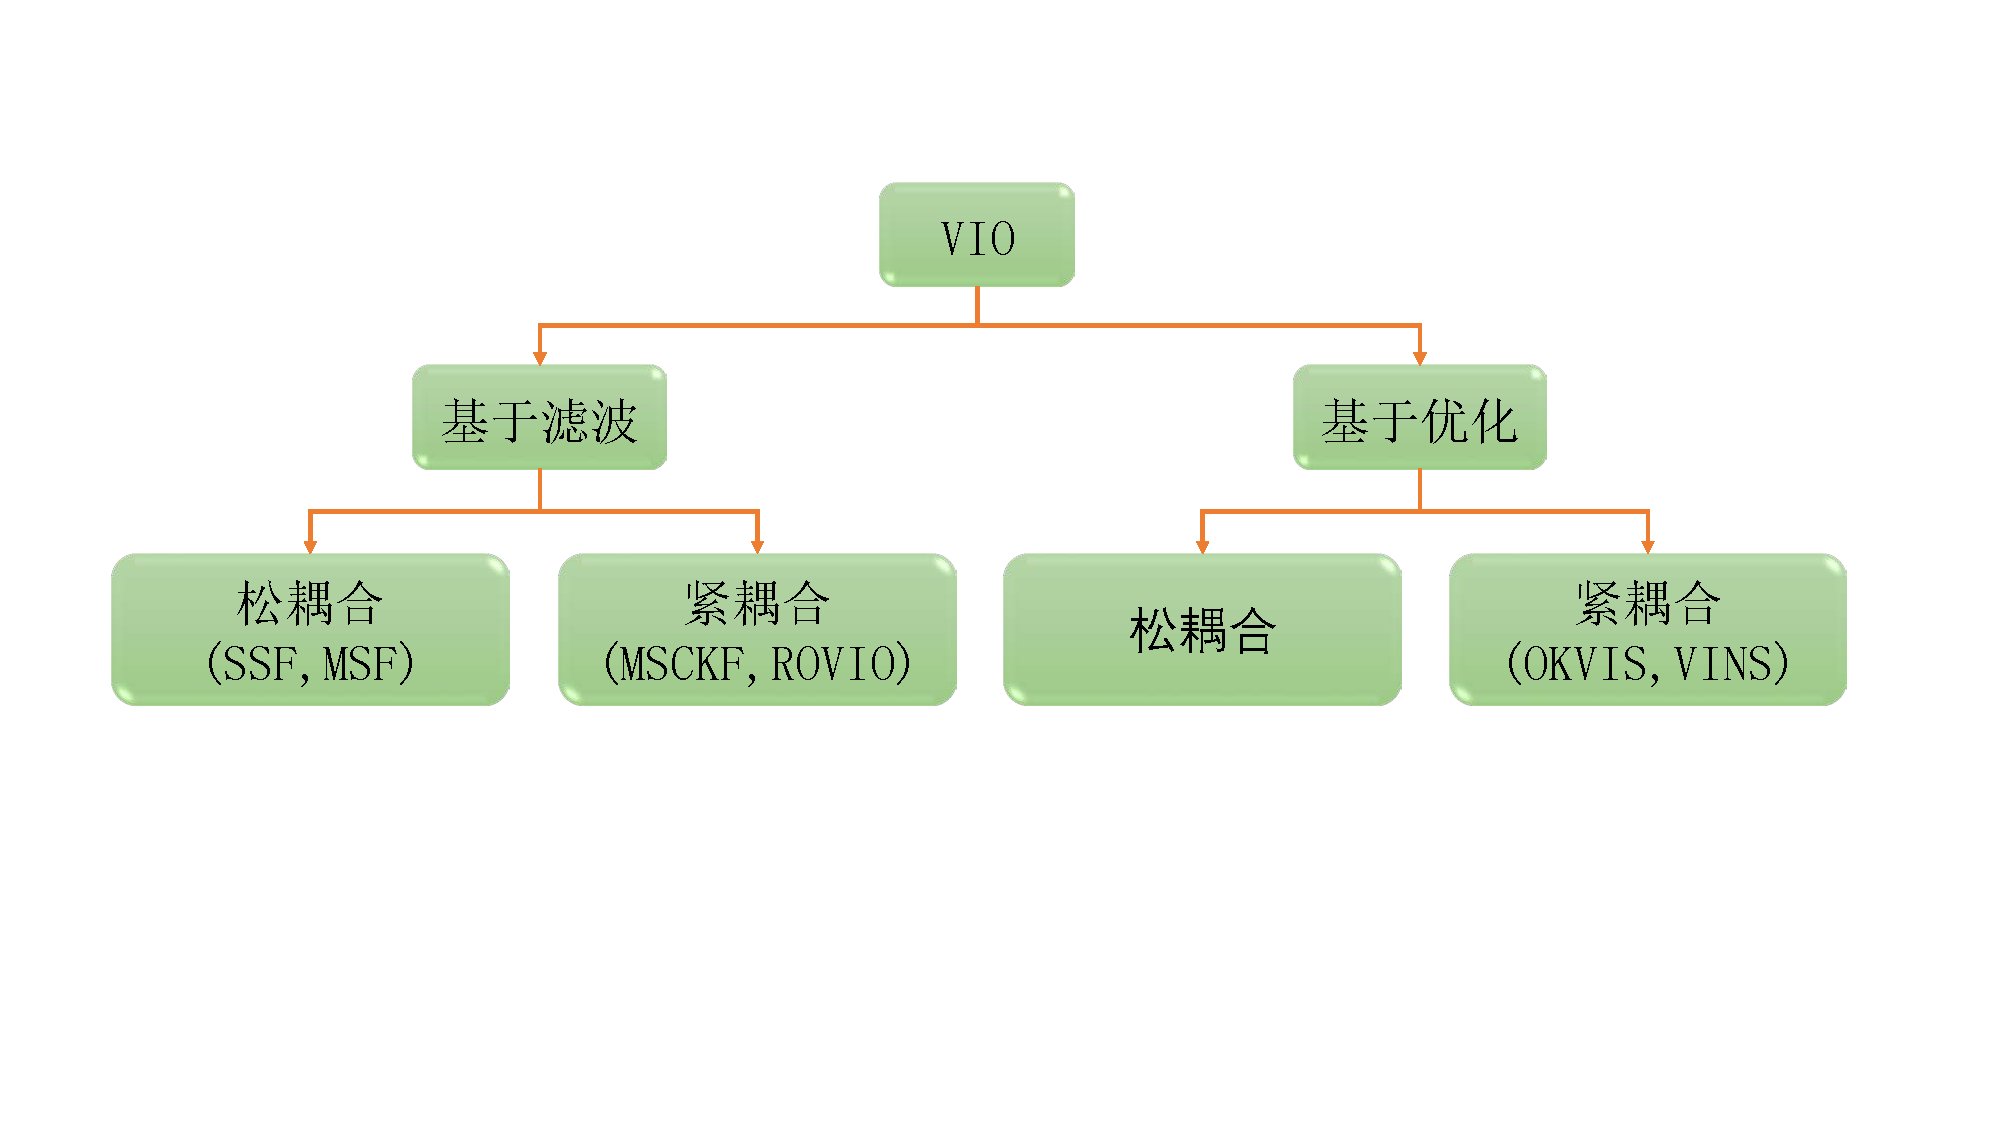
\includegraphics[width=0.75\textwidth]{figures/chapter1/fig1_3}
	\caption{(a) LSD-SLAM;(b) SVO.}\label{fig1_3}
\end{figure}

%  1.3
\section{本文主要工作及结构安排}

本文以视觉/惯性融合为主,磁力计为辅,研究多传感器融合定位算法,并实际搭建一套软硬件结合的多传感器融合定位系统。

本文主要工作如下:

(1)	搜集并研读国内外视觉SLAM和VIO相关的论文,详细阐述了视觉SLAM和VIO的国内外发展现状;

(2)	与市场上普通的消费级视惯套件不同,本文对高精度的工业级传感器进行硬件同步,搭建了一套高精度的多传感器融合定位系统硬件平台;

(3)	研究了视觉SLAM算法、多传感器融合算法,针对自己的硬件系统设计前端、后端及闭环算法,并创新的实现了运动中在线实时初始化和绝对航向初始化;

(4)	在ROS下编程实现所有算法,整个系统拥有良好的可视化功能,可扩展性强;

(5) 进行公开数据集实验和本地实验,分析了系统在不同环境下的定位精度,验证了系统的可行性。

本文各个章节安排如下:

第二章主要研究了系统的硬件平台。首先研究了传感器(相机和IMU)的数学模型及选型;然后研究传感器的标定以及硬件同步原理;最后研究了基于ROS的传感器信息采集方法。

第三章主要研究系统的前端和初始化算法。首先研究视觉信息预处理算法;然后研究IMU预积分原理;最后研究了系统初始化流程,包括纯视觉初始化和视觉/惯性联合初始化。

第四章主要研究系统后端和闭环算法。首先研究了后端非线性优化的方法;然后研究了闭环检测算法;最后研究了重定位和闭环优化算法。

第五章主要是实验。验证算法有效性,并分析定位误差。包括公共数据集实验和本地校园环境实验。


\chapter{硬件平台搭建}
\label{chap:2}
本章主要研究硬件平台的构成及各个传感器数学模型,为后续章节研究VIO算法提供硬件支撑。首先,研究传感器的数学模型以及选型;其次,研究传感器的标定原理及方法,传感器之间的硬件同步方案;最后,研究传感器信息采集方案。
\section{传感器模型与选型}
\subsection{相机及畸变模型}
\label{chap:2.1.1}
(1)针孔相机模型

众所周知,小孔成像能够将3D物体投影成2D图像。相机成像原理类似,称为针孔相机模型。如图\ref{fig2_1}所示。
\begin{figure}[h]\setlength{\belowcaptionskip}{-12pt}
	\centering
	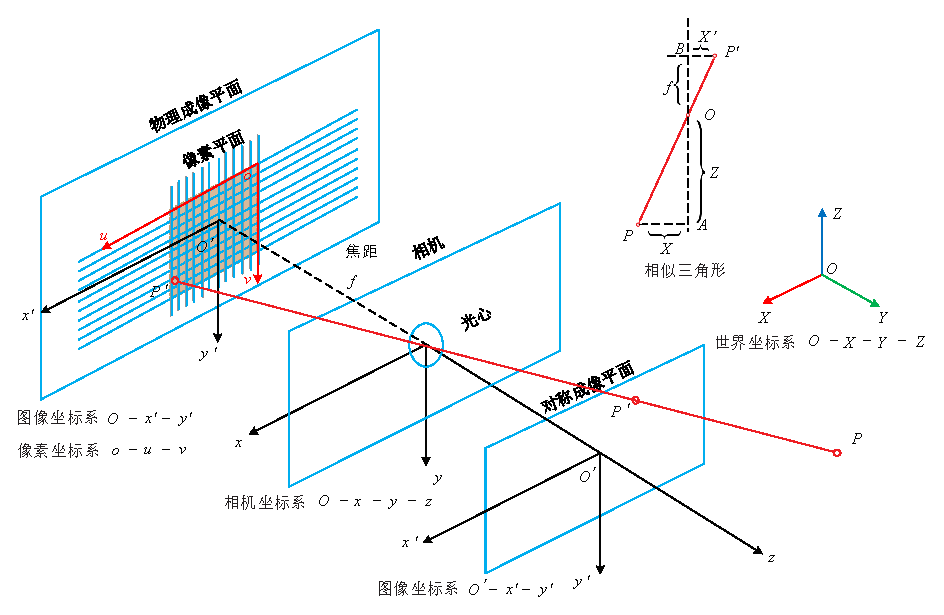
\includegraphics[width=1\textwidth]{figures/chapter2/fig2_1}
	\caption{针孔相机模型}\label{fig2_1}
\end{figure}
其中$O-x-y-z $是相机的坐标系,$z $轴正方向是相机前方,向右为$x $轴正方向,向下为$y $轴正方向。$O $为相机的光心,即针孔模型的针孔。真实世界中三维坐标点$P$,经过光心$O $投影到物理成像平面$O^{\prime}-x^{\prime}-y^{\prime}$上,即图像坐标系,投影坐标点是$P^{\prime} $。设$P$在相机坐标系下的坐标为$[X, Y, Z]^{T} $,$P^{\prime} $ 在图像坐标系下的坐标为$[X^{\prime}, Y^{\prime}]^{T} $ ,光心到物理成像平面的距离为焦距$f$ 。那么,根据相似三角形可得:
\begin{equation}
\label{eqn:2.1}
	\frac{Z}{f}=-\frac{X}{X^{\prime}}=-\frac{Y}{Y^{\prime}}
\end{equation}
其中的负号是因为这个成像看起来是上下颠倒的。为了简化模型,将物理成像平面对称平移到相机的前方,即与三维空间点 $P$ 在同一侧。

这个时候就可以将式(\ref{eqn:2.1})中的负号去掉,得到更加简洁的式子:
\begin{equation}
\label{eqn:2.2}
	\frac{Z}{f}=\frac{X}{X^{\prime}}=\frac{Y}{Y^{\prime}}
\end{equation}
整理得到:
\begin{equation}
\label{eqn:2.3}
	\left\{\begin{aligned} X^{\prime} &=f \frac{X}{Z} \\ Y^{\prime} &=f \frac{Y}{Z} \end{aligned}\right.	
\end{equation}
将成像平面平移到相机前方只是为了简化成像模型,是一种数学手段,不会带来负面影响。所以,在不引起异议的情况下,将这种简化的成像模型定义为针孔模型。

式(\ref{eqn:2.3})建立了三维空间点 和它的二维成像点 之间的映射关系。然而,相机采集的图像是以像素为单位的,所以,为了描述光线到像素之间的映射关系,假设在物理成像平面上固连了一个像素平面 ,如图\ref{fig2_1}所示。

图像的左上角$o $是像素坐标系的原点,向右为$u $轴正方向,向下为$v $轴正方向。设$P^{\prime} $在像素坐标系下的坐标为$[u, v]^{T} $ ,像素坐标在$u $轴上缩放了$\alpha $倍,在$v $轴上缩放了$\beta $倍,原点平移了$\left[c_{x}, c_{y}\right]^{T} $。那么,$P^{\prime} $的图像坐标与像素坐标之间的映射关系为:
\begin{equation}
\label{eqn:2.4}
\left\{\begin{array}{l}{u=\alpha X^{\prime}+c_{x}} \\ {v=\beta Y^{\prime}+c_{y}}\end{array}\right.
\end{equation}
代入式(\ref{eqn:2.3}),得:
\begin{equation}
\label{eqn:2.5}
\left\{\begin{array}{l}{u=f_{x} \frac{X}{Z}+c_{x}} \\ {v=f_{y} \frac{Y}{Z}+c_{y}}\end{array}\right.
\end{equation}
其中,$f_x=\alpha f$ ,$f_y=\beta f  $ 。 $f $ 的单位为米,$\alpha ,\beta $ 得单位为像素每米,$f_x $  和 $f_y $  的单位为像素。通过齐次坐标,将式写成矩阵形式,得:
\begin{equation}
\label{eqn:2.6}
\left( 
\begin{array}{l}{u} \\ {v} \\ {1}\end{array}
\right)=
\frac{1}{Z} \left( 
\begin{array}{ccc}{f_{x}} & {0} & {c_{x}} \\ {0} & {f_{y}} & {c_{y}} \\ {0} & {0} & {1}\end{array}
\right) 
\left( 
\begin{array}{l}{X} \\ {Y} \\ {z}\end{array}
\right) 
\triangleq \frac{1}{Z} \bm{K} \bm{P}
\end{equation}
等式两边同时乘以$Z $得:
\begin{equation}\label{eqn:2.7}
Z \left( \begin{array}{l}{u} \\ {v} \\ {1}\end{array}\right)=\left( \begin{array}{ccc}{f_{x}} & {0} & {c_{x}} \\ {0} & {f_{y}} & {c_{y}} \\ {0} & {0} & {1}\end{array}\right) \left( \begin{array}{l}{X} \\ {Y} \\ {Z}\end{array}\right) \triangleq \bm{K} \bm{P}
\end{equation}
其中,$\bm{K} $ 为相机的内参矩阵,下文中的相机标定需要标定此参数。有时候,为了不失一般性,可以在内参矩阵中添加一个扭曲参数 $\gamma $ ,该参数用来表示像素坐标系的两个坐标轴之间的扭曲程度。此时,内参矩阵$\bm{K} $有5个参数:
\begin{equation}
\label{eqn:2.8}
\bm{K} = \left[\begin{array}{ccc}f_x&\gamma&c_x\\0&f_y&c_y\\0&0&1\end{array}\right]
\end{equation}

值得注意的是,式(\ref{eqn:2.6})中$\bm{P} $ 是点$P $ 在相机坐标系下的坐标。记点$P $在世界坐标系下的坐标为 $\bm{P}_w $ ,则  $\bm{P} $ 和  $\bm{P}_w $ 之间存在一个坐标变换,这个变换矩阵由相机当前的位姿决定。记点$P $在像素坐标系下的坐标为$\bm{P}_{uv} $ ,设相机的旋转和平移为 $\bm{R} $ ,$\bm{t} $ ,那么有:
\begin{equation}
\label{eqn:2.9}
Z \bm{P}_{u v}=Z \left[ \begin{array}{l}{u} \\ {v} \\ {1}\end{array}\right]
=\bm{K}\left(\bm{R} \bm{P}_{w}+\bm{t}\right)=\bm{K} \bm{T} \bm{P}_{w}
\end{equation}
其中,$\bm{T} $为变换矩阵,又叫做特殊欧式群(Special Euclidean Group):
\begin{equation}
\label{eqn:2.10}
S E(3)=\left\{
\bm{T}=\left[ \begin{array}{cc}{\bm{R}} & {\bm{t}} \\ {\bm{0}^{T}} & {1}\end{array}\right] \in \mathbb{R}^{4 \times 4} | 
\bm{R} \in S O(3), \bm{t} \in \mathbb{R}^{3}\right\} 
\end{equation}

式(\ref{eqn:2.9})两侧使用的都是齐次坐标,也就是对相机投影平面进行了归一化,所以式(\ref{eqn:2.9})可以简化为:
\begin{equation}
\label{eqn:2.11}
\boldsymbol{P}_{u v}=\boldsymbol{K} \boldsymbol{T} \boldsymbol{P}_{w}
\end{equation}

式(\ref{eqn:2.11})表达了世界坐标系下的坐标与像素坐标系下的坐标之间的映射关系,也就是所谓的针孔相机模型。

(2)相机畸变模型

上一小节研究的针孔相机模型是理想情况下的模型,实际上,相机的镜头影响光线的传播方向,进而影响成像。影响分为两个方面:一是镜头的形状会对光线产生折射,二是镜头和相机在机械组装时镜头和感光平面不完全平行导致成像的位置发生变化。这两种影响都会使图形产生畸变,前者引起的畸变称为径向畸变,后者引起的畸变称为切向畸变。

图\ref{fig2_2}展示了两种不同类型的径向畸变。
\begin{figure}[h]\setlength{\belowcaptionskip}{-12pt}
	\centering
	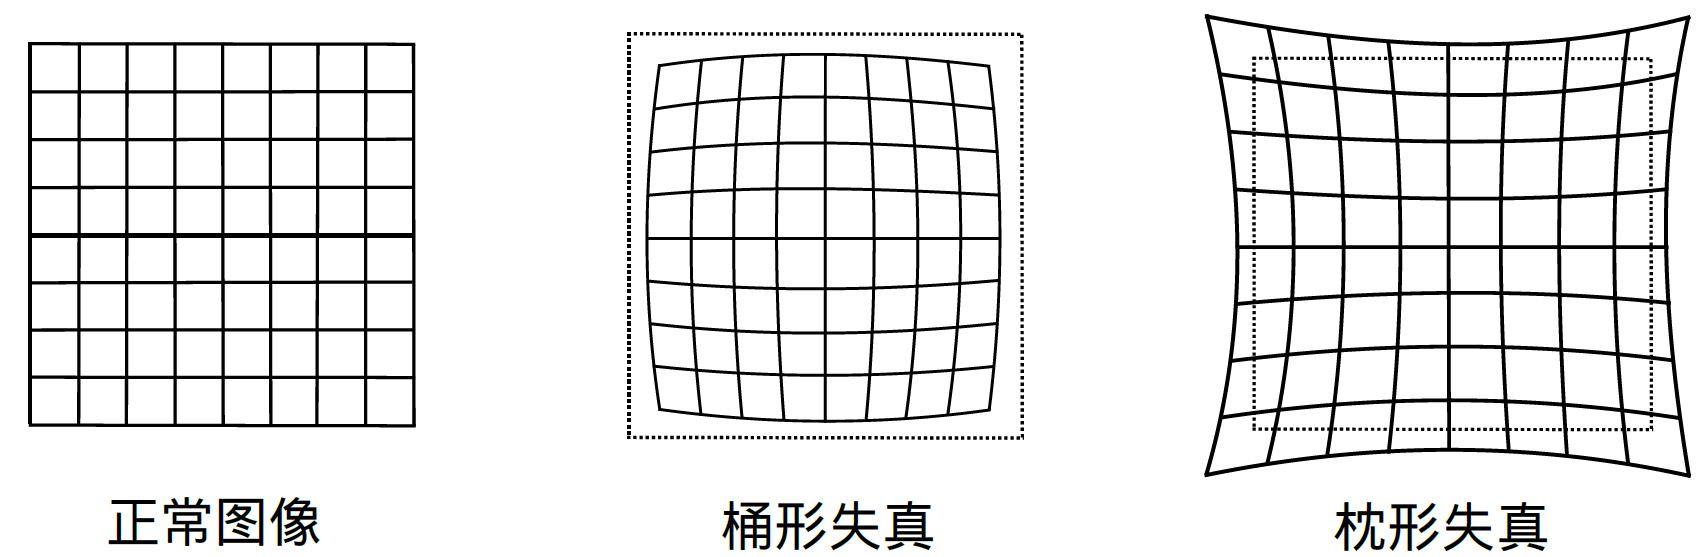
\includegraphics[width=0.7\textwidth]{figures/chapter2/fig2_2}
	\caption{两种类型的径向畸变}\label{fig2_2}
\end{figure}

切向畸变示意图如图\ref{fig2_3}。设归一化成像平面上的点$p $的笛卡尔坐标为 $[x, y]^{T} $ ,极坐标为 $[r, \theta]^{T} $ 。径向畸变使坐标点的长度 $r $ 变化了$\delta r $  ,切向畸变使坐标点的水平夹角 $\theta$ 变化了$\delta \theta $  。
\begin{figure}[h]\setlength{\belowcaptionskip}{-12pt}
	\centering
	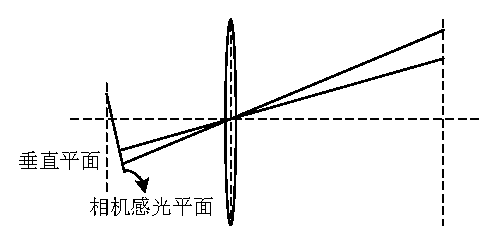
\includegraphics[width=0.5\textwidth]{figures/chapter2/fig2_3}
	\caption{切向畸变示意图}\label{fig2_3}
\end{figure}

使用一个函数来表达径向畸变前后坐标的变化:
\begin{equation}
\label{eqn:2.12}
\left\{\begin{aligned} x_{\text {corrected}} &=x\left(1+k_{1} r^{2}+k_{2} r^{4}+k_{3} r^{6}\right) \\ y_{\text {corrected}} &=y\left(1+k_{1} r^{2}+k_{2} r^{4}+k_{3} r^{6}\right) \end{aligned}\right.
\end{equation}
其中,$\left[x_{\text {corrected }}, y_{\text {corrected}}\right]^{T} $ 表示去畸变后的坐标。公式(\ref{eqn:2.12})中,越靠近图像中心,畸变越小,畸变系数 $k_1$  起主导作用。越远离图像中心,畸变越大,畸变系数 $k_2$ 起主导作用。一般的针孔相机用这两个系数就能去除径向畸变。对于像鱼眼镜头等畸变较大的相机,可以加入 $k_3$  来去畸变。

对于切向畸变,可以使用参数$p_1,p_2$来进行去畸变:
\begin{equation}
\label{eqn:2.13}
\left\{
\begin{aligned} 
x_{\text {corrected}} &=x+2 p_{1} x y+p_{2}\left(r^{2}+2 x^{2}\right) \\ 
y_{\text {corrected}} &=y+p_{1}\left(r^{2}+2 y^{2}\right)+2 p_{2} x y 
\end{aligned}
\right.
\end{equation}

由式(\ref{eqn:2.12})和式(\ref{eqn:2.13})可以得到坐标点在归一化成像平面上去除径向畸变和切向畸变后的正确坐标点:
\begin{equation}
\label{eqn:2.14}
\left\{
\begin{aligned}
x_{\text {corrected}}&=x\left(1+k_{1} r^{2}+k_{2} r^{4}+k_{3} r^{6}\right)+2 p_{1} x y+p_{2}\left(r^{2}+2 x^{2}\right) \\ 
y_{\text {corrected}}&=y\left(1+k_{1} r^{2}+k_{2} r^{4}+k_{3} r^{6}\right)+p_{1}\left(r^{2}+2 y^{2}\right)+2 p_{2} x y
\end{aligned}
\right.
\end{equation}
进一步,通过内参矩阵可以得到去畸变后的像素坐标:
\begin{equation}
\label{eqn:2.15}
\left\{
\begin{aligned}
u_{\text {corrected}}&=f_{x} x_{\text {corrected}}+c_{x} \\ 
v_{\text {corrected}}&=f_{y} y_{\text {corrected}}+c_{y}
\end{aligned}
\right.
\end{equation}
\subsection{IMU状态模型}
四元数可表示为:
\begin{equation}
\setlength{\abovedisplayskip}{6pt}
\setlength{\belowdisplayskip}{6pt}
\label{eqn:2.16}
\mathbf{q}=q_{w}+q_{x} i+q_{y} j+q_{z} k \quad \Leftrightarrow \quad \mathbf{q}=q_{w}+\mathbf{q}_{v}
\end{equation}
其中,$i,j,k$ 是四元数的虚部,满足:
\begin{equation}
\label{eqn:2.17}
\left\{\begin{array}{l}{i^{2}=j^{2}=k^{2}=-1} \\ {i j=k, j i=-k} \\ {j k=i, k j=-i} \\ {k i=j, i k=-j}\end{array}\right.
\end{equation}
也可以用一个四维向量来表示:
\begin{equation}
\label{eqn:2.18}
\mathbf{q} \triangleq \left[ \begin{array}{cc}
{q_{w}} & {\mathbf{q}_{v} }
\end{array}\right] = \left[ \begin{array}{cccc}
{q_{w}} & {q_{x}} & {q_{y}} & {q_{z} } \end{array}\right]^{T}
\end{equation}
设有两个四元数 $\mathbf{p}, \mathbf{q} $ ,那么四元数的运算可表示如下:\\
(1)加法和减法:
\begin{equation}
\label{eqn:2.19}
\mathbf{p} \pm \mathbf{q}=\left[ \begin{array}{c}{p_{w}} \\ {\mathbf{p}_{v}}\end{array}\right] \pm \left[ \begin{array}{c}{q_{w}} \\ {\mathbf{q}_{v}}\end{array}\right]=\left[ \begin{array}{c}{p_{w} \pm q_{w}} \\ {\mathbf{p}_{v} \pm \mathbf{q}_{v}}\end{array}\right]
\end{equation}
满足交换律和结合律,
\begin{equation}
\label{eqn:2.20}
\mathbf{p}+\mathbf{q}=\mathbf{q}+\mathbf{p}
\end{equation}
\begin{equation}
\label{eqn:2.21}
\mathbf{p}+(\mathbf{q}+\mathbf{r})=(\mathbf{p}+\mathbf{q})+\mathbf{r}
\end{equation}
(2)乘法:
\begin{equation}
\label{eqn:2.22}
\mathbf{p} \otimes \mathbf{q}=\left[ \begin{array}{c}{p_{w} q_{w}-p_{x} q_{x}-p_{y} q_{y}-p_{z} q_{z}} \\ {p_{w} q_{x}+p_{x} q_{w}+p_{y} q_{z}-p_{z} q_{y}} \\ {p_{w} q_{y}-p_{x} q_{z}+p_{y} q_{w}+p_{z} q_{x}} \\ {p_{w} q_{z}+p_{x} q_{y}-p_{y} q_{x}+p_{z} q_{w}}\end{array}\right]
\end{equation}
其中, $\otimes$ 表示四元数相乘。写成标量和矢量部分,
\begin{equation}
\label{eqn:2.23}
\mathbf{p} \otimes \mathbf{q}=\left[ \begin{array}{c}{p_{w} q_{w}-\mathbf{p}_{v}^{\top} \mathbf{q}_{v}} \\ {p_{w} \mathbf{q}_{v}+q_{w} \mathbf{p}_{v}+\mathbf{p}_{v} \times \mathbf{q}_{v}}\end{array}\right]
\end{equation}
不满足交换律,
\begin{equation}
\label{eqn:2.24}
\mathbf{p} \otimes \mathbf{q} \neq \mathbf{q} \otimes \mathbf{p}
\end{equation}
满足结合律和分配律,
\begin{equation}
\label{eqn:2.25}
(\mathbf{p} \otimes \mathbf{q}) \otimes \mathbf{r}=\mathbf{p} \otimes(\mathbf{q} \otimes \mathbf{r})
\end{equation}
\begin{equation}
\label{eqn:2.26}
\mathbf{p} \otimes(\mathbf{q}+\mathbf{r})=\mathbf{p} \otimes \mathbf{q}+\mathbf{p} \otimes \mathbf{r} \quad  
\text{and}
\quad(\mathbf{p}+\mathbf{q}) \otimes \mathbf{r}=\mathbf{p} \otimes \mathbf{r}+\mathbf{q} \otimes \mathbf{r}
\end{equation}
两个四元数的乘积可以等效的表示为两个矩阵的乘积,
\begin{equation}
\label{eqn:2.27}
\setlength{\abovedisplayskip}{6pt}
\setlength{\belowdisplayskip}{6pt}
\mathbf{q}_{1} \otimes \mathbf{q}_{2}=\left[\mathbf{q}_{1}\right]_{L} \mathbf{q}_{2} \quad \text { and } \quad \mathbf{q}_{1} \otimes \mathbf{q}_{2}=\left[\mathbf{q}_{2}\right]_{R} \mathbf{q}_{1}
\end{equation}
其中 $\left[\mathbf{q}\right]_{L}$ 和 $\left[\mathbf{q}\right]_{R}$ 分别为,
\begin{equation}
\label{eqn:2.28}
[\mathbf{q}]_{L}=\left[ \begin{array}{cccc}{q_{w}} & {-q_{x}} & {-q_{y}} & {-q_{z}} \\ {q_{x}} & {q_{w}} & {-q_{z}} & {q_{y}} \\ {q_{y}} & {q_{z}} & {q_{w}} & {-q_{x}} \\ {q_{z}} & {-q_{y}} & {q_{x}} & {q_{w}}\end{array}\right], \quad[\mathbf{q}]_{R}=\left[ \begin{array}{cccc}{q_{w}} & {-q_{x}} & {-q_{y}} & {-q_{z}} \\ {q_{x}} & {q_{w}} & {q_{z}} & {-q_{y}} \\ {q_{y}} & {-q_{z}} & {q_{w}} & {q_{x}} \\ {q_{z}} & {q_{y}} & {-q_{x}} & {q_{w}}\end{array}\right]
\end{equation}
或者,
\begin{equation}
\label{eqn:2.29}
[\mathbf{q}]_{L}=q_{w} \mathbf{I}+\left[ \begin{array}{cc}{0} & {-\mathbf{q}_{v}^{\top}} \\ {\mathbf{q}_{v}} & {\left[\mathbf{q}_{v}\right]_{ \times}}\end{array}\right], \quad[\mathbf{q}]_{R}=q_{w} \mathbf{I}+\left[ \begin{array}{cc}{0} & {-\mathbf{q}_{v}^{\top}} \\ {\mathbf{q}_{v}} & {-\left[\mathbf{q}_{v}\right]_{ \times}}\end{array}\right]
\end{equation}
这里,用运算符 $[\bullet]_{\times} $ 产生反对称矩阵,
\begin{equation}
\label{eqn:2.30}
[\mathbf{a}]_{ \times} \triangleq \left[ \begin{array}{ccc}{0} & {-a_{z}} & {a_{y}} \\ {a_{z}} & {0} & {-a_{x}} \\ {-a_{y}} & {a_{x}} & {0}\end{array}\right]
\end{equation}
因为,
\begin{equation}
\label{eqn:2.31}
(\mathbf{q} \otimes \mathbf{x}) \otimes \mathbf{p}=[\mathbf{p}]_{R}[\mathbf{q}]_{L} \mathbf{x} \quad \text { and } \quad \mathbf{q} \otimes(\mathbf{x} \otimes \mathbf{p})=[\mathbf{q}]_{L}[\mathbf{p}]_{R} \mathbf{x}
\end{equation}
所以,
\begin{equation}
\label{eqn:2.32}
[\mathbf{p}]_{R}[\mathbf{q}]_{L}=[\mathbf{q}]_{L}[\mathbf{p}]_{R}
\end{equation}
(3)共轭:
\begin{equation}
\label{eqn:2.33}
\mathbf{q}^{*} \triangleq q_{w}-\mathbf{q}_{v}=\left[ \begin{array}{cc}{q_{w}} & {-\mathbf{q}_{v}}\end{array}\right]^T
\end{equation}
有以下特性,
\begin{equation}
\label{eqn:2.34}
\mathbf{q} \otimes \mathbf{q}^{*}=\mathbf{q}^{*} \otimes \mathbf{q}=q_{w}^{2}+q_{x}^{2}+q_{y}^{2}+q_{z}^{2}=\left[ \begin{array}{c}{q_{w}^{2}+q_{x}^{2}+q_{y}^{2}+q_{z}^{2}} \\ {\mathbf{0}_{v}}\end{array}\right]
\end{equation}
\begin{equation}
\label{eqn:2.35}
(\mathbf{p} \otimes \mathbf{q})^{*}=\mathbf{q}^{*} \otimes \mathbf{p}^{*}
\end{equation}
(4)范数:
\begin{equation}
\label{eqn:2.36}
\|\mathbf{q}\| \triangleq \sqrt{\mathbf{q} \otimes \mathbf{q}^{*}}=\sqrt{\mathbf{q}^{*} \otimes \mathbf{q}}=\sqrt{q_{w}^{2}+q_{x}^{2}+q_{y}^{2}+q_{z}^{2}} \in \mathbb{R}
\end{equation}
(5)逆:
\begin{equation}
\label{eqn:2.37}
\mathbf{q}^{-1}=\mathbf{q}^{*} /\|\mathbf{q}\|^{2}
\end{equation}
\begin{equation}
\label{eqn:2.38}
\mathbf{q} \otimes \mathbf{q}^{-1}=\mathbf{q}^{-1} \otimes \mathbf{q}=\mathbf{q}_{1}
\end{equation}
(6)单位四元数:

对于单位四元数,因为$\|\mathbf{q}\|=1 $ ,所以,
\begin{equation}
\label{eqn:2.39}
\setlength{\abovedisplayskip}{6pt}
\setlength{\belowdisplayskip}{6pt}
\mathbf{q}^{-1}=\mathbf{q}^{*}
\end{equation}
当把单位四元数解释为方向变换或旋转算子时,这个性质意味着可以用共轭四元数实现相反的旋转。单位四元数总是可以写成这种形式,
\begin{equation}
\label{eqn:2.40}
\setlength{\abovedisplayskip}{6pt}
\setlength{\belowdisplayskip}{6pt}
\mathbf{q}=\left[ \begin{array}{cc}{\cos \theta} & {\mathbf{u} \sin \theta}\end{array}\right]^T
\end{equation}
其中,$\mathbf{u}=u_{x} i+u_{y} j+u_{z} k $ 为单位向量, $\theta $为标量。
IMU状态模型主要由运动模型以及观测和噪声模型构成\upcite{sola2017quaternion},状态量包括:$[\mathbf{p}_t, \mathbf{v}_t, \mathbf{q}_t, \mathbf{b}_{a_t}, \bm{b}_{\omega_t},\mathbf{g}^w]$
 ,分别表示 $t$  时刻IMU的位置,速度,姿态(旋转),加速度bias,角速度bias以及世界坐标系下的重力向量。根据式(\ref{eqn:2.22})(\ref{eqn:2.27})(\ref{eqn:2.28})(\ref{eqn:2.29})(\ref{eqn:2.40})可得,
\begin{equation}
\label{eqn:2.41}
\begin{aligned} 
\dot{\mathbf{q}}_{t} &= \lim _{\delta t \rightarrow 0} \frac{1}{\delta t}\left(\mathbf{q}_{t+\delta t}-\mathbf{q}_{t}\right) \\
&= \lim _{\delta t \rightarrow 0} \frac{1}{\delta t}\left(\mathbf{q}_{t} \otimes \delta {\mathbf{q}_{t}}-\mathbf{q}_{t} \otimes \left[ \begin{array}{l}{0} \\ {1}\end{array}\right]\right) \\
&= \lim _{\delta t \rightarrow 0} \frac{1}{\delta t}\left(\mathbf{q}_{t} \otimes \left[ \begin{array}{c}{\mathbf{u} \sin \frac{\theta}{2}} \\ {\cos \frac{\theta}{2}}\end{array}\right]-\mathbf{q}_{t} \otimes \left[ \begin{array}{l}{0} \\ {1}\end{array}\right]\right) \\
& \approx \lim _{\delta t \rightarrow 0} \frac{1}{\delta t} \left( \mathbf{q}_{t} \otimes \left[ \begin{array}{c}{\mathbf{u} \frac{\theta}{2}} \\ {1}\end{array}\right]-\mathbf{q}_{t} \otimes \left[ \begin{array}{l}{0} \\ {1}\end{array}\right] \right) \\
&= \lim _{\delta t \rightarrow 0} \frac{1}{\delta t} \left( \left[ \left[ \begin{array}{c}{\mathbf{u} \frac{\theta}{2}} \\ {1}\end{array}\right]\right]_R-\left[\left[ \begin{array}{l}{0} \\ {1}\end{array}\right]\right]_R \right) \mathbf{\mathbf{q}}_t \\
&= \lim _{\delta t \rightarrow 0} \frac{1}{\delta t} \left[ \begin{array}{cc}{-\frac {[\theta]_{\times}} {2}} & {\frac{\theta}{2}} \\ {-\frac{\theta^{T}}{2}} & {0}\end{array}\right]\mathbf{\mathbf{q}}_t
\end{aligned} 
\end{equation}
其中 $\delta \mathbf{q}_t $ 表示在 $t$  时刻加的三维小扰动。又因为角速度为:
\[
\setlength{\abovedisplayskip}{6pt}
\setlength{\belowdisplayskip}{6pt}
{\omega}=\lim _{\delta t \rightarrow 0} \frac{\theta}{\delta t} 
\]
所以式(\ref{eqn:2.41})可以化简为:
\begin{equation}
\label{eqn:2.42}
\begin{aligned}
\dot{\mathbf{q}}_{t}&=\frac{1}{2} \left[ \begin{array}{cc}{-[\omega]_{\times}} & {\omega} \\ {-\omega^{T}} & {0}\end{array}\right] \mathbf{q}_{t} \\  
&= \frac{1}{2} \bm{\Omega}(\omega) \mathbf{q}_{t} \\
&= \frac{1}{2} {\left[\left[ \begin{array}{l}{\omega} \\ {0}\end{array}\right]\right]}_R \mathbf{q}_{t} \\
&= \frac{1}{2} \left[\mathbf{q}_{t}\right]_L \otimes \left[ \begin{array}{l}{\omega} \\ {0}\end{array}\right]
\end{aligned}
\end{equation}
假设,$\mathbf{a}_t $ 和$\bm{\omega}_t $ 表示IMU真实的加速度和角速率。假设用$\hat{\textbf{a}}_t $ 和 $\hat{\bm{\omega}}_t $表示加速度和角速率的观测值,即传感器读数,测量噪声为$\mathbf{n}_a $ 和$\mathbf{n}_w $ ,那么,
\begin{equation}
\label{eqn:2.43}
\setlength{\abovedisplayskip}{6pt}
\setlength{\belowdisplayskip}{6pt}
\begin{split}
\hat{\textbf{a}}_t&=\textbf{a}_t+{\textbf{b}_a}_t+\textbf{R}_w^t\textbf{g}^w+\textbf{n}_a \\
\hat{\bm{\omega}}_t&=\bm{\omega}_t+\mathbf{b}_{w_t}+\mathbf{n}_w.
\end{split}
\end{equation}
其中$\mathbf{R}_w^t $ 的作用是将重力矢量从世界坐标系下变换到IMU坐标系下。需要注意的是,式(\ref{eqn:2.43})忽略了地球自转角速率$\bm{\omega}_\mathcal{E} $ ,否则将是:$\hat{\bm{\omega}}_t=\bm{\omega}_t+ \mathbf{R}_w^t \bm{\omega}_\mathcal{E} +\mathbf{b}_{w_t}+\mathbf{n}_w $ 。在大多数情况下,不需要考虑地球自转,但是,当使用的IMU传感器分辨率很高,且具有非常小的噪声和bias时, $\bm{\omega}_\mathcal{E} $可能会被传感器测量到( $\bm{\omega}_\mathcal{E} = {15}^{\circ}/h \approx 7.3×10^{-5} rad/s $)。在这种情况下,为了保持IMU误差模型的有效性,在公式中不应该忽略$\bm{\omega}_\mathcal{E} $ 。

由式(\ref{eqn:2.43})可以得到IMU真实的加速度$\mathbf{a}_t $和角速率 $\bm{\omega}_t $:
\begin{equation}
\label{eqn:2.44}
\setlength{\abovedisplayskip}{6pt}
\setlength{\belowdisplayskip}{6pt}
\begin{split}
\textbf{a}_t &=  \hat{\textbf{a}}_t - {\textbf{b}_a}_t - \textbf{R}_w^t\textbf{g}^w - \textbf{n}_a \\
\bm{\omega}_t   &=  \hat{\bm{\omega}}_t  - \mathbf{b}_{w_t} - \mathbf{n}_w.
\end{split}
\end{equation}
IMU的测量值是在IMU自身坐标系下测量得到的,其中包含了重力矢量,并且受到加速度bias、陀螺仪bias以及附加测量噪声的影响。假设加速度计和陀螺仪附加的测量噪声为高斯白噪声,$\mathbf{n}_a\sim\mathcal{N}(0,\bm{\sigma}_a^2) $ ,$\mathbf{n}_w\sim\mathcal{N}(0,\bm{\sigma}_w^2) $ 。加速度计bias和陀螺仪bias被建模为随机游走,随机游走是一个离散模型。将维纳过程(Wiener Process)\upcite{orey1973sample}离散化就是随机游走。而Wiener Process是高斯白噪声的积分,故其导数为高斯分布模型,$\mathbf{n}_{b_a}\sim\mathcal{N}(0,\bm{\sigma}_{b_a}^2) $ ,$\mathbf{n}_{b_w}\sim\mathcal{N}(0,\bm{\sigma}_{b_w}^2) $ 。所以,可得:
\begin{equation}
\label{eqn:2.45}
\setlength{\abovedisplayskip}{6pt}
\setlength{\belowdisplayskip}{6pt}
\dot{\mathbf{b}}_{a_t}=\mathbf{n}_{b_a},\qquad \dot{\mathbf{b}}_{w_t}=\mathbf{n}_{b_w}
\end{equation}
所以,IMU的运动方程为:
\begin{equation}
\label{eqn:2.46}
\left\{
\begin{aligned} \dot{\mathbf{p}}_{t} &=\mathbf{v}_{t} \\ 
\dot{\mathbf{v}}_{t} &=\mathbf{a}_{t} = \hat{\textbf{a}}_t - {\textbf{b}_a}_t - \textbf{R}_w^t\textbf{g}^w - \textbf{n}_a \\ 
\dot{\mathbf{q}}_{t} &=  \frac{1}{2} \bm{\Omega}(\omega) \mathbf{q}_{t} = \frac{1}{2} \bm{\Omega}\left(\hat{\bm{\omega}}_t  - \mathbf{b}_{w_t} - \mathbf{n}_w \right) \mathbf{q}_{t} \\ 
\dot{\mathbf{b}}_{a_t} &=\mathbf{n}_{b_a} \\ 
\dot{\mathbf{b}}_{w_t} &=\mathbf{n}_{b_w} \\ 
\dot{\mathbf{g}}^{w} &=0 \end{aligned}
\right.
\end{equation}
\subsection{磁力计数学模型}
磁力计也叫电子罗盘,能够测量地球磁场分布,进而计算载体的航向信息\upcite{butala2017modeling}。如图\ref{fig2_4}所示,是地球磁场分布图。地球是一个硕大的磁体,磁感线方向从南极到北极。在磁场的南北两极,磁场垂直于水平面,靠近地球赤道,磁场方向平行于水平面。值得注意的是地球磁场的两极和地球地理两极并不完全的重合,他们之间大约有11°的夹角。

地球上某一点的磁场可以用一个矢量 $\mathbf{H} $来表示,矢量$\mathbf{H} $ 的大小和方向分别代表该点磁场的强度和磁场的方向。如图\ref{fig2_5}所示,矢量$\mathbf{H} $ 可以被分解为两个水平分量 $\mathbf{H}_x,\mathbf{H}_y$ ,和一个垂直分量 $\mathbf{H}_z$ 。 $\alpha$是要求的航向角,它是载体当前的正前方与磁北的夹角。航向角的变化值域是0°$\sim $ 360°。
\begin{figure}[h]\setlength{\belowcaptionskip}{-12pt}
	\centering	
	\begin{minipage}[t]{0.35\linewidth}				
		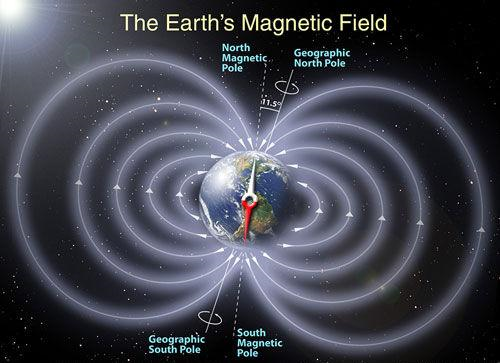
\includegraphics[height=4cm,width=5cm]{figures/chapter2/fig2_4}		
		\caption{地球磁场分布图}	\label{fig2_4}	
	\end{minipage}%	
	\hspace{0.1in}	
	\begin{minipage}[t]{0.5\linewidth}		
		\centering		
		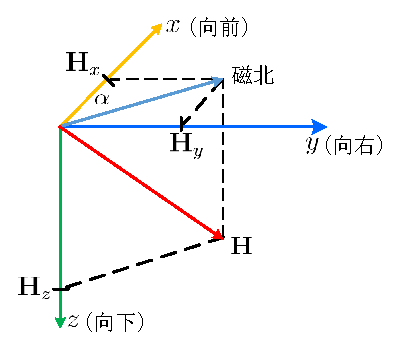
\includegraphics[height=5cm,width=6.5cm]{figures/chapter2/fig2_5}		
		\caption{地磁场矢量分解示意图} \label{fig2_5}		
	\end{minipage}	
\end{figure}
当磁力计水平放置时,磁场矢量$\mathbf{H} $ 在重力方向 $z$ 轴上的分量$\mathbf{H}_z $ 为零,此时$\alpha$ 为:
\begin{equation}
\label{eqn:2.47}
\alpha = \text{arctan}\left(\frac{\mathbf{H}_y}{\mathbf{H}_x}\right)
\end{equation}
但是,通常情况下磁力计不会和水平面完全平行,他们之间会有一个夹角,这个时候就不能通过式(\ref{eqn:2.47})来计算$\alpha$ 的值。需要用加速度计来补偿这个夹角。假设磁力计和加速度计的坐标系重合,在静止或者匀速直线运动的情况下,加速度计测量的三个轴向的加速度是重力加速度在三个轴向的分量。假设在$x,y,z $ 三个轴的测得的重力分量分别为$\mathbf{g}_x, \mathbf{g}_y,\mathbf{g}_z$ ,那么横滚角 $\gamma $和俯仰角$\theta$ 分别为:
\begin{equation}
\label{eqn:2.48}
\begin{aligned}
\gamma &= \text{arctan}\left(\frac{\mathbf{g}_y}{\mathbf{g}_z}\right) \\
\theta &= \text{arcsin}\left( \frac{-\mathbf{g}_x}{\mathbf{g}}\right)
\end{aligned}
\end{equation}
假设磁力计输出的三轴磁分量为$\mathbf{M}_x,\mathbf{M}_y,\mathbf{M}_z $ ,可以根据载体的横滚角 和俯仰角 计算出当地磁场的水平分量$\mathbf{H}_x, \mathbf{H}_y $ :
\begin{equation}
\label{eqn:2.49}
\setlength{\abovedisplayskip}{6pt}
\setlength{\belowdisplayskip}{6pt}
\begin{aligned}
\mathbf{H}_x &= \mathbf{M}_x \text{cos}\theta + \mathbf{M}_y\text{sin}\theta\text{sin}\gamma + \mathbf{M}_z \text{sin}\theta\text{cos}\gamma \\
\mathbf{H}_y &= \mathbf{M}_z\text{sin}\gamma  - \mathbf{M}_y \text{cos}\gamma
\end{aligned}
\end{equation}
将式(\ref{eqn:2.49})代入式(\ref{eqn:2.48})可得航向角 :
\begin{equation}
\label{eqn:2.50}
\alpha = \text{arctan}\left(
\frac{\mathbf{M}_z\text{sin}\gamma  - \mathbf{M}_y \text{cos}\gamma}
{\mathbf{M}_x \text{cos}\theta + \mathbf{M}_y\text{sin}\theta\text{sin}\gamma + \mathbf{M}_z \text{sin}\theta\text{cos}\gamma }\right)
\end{equation}
\subsection{传感器选型}
考虑到本系统的应用环境以及相机和IMU之间需要硬件同步等需求,所以需要慎重选择满足需求的相机和IMU。

(1)单目相机及镜头选型

首先,考虑使用全局快门相机还是卷帘快门相机,这两种相机的成像方式有区别。如图\ref{fig2_6},全局相机是一次性成像,所有像素同时开始和停止曝光,而卷帘相机是逐行成像,每个像素曝光时间不同。因此当拍摄物体运动速度越快,卷帘相机的“果冻效应”就越明显,如图\ref{fig2_7}左图所示。图\ref{fig2_7}右图是的全局快门相机拍摄的图片,可以看到虽然出现了图像模糊问题,但是并没有出现“果冻效应”。对于SLAM系统,高速运动是普遍存在的,因此为了提高系统的鲁棒性,本文选用全局快门相机。其次,对于视觉SLAM系统来说,不需要彩色的图像,利用黑白的图像就可以进行特征点提取与匹配,所以选取灰色相机即可。而且,相机的视角不能太小,太小的话容易导致特征跟踪失败。考虑到室外的环境,相机焦距也不能太短,否则远处的场景会模糊。最后,为了让相机能够在不同的季节和地区正常工作,应该选取具有宽温特性的工业相机。
\begin{figure}[h]\setlength{\belowcaptionskip}{-2pt}
	\centering
	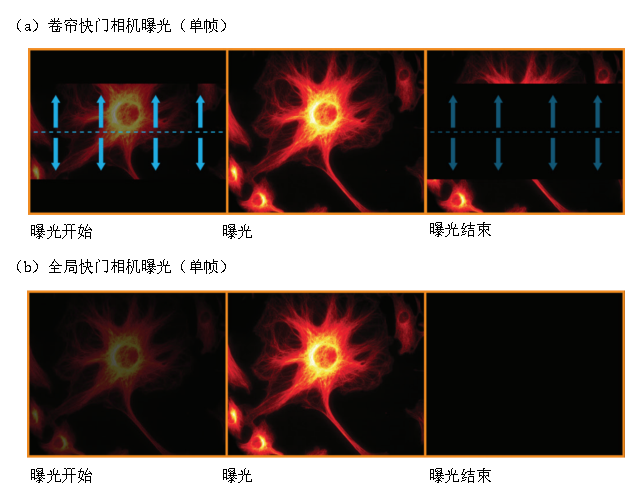
\includegraphics[width=0.7\textwidth]{figures/chapter2/fig2_6}
	\caption{全局相机和卷帘快门相机成像方式}\label{fig2_6}
\end{figure}
\begin{figure}[h]\setlength{\belowcaptionskip}{-12pt}
	\centering
	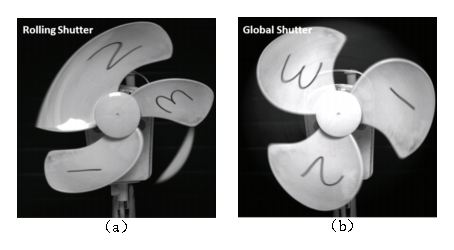
\includegraphics[width=0.5\textwidth]{figures/chapter2/fig2_7}
	\caption{高速运动下的(a)卷帘快门相机图像;(b)全局相机图像}\label{fig2_7}
\end{figure}

基于以上分析,本系统选择灰点公司的Grasshopper3-USB3单目相机,如图\ref{fig2_8}所示。采用快速、高灵敏度的CMOS芯片——IMX174,可提供最高1920×1200的图像分辨率,最高帧率达到163FPS。该相机采用USB 3.0接口,非常适合于处理由传感器产生的远远超过360MByte/s的高速数据传输率,并且比其他高速数字接口更具成本效益。该相机的参数如表\ref{tab2.1}所示。
\begin{figure}[h]\setlength{\belowcaptionskip}{8pt}
	\centering
	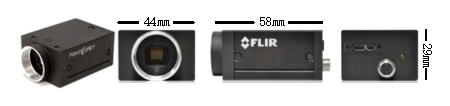
\includegraphics[width=0.7\textwidth]{figures/chapter2/fig2_8}
	\caption{Grasshopper3-USB3相机及其三视图}\label{fig2_8}
\end{figure}
\begin{table}\setlength{\belowcaptionskip}{-12pt}
	\zihao{5}  
	\centering
	\caption{相机参数} \label{tab2.1}
	\begin{tabular}{m{0.15\textwidth}<{\centering} m{0.4\textwidth}<{\centering}}%
		\toprule
		型 \quad\quad 号			&GS3-U3-123S6M-C	 \\
		 \midrule
		分 \ \  辨 \ \  率	       &1920 x 1200         \\
		 \midrule
		帧 \quad\quad 率	    	&163 FPS	         \\
		 \midrule
		传 \ \  感 \ \  器	   &Sony IMX174, CMOS, 1/1.2"	 \\
		 \midrule
		快门方式	              &全局快门             \\
		\midrule
		模数转换                  &10位/12位           \\
		\midrule
		曝光时间                  &0.005 ms ~ 31.9 s   \\
		\midrule
		触发方式                  &Standard, bulb, overlapped, multi-shot \\
		\midrule
		输出格式                  &Mono8, Mono12, Mono16\\
		\midrule
		数据接口                  &USB 3.0                \\
		\midrule
		传输速率                  &5 Gbit/s                \\
		\midrule
		存 \quad\quad 储          &128MB帧缓存,2MB永久闪存    \\
		\midrule
		外观尺寸                  &44 mm×29 mm×58 mm        \\
		\midrule
		重 \quad\quad 量          &90g                    \\
		\midrule
		功 \quad\quad 耗          &≤4.5 W                 \\
		\midrule
		镜头接口                  &C                      \\
		\midrule
		工作温度 	              &0℃~ +50℃               \\
		\bottomrule
	\end{tabular}
\end{table}

相机镜头选用沃乐斯WL1412-1K-1工业定焦镜头,其外观和尺寸如图\ref{fig2_9}所示。表\ref{tab2.2}是沃乐斯WL1412-1K-1镜头参数。
\begin{figure}[!h]\setlength{\belowcaptionskip}{8pt}
	\centering
	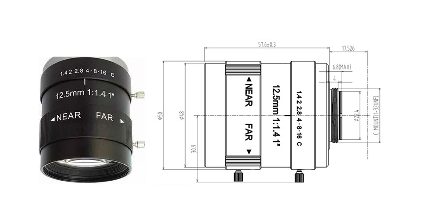
\includegraphics[width=0.45\textwidth]{figures/chapter2/fig2_9}
	\caption{沃乐斯WL1412-1K-1镜头}\label{fig2_9}
\end{figure}
\begin{table}[!h]\setlength{\belowcaptionskip}{-12pt}
	\zihao{5}  
	\centering
	\caption{沃乐斯WL1412-1K-1镜头参数} \label{tab2.2}
	\begin{tabular}{m{0.13\textwidth}<{\centering} m{0.4\textwidth}<{\centering}}%
		\toprule
		型 \quad\quad 号			&GS3-U3-123S6M-C	 \\
		\midrule
		焦 \quad\quad 距	       &1920 x 1200         \\
		\midrule
		接 \quad\quad 口	    	&163 FPS	         \\
		\midrule
		光圈范围	   &Sony IMX174, CMOS, 1/1.2"	 \\
		\midrule
		视 \ \  场\ \  角	              &全局快门             \\
		\midrule
		后 \ \  焦 \ \  距                  &10位/12位           \\
		\midrule
		畸 \ \  变 \ \  率                  &0.005 ms ~ 31.9 s   \\
		\midrule
		分 \ \  辨 \ \  率                  &Standard, bulb, overlapped, multi-shot \\
		\midrule
		外观尺寸                  &Mono8, Mono12, Mono16\\
		\midrule
		工作温度                  &USB 3.0                \\
		\midrule
		重 \quad\quad 量                  &5 Gbit/s                \\
		\bottomrule
	\end{tabular}
\end{table}

(2)IMU选型。

考虑到本系统主要在汽车或无人机上使用,所以光纤陀螺和激光陀螺等大型的高精度惯性器件虽然精度很高,但是通常体积大、重量大,所以不适用于本系统。而MEMS体积小,重量轻,非常适合车载和机载。但是普通的低价MEMS往往精度低,噪声大,会严重影响系统的输出精度。所以,需要尽可能的在成本可接受范围内选择一款相对来说精度高,噪声小,而且具备宽温特性的MEMS。

通过以上分析以及多方对比,本系统的IMU选用挪威Sensonor公司的STIM300。STIM300提供了一个可供外部同步信号输入的IO口和一个与自身采样频率相同的同步方波输出IO口。STIM300及其尺寸图如图\ref{fig2_10}。表\ref{tab2.3}是STIM300的性能参数。
\begin{figure}[!h]\setlength{\belowcaptionskip}{-12pt}
	\centering
	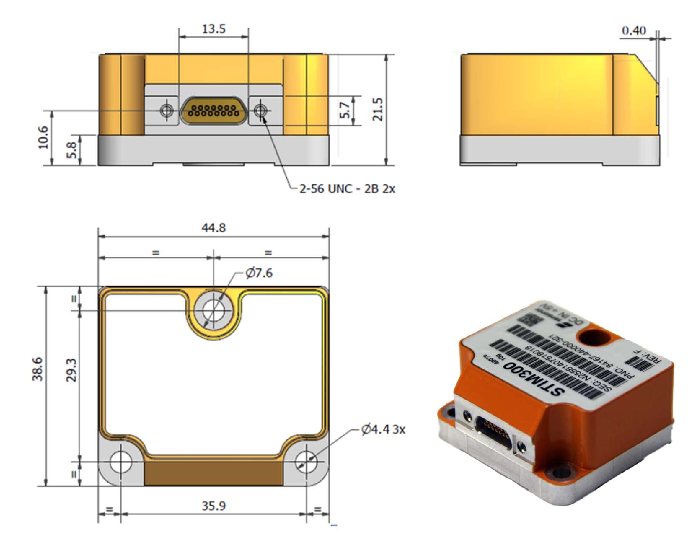
\includegraphics[width=0.6\textwidth]{figures/chapter2/fig2_10}
	\caption{STIM300及其尺寸}\label{fig2_10}
\end{figure}
\begin{table}[!h]
	\zihao{5}  
	\centering
	\caption{STIM300性能参数} \label{tab2.3}
	\begin{tabular}{m{0.13\textwidth}<{\centering} m{0.13\textwidth}<{\centering} m{0.13\textwidth}<{\centering} m{0.13\textwidth}<{\centering} m{0.13\textwidth}<{\centering} m{0.13\textwidth}<{\centering}}%
		\toprule
		\multicolumn{2}{c}{整体指标}  &\multicolumn{2}{c}{陀螺仪性能}       & \multicolumn{2}{c}{加速度计性能}  \\
		\midrule
		重 \quad\quad 量  &	55g	    &测量范围  &	±400°/s	             &测量范围  & ±10g \\
		\midrule
		输出形式          &	RS422     &零\quad\quad 偏  & 0.3°/h           &零\quad\quad 偏  &	0.05mg \\
		\midrule
		工作温度	      & -20℃~ +85℃     &随机游走 & 0.15°/$\sqrt{h}$ 
  &随机游走 & 0.07m/s°/$\sqrt{h}$ \\ 	
		\midrule
		工作电压	      & 5V±0.5V	      &分 \ \  辨 \ \  率   & 0.22°/h	&分 \ \  辨 \ \  率 &	1.9ug \\
		\midrule
		功\quad\quad 耗  & <1.5W	    &全温零偏	   &  ±10°/h rms	   &全温零偏  & ±2mg rms \\
		\midrule
		采样频率  & ≤2kHz & & & & \\
		\bottomrule
	\end{tabular}
\end{table}

值得注意的是,由于本文中视觉/惯性融合系统是紧耦合系统,需要尽可能准确的时间同步,所以需要相机和IMU在硬件上进行同步。这就要求传感器具有触发或者被触发的功能,可以是相机触发IMU,也可以是IMU触发相机。
\section{传感器的标定与同步}
尽管传感器在出厂时已经确定了具体的参数和指标,但是鉴于出厂时不可避免的有安装误差,以及传感器精度会随着使用环境的变化而变化,在使用传感器时有必要对其进行标定。
\subsection{相机标定}
\label{chap:2.2.1}
表\ref{tab2.4} 总结了常见的相机标定方法及其优缺点。
\begin{table}[h]\setlength{\abovecaptionskip}{6pt}
	\zihao{5}  
	\newcommand{\tabincell}[2]{\begin{tabular}{@{}#1@{}}#2\end{tabular}}  %导言区
	\centering
	\caption{常见的相机标定方法及其优缺点} \label{tab2.4}
	\begin{tabular}{m{0.1\textwidth}<{\centering} m{0.2\textwidth}<{\centering} m{0.2\textwidth}<{\centering} m{0.1\textwidth}<{\centering} m{0.1\textwidth}<{\centering}}
		\toprule
		算法分类  &	算法	&   优点   &	缺点   &	标定物  \\
		\midrule
		\multirow{3}*{\tabincell{c}{传统 \\ 标定法} }  & 直接线性变换 (DLT) & \tabincell{c}{模型简单,\\ 计算量小。}&误差较大  & \tabincell{c}{3D立体 \\ 靶标} \\
		\cline{2-5}
		&\tabincell{c}{径向一致约束(RAC)}  & 	\tabincell{c}{标定精度高,\\ 计算量适中。} &	--	 &  \tabincell{c}{3D立体\\靶标} \\
		\cline{2-5}
		&张正友标定法 &	\tabincell{c}{计算量较小,精度 \\ 较高,应用广泛。} &	--   &	\tabincell{c}{2D棋盘格\\标定板}\\
		\midrule
		\tabincell{c}{主动视觉\\标定法}&基于纯旋转的标定 &\tabincell{c}{方法简单,\\鲁棒性高。} &\tabincell{c}{成本高,\\要求高。} & 无标定物 \\
		\midrule
		自标定法 & Kruppa方程标定法 &\tabincell{c}{方法简单,\\灵活性强。} &\tabincell{c}{精度较差,\\计算量大}& 无标定物\\			
		\bottomrule
	\end{tabular}
\end{table}
其中使用最广泛的“张正友标定法” \upcite{zhang2000flexible},该方法优点多,所以采用此方法标定相机参数。

“张正友标定法”使用的标定物是2D棋盘格,如图\ref{fig2_11}所示。由\ref{chap:2.1.1}小节的针孔相机模型可知,标定用的棋盘格平面到像素平面的单应性关系为:
\[
\setlength{\abovedisplayskip}{6pt}
\setlength{\belowdisplayskip}{6pt}
\boldsymbol{P}_{u v}=\boldsymbol{K} \boldsymbol{T} \boldsymbol{P}_{w}
\]
其中,$\bm{P}_w $  为世界坐标点,$\bm{P}_w = [X,Y,Z]^T$ , $\bm{P}_{uv} $ 为像素坐标点,$\bm{P}_{uv} = [u,v]^T$ 。
令$\bm{T}=[ \bm{r}_1, \bm{r}_2, \bm{r}_3, \bm{t}] $  ,棋盘格所在平面为 $Z=0 $  的平面,则,
\begin{figure}[h]\setlength{\belowcaptionskip}{-12pt}
	\centering
	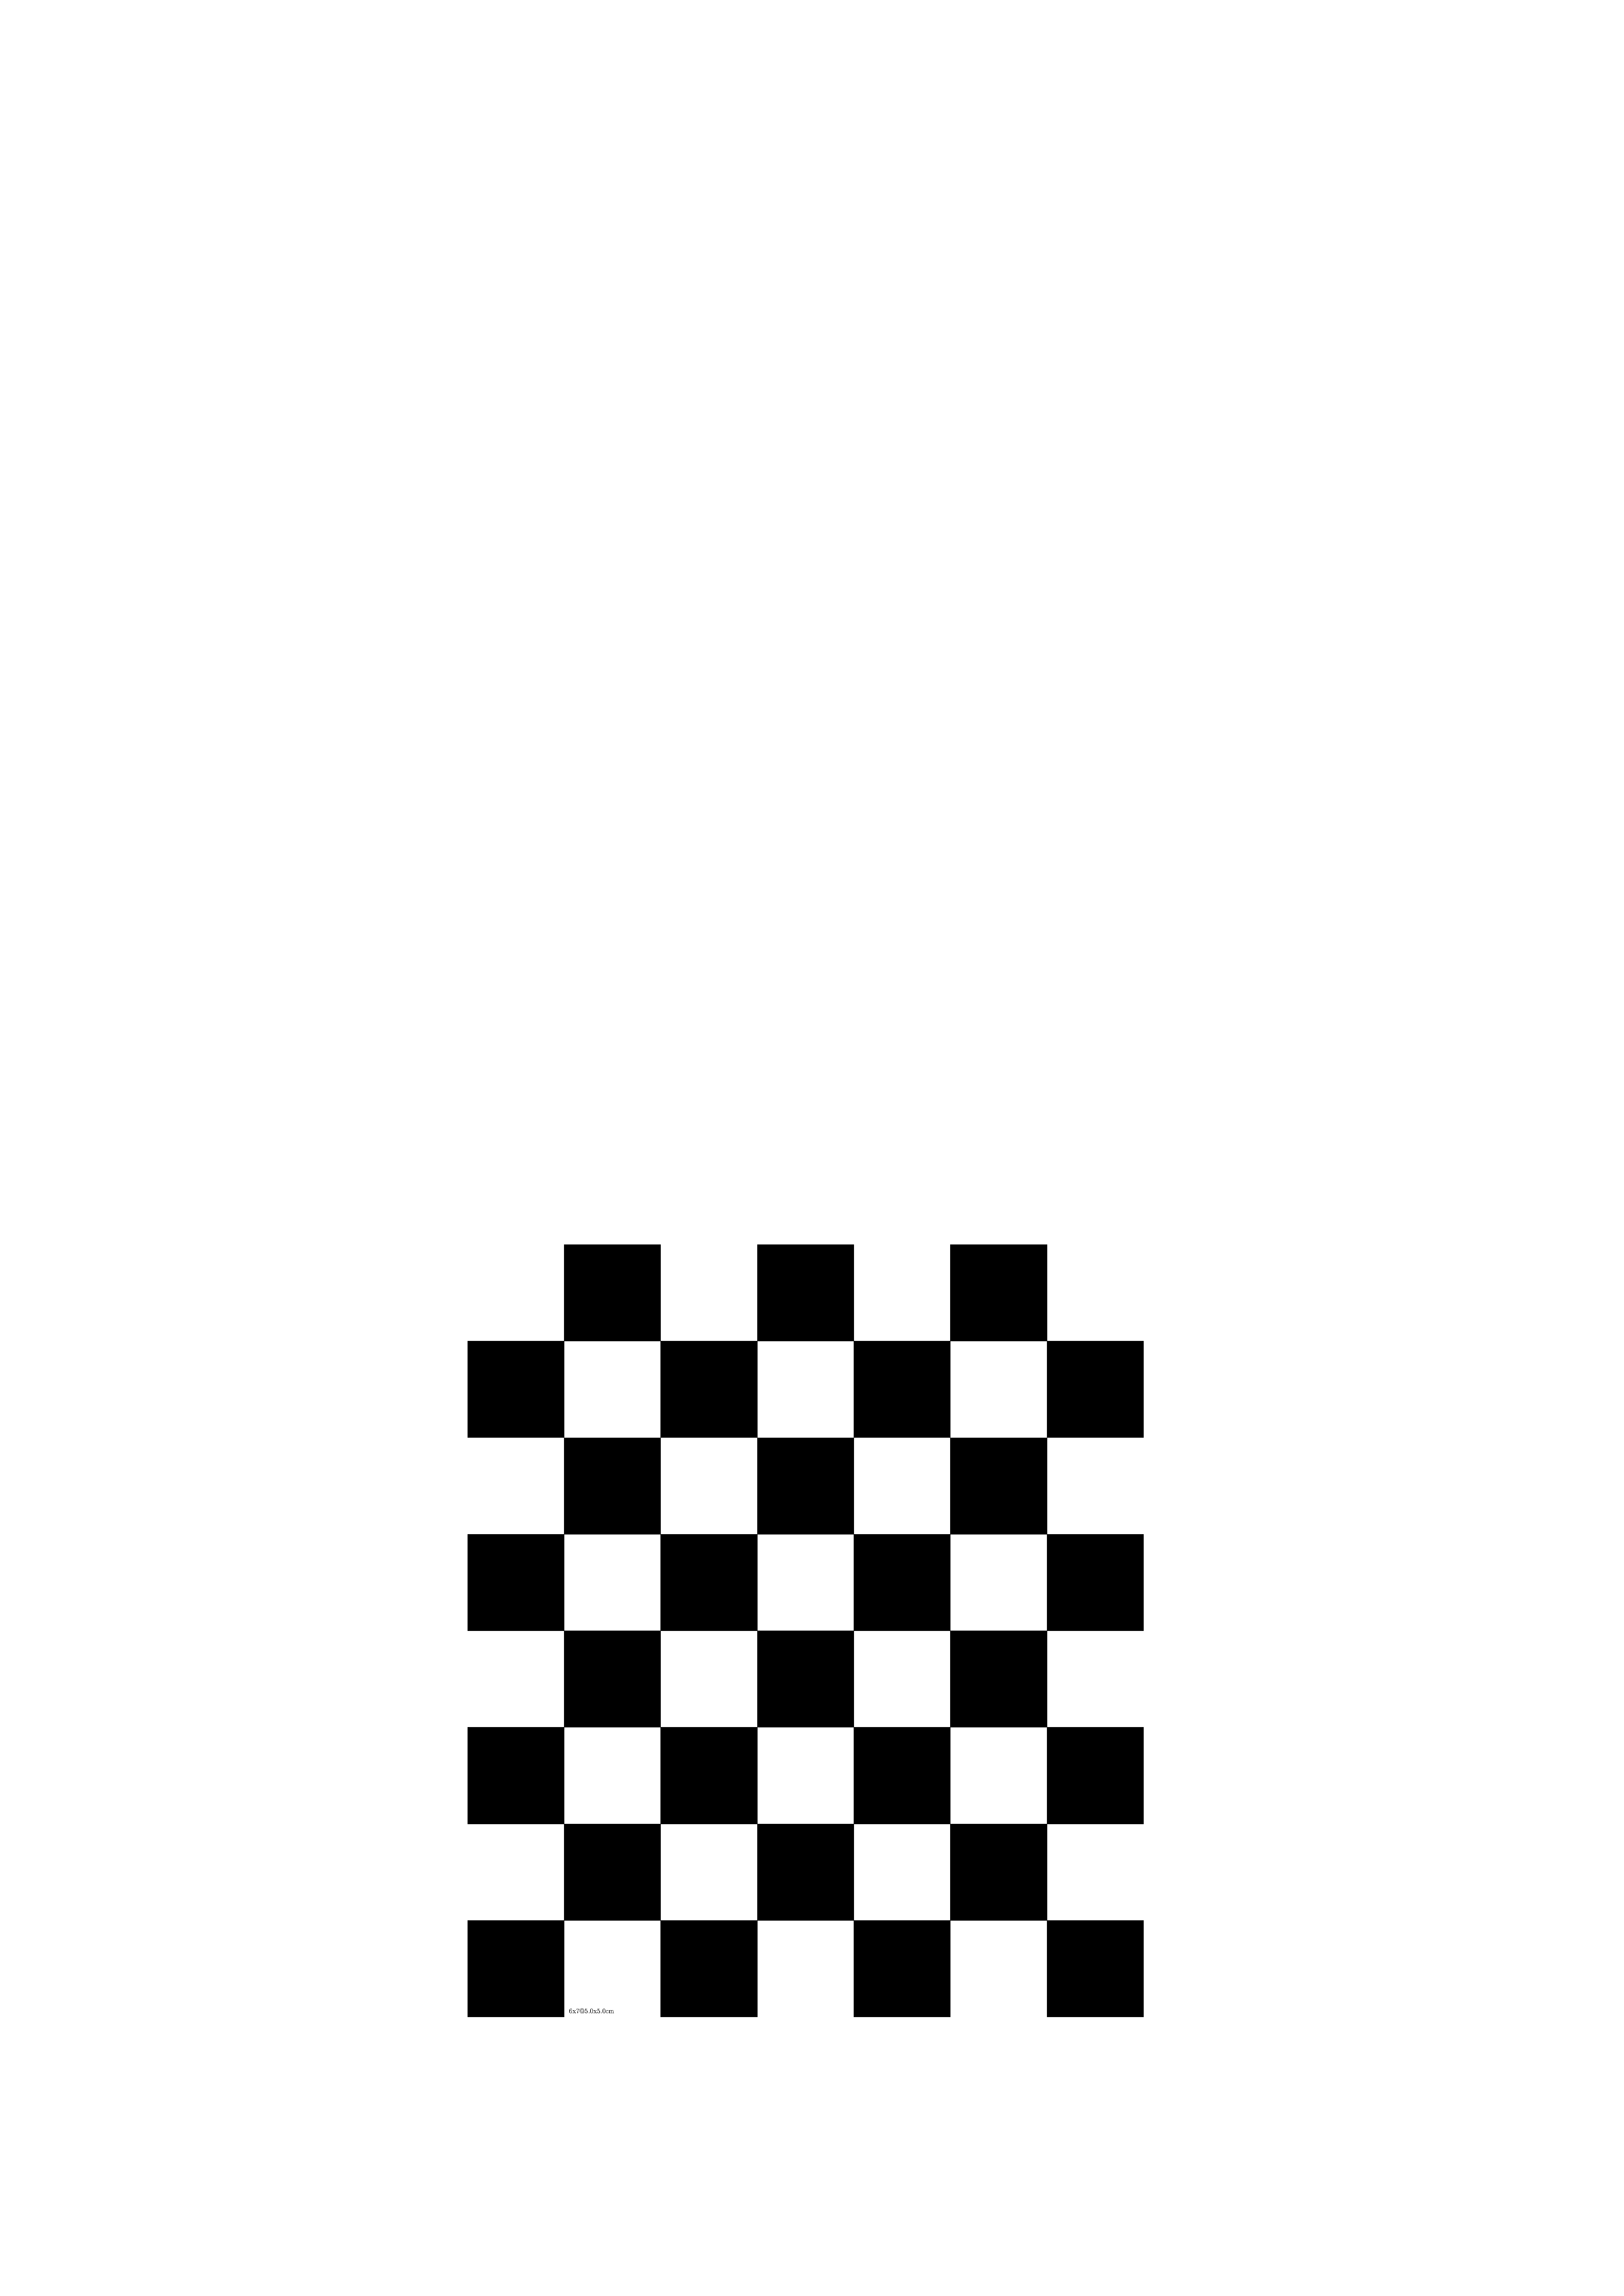
\includegraphics[width=0.2\textwidth]{figures/chapter2/fig2_11}
	\caption{7×6棋盘格}\label{fig2_11}
\end{figure}
\begin{equation}
\label{eqn:2.51}
\begin{aligned}
	s \left[ \begin{array}{c}{u} \\ {v} \\ {1}\end{array}\right] 
	&= \bm{K} \left[ \begin{array}{llll}{\bm{r}_{1}} & {\bm{r}_{2}} & {\bm{r}_{3}} & \bm{t}\end{array}\right] \left[ \begin{array}{c}{X} \\ {Y} \\ {0} \\ {1}\end{array}\right]
	= \bm{K} \left[ \begin{array}{lll}{\bm{r}_{1}} & {\bm{r}_{2}} & \bm{t}\end{array}\right] \left[ \begin{array}{c}{X} \\ {Y} \\ {1}\end{array}\right] \\
	&= \bm{H} \left[ \begin{array}{c}{X} \\ {Y} \\ {1}\end{array}\right] 
\end{aligned}
\end{equation}
其中 $s $是尺度因子, $\bm{H} $是单应矩阵$\bm{H}=\bm{K} \left[ \begin{array}{lll}{\bm{r}_{1}} & {\bm{r}_{2}} & \bm{t}\end{array}\right]  $ 。

$\bm{H} $ 矩阵有八个未知数,棋盘格的每对对应角点能提供两个方程,因此至少需要四个对应角点就可以算出世界平面到像素平面的映射矩阵,即单应矩阵$\bm{H} $ 。

设$\bm{H}=[ \bm{h}_1 \quad \bm{h}_2 \quad  \bm{h}_3 ]=\lambda \bm{K}[ \bm{r}_1 \quad \bm{r}_2 \quad  \bm{t} ] $ ,由式(\ref{eqn:2.51})得,
\begin{equation}
\label{eqn:2.52}
\left\{
\begin{aligned}
\lambda &= \frac{1}{s} \\ 
\bm{r}_{1} &= \frac{1}{\lambda} \bm{K}^{-1} \bm{h}_{1} \\ 
\bm{r}_{2} &= \frac{1}{\lambda} \bm{K}^{-1} \bm{h}_{2}
\end{aligned}
\right.
\end{equation}
因为 $\bm{r}_1 $和$\bm{r}_2 $ 是旋转矩阵,所以  $\bm{r}_1 $和$\bm{r}_2 $ 正交,则
\begin{equation}
\label{eqn:2.53}
\left\{
\begin{aligned}
\bm{r}_{1}^{T} \bm{r}_{2}&=0 \\ 
\left\|\bm{r}_{1}\right\|&=\left\|\bm{r}_{2}\right\|=1
\end{aligned}
\right.
\end{equation}
由式(\ref{eqn:2.52})和(\ref{eqn:2.53})可得,
\begin{equation}
\label{eqn:2.54}
\left\{
\begin{aligned} 
\bm{h}_{1}^{T} \bm{K}^{-T} \bm{K}^{-1} \bm{h}_{2} &=0 \\ 
\bm{h}_{1}^{T} \bm{K}^{-T} \bm{K}^{-1} \bm{h}_{1} &=\bm{h}_{2}^{T} \bm{K}^{-T} \bm{K}^{-1} \bm{h}_{2}=1
\end{aligned}
\right.
\end{equation}

即一个单应性矩阵可以提供两个方程,内参矩阵中有5个参数,因此至少需要3个单应性矩阵才能求解内参矩阵 $\bm{K} $ 。所以至少需要在3个不同的位置拍3张图片才能完成标定任务。

为了便于计算,令
\begin{equation}
\label{eqn:2.55}
\begin{aligned}
\bm{B} &= \bm{K}^{-T}\bm{K}^{-1}
=\left[
\begin{array}{ccc}
B_{11} & B_{12} & B_{13} \\
B_{21} & B_{22} & B_{23} \\
B_{31} & B_{32} & B_{33}
\end{array}
\right]  \\
&=\left[
\begin{array}{ccc}
\frac{1}{\alpha^2} & -\frac{\gamma}{\alpha^2\beta} & \frac{v_0\gamma-u_0\beta}{\alpha^2\beta} \\
-\frac{\gamma}{\alpha^2\beta} & \frac{\gamma^2}{\alpha^2\beta^2}+\frac{1}{\beta^2} & -\frac{\gamma(v_0\gamma-u_0\beta)}{\alpha^2\beta^2}-\frac{v_0}{\beta^2} \\
\frac{v_0\gamma-u_0\beta}{\alpha^2\beta} & -\frac{\gamma(v_0\gamma-u_0\beta)}{\alpha^2\beta^2}-\frac{v_0}{\beta^2} & \frac{(v_0\gamma-u_0\beta)^2}{\alpha^2\beta^2}+\frac{v_0}{\beta^2}+1
\end{array}
\right]
\end{aligned}
\end{equation}
注意,$\bm{B}$是一个对称矩阵,其有效元素为6个,将这6个元素写成向量的形式,
\begin{equation}
\label{eqn:2.56}
\setlength{\abovedisplayskip}{6pt}
\setlength{\belowdisplayskip}{6pt}
\bm{b} =\left[\begin{array}{ccc}B_{11} ,B_{12} , B_{22},B_{13},B_{23},B_{33}\end{array}\right]
\end{equation}
令$\bm{h}_i $ 为 $\bm{H} $的第 $i$  个列向量,则 
\begin{equation}
\label{eqn:2.57}
\setlength{\abovedisplayskip}{6pt}
\setlength{\belowdisplayskip}{6pt}
\bm{h}_i = [h_{i1},h_{i2},h_{i3}]^T
\end{equation}
所以,
\begin{equation}
\label{eqn:2.58}
\bm{h}_i \bm{K}^{-T}\bm{K}^{-1} \bm{h}_j = \bm{h}_i \bm{B} \bm{h}_j = \bm{v}_{ij}^T \bm{b}
\end{equation}
其中,
\[
\setlength{\abovedisplayskip}{6pt}
\setlength{\belowdisplayskip}{6pt}
\begin{aligned}
\bm{v}_{ij} = 
& \left[ \begin{array}{cccccc} 
h_{i1}h_{j1} & h_{i1}h_{j2}+h_{i2}h_{j1} & h_{i2}h_{j2} & h_{i3}h_{j1}+h_{i1}h_{j3} & h_{i3}h_{j2}+h_{i2}h_{j3} & h_{i3}h_{j3} 
\end{array} \right]^T
\end{aligned}
\]
进一步,由式(\ref{eqn:2.51})可推得,
\begin{equation}
\label{eqn:2.59}
\left\{
\begin{aligned} 
\bm{v}_{22}^T \bm{b} &= 0 \\ 
\bm{v}_{11} \bm{b} &= \bm{v}_{12} \bm{b} 
\end{aligned}
\right.
\end{equation}
写成矩阵形式,
\begin{equation}
\label{eqn:2.60}
\left[ 
\begin{array}{c} \bm{v}_{12}^T \\ \bm{v}_{11}-\bm{v}_{22} \end{array}
\right] \bm{b}  = 0
\end{equation}
这是一张棋盘格图像得到的约束等式,当有 $n$  张图像时,
\begin{equation}
\label{eqn:2.61}
\setlength{\abovedisplayskip}{6pt}
\setlength{\belowdisplayskip}{6pt}
\bm{Vb} = 0
\end{equation}
其中,$\bm{V} $ 是一个 $2n \times 6 $的矩阵, $\bm{b} $ 是一个6维列向量,所以,当有三张或者三张以上棋盘格图像时,就可以计算得到$\bm{B} $ ,进而得到相机的内参数矩阵 $\bm{K} $。

以上结果是在理想情况下推导得出的,但是现实中往往存在高斯噪声,所以为了增加标定结果的可靠性,使用MLE(Maximum Likelihood Estimation)来优化上面计算的结果。假设相机从不同的角度采集了$n$ 张包含棋盘格的图像,每张图像里有$m$ 个棋盘格角点。设第$i$ 张图像上的第 $j$个角点的三维点为$\bm{M}_{ij} $ ,则	
\begin{equation}
\label{eqn:2.62}
\setlength{\abovedisplayskip}{6pt}
\setlength{\belowdisplayskip}{6pt}
\hat{m}( \bm{K},\bm{R}_i,\bm{t}_i,\bm{M}_{ij}) = \bm{K}\bm{T}\bm{M}_{ij}
\end{equation}
其中,$\hat{m}( \bm{K},\bm{R}_i,\bm{t}_i,\bm{M}_{ij} )  $ 表示$\bm{M}_{ij} $ 对应的图像角点, $\bm{R}_i,\bm{t}_i $表示相机拍摄第  $i$ 张图像时的旋转和平移,$\bm{K} $ 是相机内参矩阵,角点$m_{ij} $ 的概率密度函数是:
\begin{equation}
\label{eqn:2.63}
f(m_{ij})=\frac{1}{\sqrt{2\pi}}e^{\frac{-(\hat{m}( \bm{K},\bm{R}_i,\bm{t}_i,\bm{M}_{ij} )^2}{\sigma^2}}
\end{equation}
构造似然函数:
\begin{equation}
\label{eqn:2.64}
L(\bm{K},\bm{R}_i,\bm{t}_i,\bm{M}_{ij}  ) = \prod^{n,m}_{i=1,j=1}f(m_{ij})=\frac{1}{\sqrt{2\pi}}e^{\frac{-\sum^n_{i=1}\sum^m_{j=1}(\hat{m}( \bm{K},\bm{R}_i,\bm{t}_i,\bm{M}_{ij} )^2}{\sigma^2}}
\end{equation}
让$L $ 取得最大值,需要最小化下面的式子:
\begin{equation}
\label{eqn:2.65}
\sum^n_{i=1}\sum^m_{j=1} \| \hat{m}( \bm{K},\bm{R}_i,\bm{t}_i,\bm{M}_{ij} )-m_{ij} \|^2
\end{equation}
针对这个最优解问题,可以使用LM(Levenberg-Marquardt)方法\upcite{more1978levenberg}求。

值得注意的是,“张正友标定法”只考虑了影响最大的径向畸变,且只用了前两个畸变参数,即式(\ref{eqn:2.12})中的 $k_1,k_2 $,
\begin{equation}
\label{eqn:2.66}
\left\{
\begin{aligned}
\hat{x} &= x + x[k_1(x^2 + y^2) + k_2(x^2 + y^2)^2] \\
\hat{y} &= y + y[k_1(x^2 + y^2) + k_2(x^2 + y^2)^2]
\end{aligned}
\right.
\end{equation}
其中, $(x,y)$和$(\hat{x},\hat{y}) $ 分别是畸变前和畸变后归一化成像平面的坐标。

设 $(u,v)$和$(\hat{u},\hat{v}) $ 分别是畸变前和畸变后的像素坐标,式(\ref{eqn:2.8})中的 $\gamma = 0 $ ,则,
\begin{equation}
\label{eqn:2.67}
\left\{
\begin{aligned}
\hat u &= u + (u-c_x)[k_1(x^2+y^2)+k_2(x^2+y^2)^2] \\
\hat u &= u + (u-c_y)[k_1(x^2+y^2)+k_2(x^2+y^2)^2]
\end{aligned}
\right.
\end{equation}
将式(\ref{eqn:2.67})写成矩阵形式:
\begin{equation}
\label{eqn:2.68}
\left[
\begin{array}{cc}
(u-c_x)(x^2+y^2) & (u-c_x)(x^2+y^2)^2 \\
(v-c_y)(x^2+y^2) & (v-c_y)(x^2+y^2)^2
\end{array}
\right]
\left[
\begin{array}{c}
k_1 \\ k_2
\end{array}
\right]=
\left[
\begin{array}{c}
\hat u -u \\ \hat v -v
\end{array}
\right]
\end{equation}

式(\ref{eqn:2.68})是从一张图像上的一个角点得到的,假设相机从不同的角度采集了 $n$ 张包含棋盘格的图像,每张图像里有 $m$个棋盘格角点,那么总共可以得到 $2mn$个等式,记作,
\begin{equation}
\label{eqn:2.69}
\bm{Dk} = \bm{d}
\end{equation}
可以得到,
\begin{equation}
\label{eqn:2.70}
\bm{k}=[k_1\ k_2]^T = (\bm{D}^T \bm{D})^{-1} \bm{D}^T\bm{d}
\end{equation}
同样,使用最大似然估计求最优解,使用LM方法最小化下面的式子求取参数,
\begin{equation}
\label{eqn:2.71}
\sum^n_{i=1}\sum^m_{j=1} \| \hat{m}( \bm{K},\bm{k},\bm{R}_i,\bm{t}_i,\bm{M}_{ij}  )-m_{ij} \|^2
\end{equation}

本系统使用的灰点相机标定出的内参和畸变结果如下:
\[
\bm{K}=
\left[\begin{array}{ccc}
{f_x} & {0}   & {c_x} \\
{0}   & {f_y} & {c_y} \\
{0}   & {0}   & {1}
\end{array}\right]
=
\left[\begin{array}{ccc}
{1066.015725} & {0}   & {474.867131} \\
{0}   & {1066.986974} & {300.515111} \\
{0}   & {0}   & {1}
\end{array}\right]
\]
\[
\bm{k} =
\left[\begin{array}{cc}
{k_1} & {k_2}   
\end{array}\right]^T
=
\left[\begin{array}{cc}
{-0.171420} & {0.210863}   
\end{array}\right]^T
\]
\subsection{IMU标定}
\label{chap:2.2.2}
在2.1.3小节研究了IMU的噪声模型,也就是加速度计和陀螺仪的高斯白噪声$\mathbf{n}_a $ $\mathbf{n}_w $和 ,以及bias  $\mathbf{b}_{a_t} $和$\mathbf{b}_{w_t} $ 。需要标定的就是这四个值。

通常用Allan方差来分析IMU的噪声模型\upcite{vagner2012experience},以陀螺仪为例,Allan方差可以分析如图\ref{fig2_12}所示的五种典型误差。加速度噪声模型分析同理,不再累述。
\begin{figure}[h]\setlength{\belowcaptionskip}{-12pt}
	\centering
	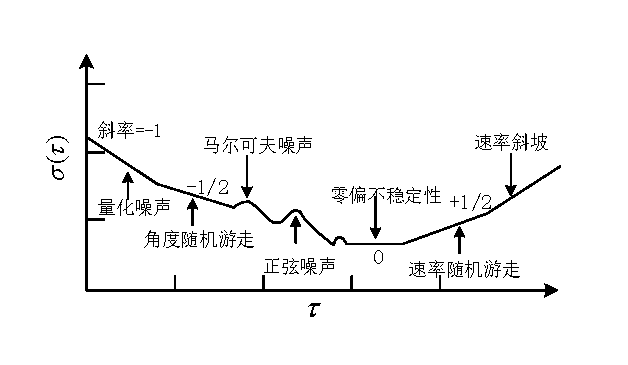
\includegraphics[width=0.5\textwidth]{figures/chapter2/fig2_12}
	\caption{Allan方差分析图}\label{fig2_12}
\end{figure}

首先区分几个比较复杂的概念,在2.1.3小节中说的白噪声 $\mathbf{n}_w, \mathbf{n}_a $通常在IMU使用手册中被描述为角度随机游走和速度随机游走,这是因为对角速度(加速度)的白噪声进行积分就是角度随机游走(速度随机游走)。也有的IMU手册中叫角速度噪声密度和加速度噪声密度,甚至直接简称为噪声密度。

角速率随机游走就是2.1.3小节中说的bias(随机游走) $\mathbf{b}_{w} $。一般IMU手册上不直接给出bias,而是给出bias (in)stability,即零偏(不)稳定性。因为在实践中,bias在长时间的积分中不会表现出真正的随机游走特性。bias (in)stability的值可以近似地表示bias的精度。在实践中,可以根据白噪声的大小以及bias (in)stability的值来确定bias的合理值。

Allan 方差可以分析任何信号,以确定潜在噪声过程的特征。信号的Allan方差是平均时间的函数。对于平均时间 $t$ ,Allan方差计算如下:

(1)获取一长串数据并将其按时间分成  $n$ 个长度为  $t$ 的区间。$n \geqslant 9 $ (否则得到的结果开始失去其意义)。

(2)求取每个区间中的数据的平均值得到平均值列表 $\left(a(t)_{1}, a(t)_{2}, \ldots, a(t)_{n}\right) $ 。 

(3)通过下面的式子计算Allan方差: 
\begin{equation}
\label{eqn:2.72}
\setlength{\abovedisplayskip}{6pt}
\setlength{\belowdisplayskip}{6pt}
\operatorname{AVAR}(t)=\frac{1}{2 \cdot(n-1)} \sum_{i}\left(a(t)_{i+1}-a(t)_{i}\right)^{2}
\end{equation}

为了分析噪声特性,需要计算Allan标准差:
\begin{equation}
\label{eqn:2.73}
\setlength{\abovedisplayskip}{6pt}
\setlength{\belowdisplayskip}{6pt}
\mathrm{AD}(t)=\sqrt{\mathrm{AVAR}(t)}
\end{equation}

在对数标度上绘制Allan标准差曲线(对数-对数AD曲线)。不同类型的随机噪声过程导致具有不同梯度的斜率。此外,不同的随机噪声过程通常出现在 $t$ 的不同区域中,从而可以容易地分辨出他们。确定随机噪声过程之后,可以直接从图中读取其数值参数。对于需要的白噪声,bias(随机游走)以及bias instability(零偏稳定性)可以通过下面的方式读取:

 (1) 对数-对数AD曲线上出现白噪声的地方的斜率为-1/2,通过在斜率上拟合直线并在$t=1$ 处读取。
 
 (2) 对数-对数AD曲线上出现bias(随机游走)的地方的斜率为+1/2,通过在斜率上拟合直线并在$t=3$ 处读取。
 
 (3) 对数-对数AD曲线上出现bias instability(零偏稳定性)的地方是曲线最小值附近的平坦区域,通过读取曲线上的最低点得到。

在IMU静止状态下采集四个小时的数据,然后绘制陀螺仪和加速度计的Allan方差曲线,如图\ref{fig2_13}和图\ref{fig2_14}所示。并将分析结果展示在表\ref{tab2.5}中,其中Gyr\_n和Acc\_n表示噪声项,Gyr\_w和Acc\_w表示随机游走。
\begin{figure}[!h]\setlength{\belowcaptionskip}{-12pt}
	\centering
	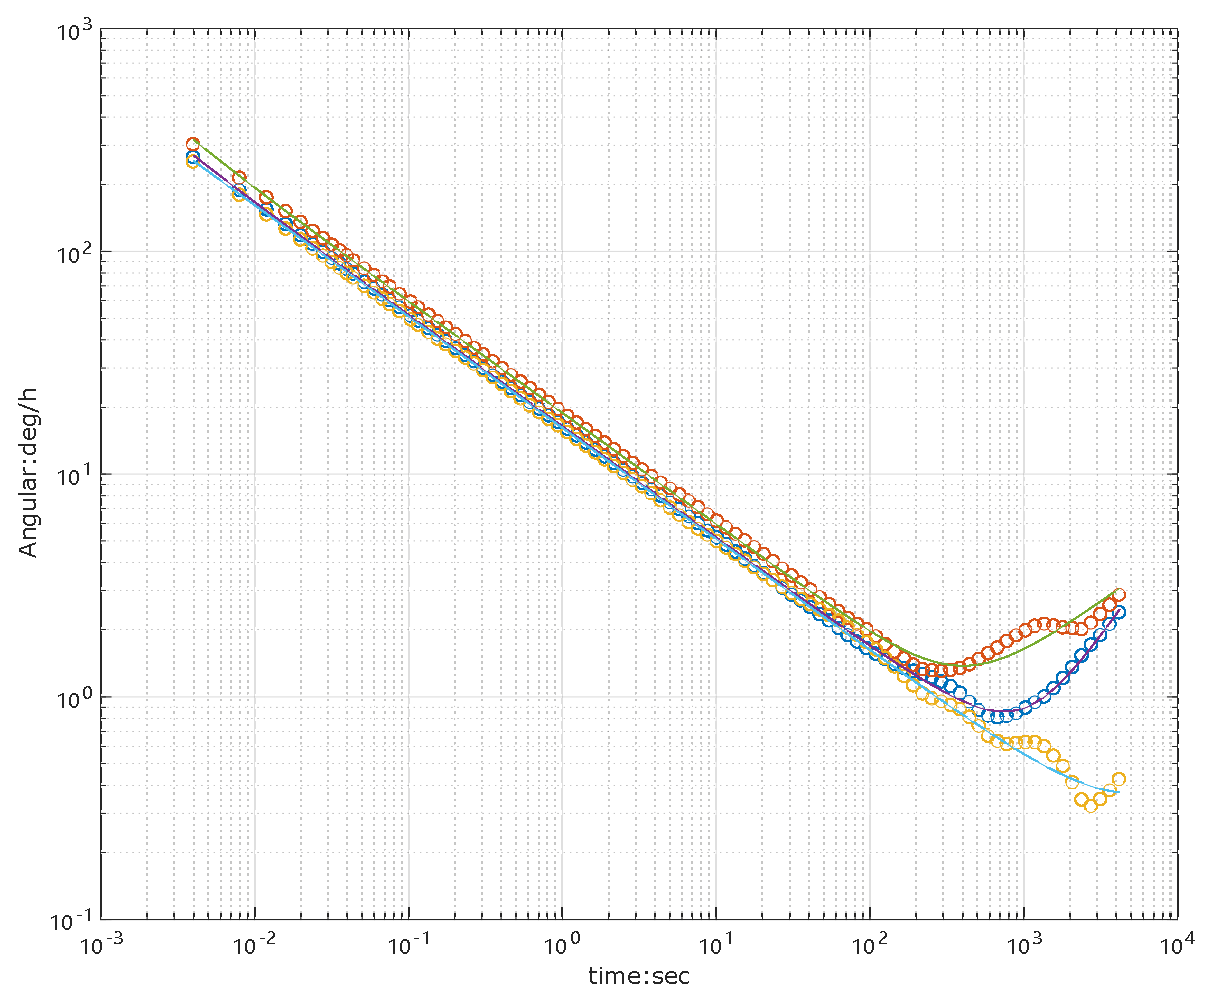
\includegraphics[width=0.8\textwidth]{figures/chapter2/fig2_13}
	\caption{陀螺仪Allan方差曲线}\label{fig2_13}
\end{figure}

\begin{figure}[!h]\setlength{\belowcaptionskip}{-12pt}
	\centering
	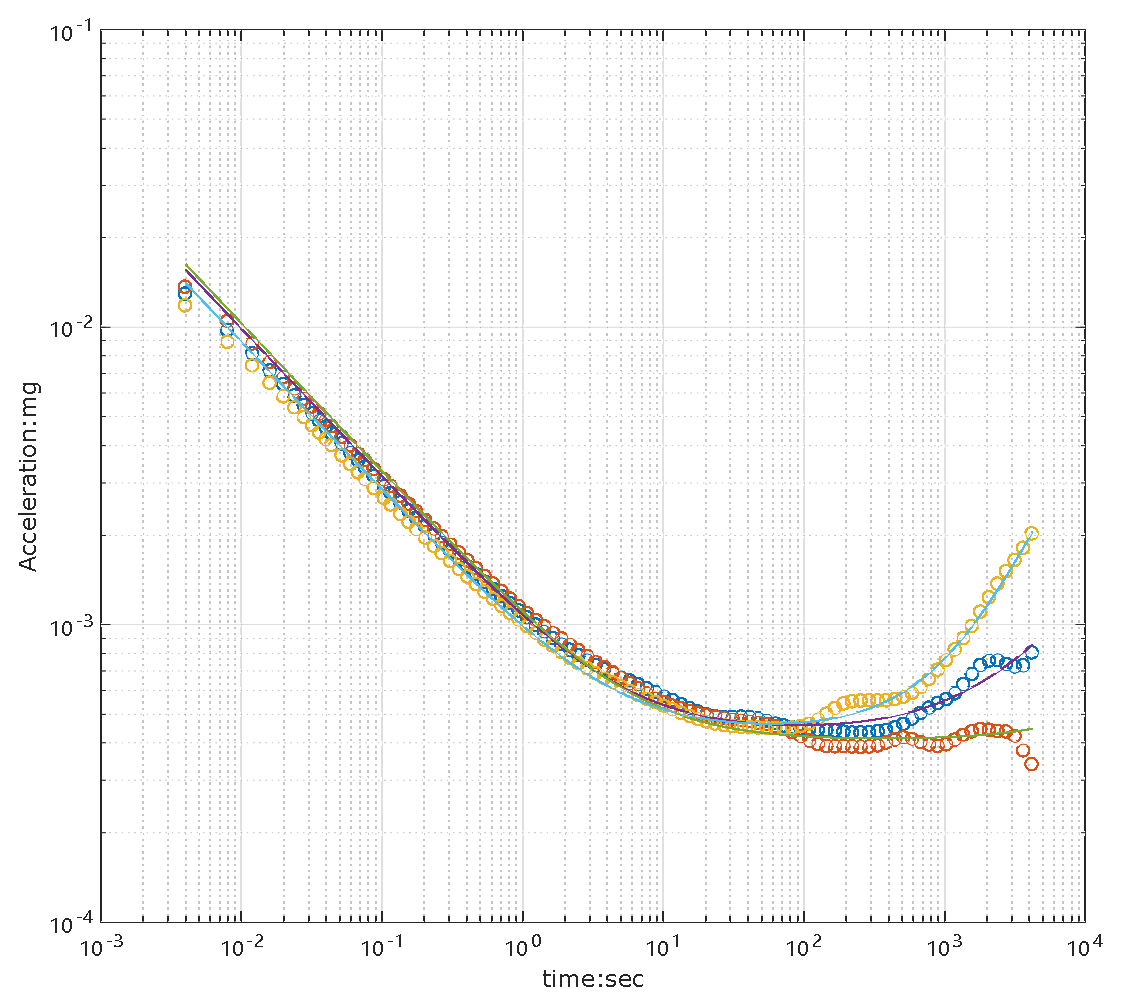
\includegraphics[width=0.8\textwidth]{figures/chapter2/fig2_14}
	\caption{加速度计Allan方差曲线}\label{fig2_14}
\end{figure}
\begin{table}[h]\setlength{\abovecaptionskip}{6pt}
	\zihao{5}  
	\centering
	\caption{IMU标定结果} \label{tab2.5}
	\begin{tabular*}{0.9\textwidth}{@{\extracolsep{\fill}}ccccc}
		\toprule
					&X轴		&Y轴	  &Z轴	&平均值 \\
		\midrule
		Gyr\_n (rad/s)	&1.25251e-03	&1.44058e-03	&1.23255e-03	&1.30854e-03\\
		Gyr\_w (rad/s)	&4.15778e-06	&6.66752e-06	&1.79872e-06	&4.20800e-06\\
		Acc\_n ($m/s^2$)	&1.70161e-02	&1.74575e-02	&1.56289e-02	&1.67009e-02\\
		Acc\_w ($m/s^2$)	&4.58804e-04	&4.14023e-04	&4.63646e-04	&4.45491e-04\\		
		\bottomrule
	\end{tabular*}
\end{table}
\subsection{同步与联合标定}
在视觉和IMU融合系统中,保证二者在时间上的同步非常重要。因为在初始化的时候需要将IMU预积分的值与视觉的观测值进行对齐,从而恢复单目视觉的尺度、重力的方向以及其它初始化参数。只有保证了正确的初始值,才能确保后端非线性优化能够收敛到一个最优值。而IMU和视觉对齐的程度完全取决于时间戳的匹配精准度。为了尽可能的对齐相机和IMU的时间戳,对传感器进行硬件同步。

本文选用的灰点相机拥有外部触发模式,也就是能够通过外部脉冲来触发相机进行曝光。选用的IMU能够向外输出与自己等采样频率的方波。如图\ref{fig2_15}所示,进行硬件同步的思路是:将IMU输出的方波(250Hz)通过硬件分频电路十分频,然后送到相机的触发端口(25Hz)进行触发曝光。

硬件同步为接下来的相机/IMU联合标定奠定了基础。
\begin{figure}[h]\setlength{\belowcaptionskip}{-12pt}
	\centering
	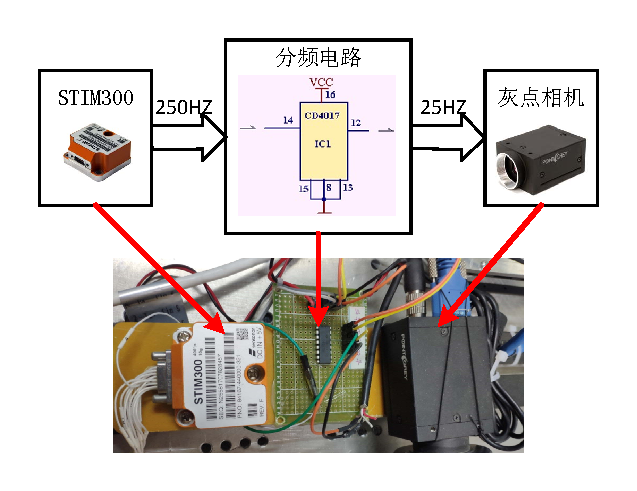
\includegraphics[width=0.45\textwidth]{figures/chapter2/fig2_15}
	\caption{硬件同步示意图}\label{fig2_15}
\end{figure}

使用开源的视觉/惯性标定工具:kalibr\upcite{furgale2012continuous}\upcite{furgale2013unified}进行联合标定。联合标定需要动态标定,需要的输入文件包括:相机内参及畸变参数,IMU噪声参数,带IMU信息的视频以及标定板信息。其中,相机内参和IMU噪声参数是\ref{chap:2.2.1}和\ref{chap:2.2.2}小节标定出来的结果。视频是在不同角度下拍摄的标定板图像,需要注意的是,在拍摄视频时需要激活IMU所有的轴向信息(包括偏航、横滚和俯仰)。采用的标定板和传统标定相机的棋盘格标定板(图\ref{fig2_11})不一样,是Aprilgrid标定板,如图\ref{fig2_16}所示。Aprilgrid标定板能够给出序号信息,可以避免姿态计算出现跳跃的情况。视IMU坐标系和载体坐标系重合,相机和IMU的坐标系定义如图\ref{fig2_17}所示。
\begin{figure}[h]\setlength{\belowcaptionskip}{-12pt}
	\centering	
	\begin{minipage}[t]{0.35\linewidth}				
		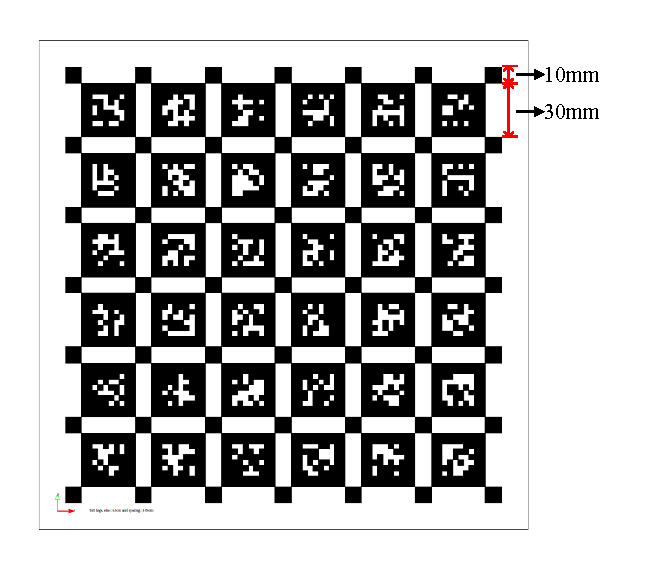
\includegraphics[height=4.5cm,width=6cm]{figures/chapter2/fig2_16}		
		\caption{Aprilgrid标定板}	\label{fig2_16}	
	\end{minipage}%	
	\hspace{0.1in}	
	\begin{minipage}[t]{0.5\linewidth}		
		\centering		
		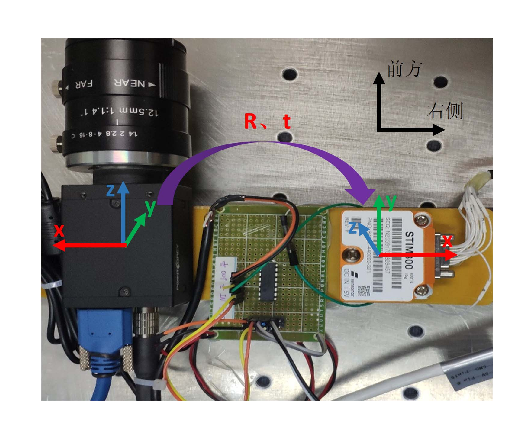
\includegraphics[height=4.5cm,width=6.5cm]{figures/chapter2/fig2_17}		
		\caption{相机和IMU的坐标系定义} \label{fig2_17}		
	\end{minipage}	
\end{figure} 

联合标定主要标定如下参数:

(1)  T\_ic:与IMU的外参。即相机到IMU的变换矩阵。

(2)  tmeshift:相机与IMU之间的时间偏移。这个值可以反应出时间同步的精度,timeshift越小表明同步效果越好。

(3)  Gravity vector:重力矢量。重力的大小能够反映出标定的精度。

另外,kalibr还会给出加速度和角速度的误差图,用来评估IMU的精度,以及相机重投影误差,可以用来评估的标定结果。

表\ref{tab2.6}是的相机和IMU联合标定的结果。可见相机和IMU之间的平移在10cm左右,这符合本系统实际安装距离。时间偏移约为9ms。重力大小是9.8$m/s^2$ 。可见,标定出的结果较为可靠。
\begin{table}[h]\setlength{\abovecaptionskip}{6pt}
	\zihao{5}  
\newcommand{\tabincell}[2]{\begin{tabular}{@{}#1@{}}#2\end{tabular}}  %导言区
	\centering
	\caption{联合标定结果} \label{tab2.6}
	\begin{tabular*}{0.75\textwidth}{@{\extracolsep{\fill}}cc}
		\toprule
		T\_ic			& $\left[ \begin{array}{cccc}
			0.99956 & 0.02956 & 0.00015 & 0.10048 \\ 
			 0.00028 & -0.00458 & -0.99999 & 0.01208 \\ 
			-0.02955 & 0.99955 & -0.00459 & -0.07922 \\ 
			{0} & {0} & {0} & 1
		\end{array}\right]$\\
		\midrule
		\tabincell{c}{Timeshift(s)}            &   -0.009307066448628993 \\
	    \midrule
		\tabincell{c}{Gravity vector($m/s^2$)}            &   [ 0.12538627\ \  -9.80181878\ \   -0.27757847] \\
		\bottomrule
	\end{tabular*}
\end{table}

图\ref{fig2_18}是IMU角速度误差和加速误差。可见,角速度误差在±0.04$rad/s$ 范围内波动,加速度误差在0.5$m/s^2$ 范围内波动。

图\ref{eqn:2.19}是相机的重投影误差。可见,重投影误差在±0.8个像素单位波动。这表明相机内参和畸变参数标定的很准确。
\begin{figure}[!h]\setlength{\belowcaptionskip}{-12pt}
	\centering
	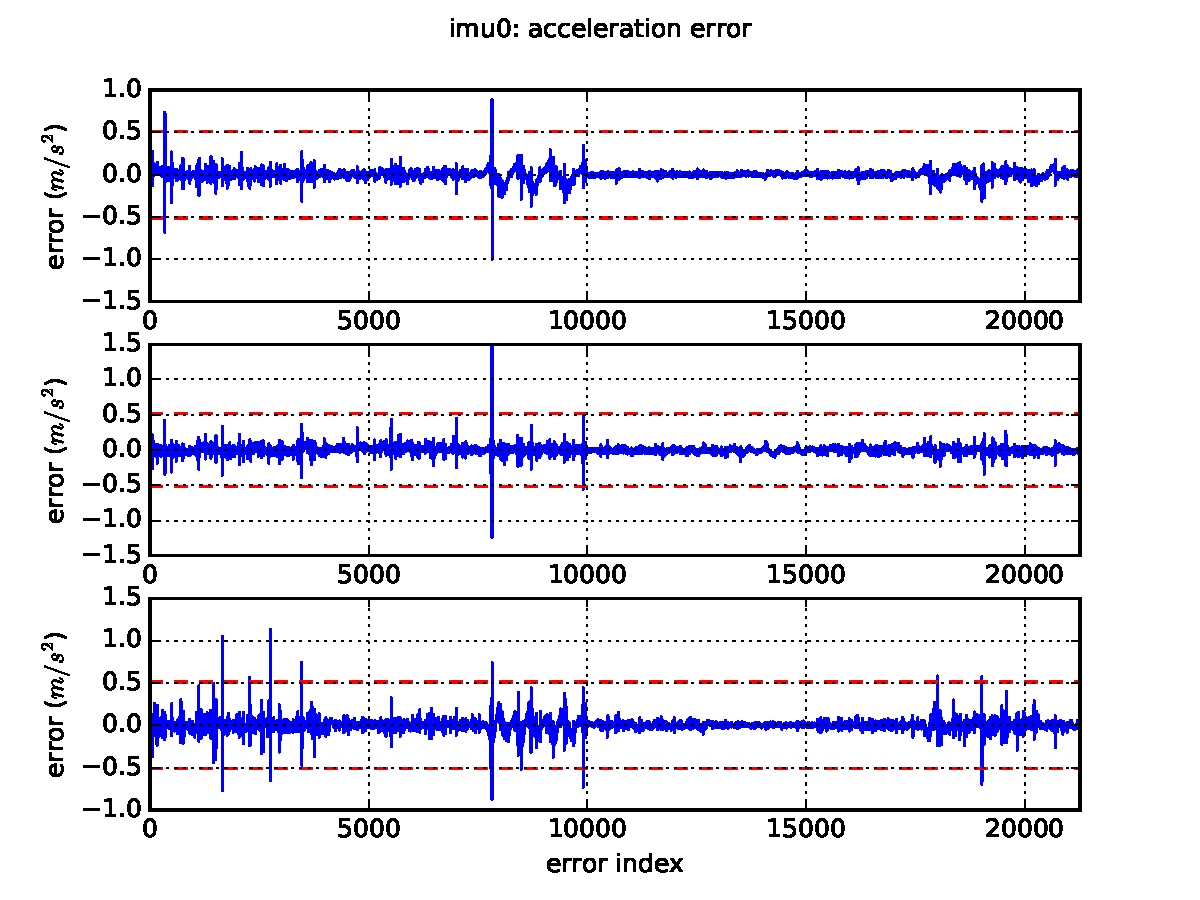
\includegraphics[width=0.47\textwidth]{figures/chapter2/fig2_18(a)}
	\hspace{0.01cm}
	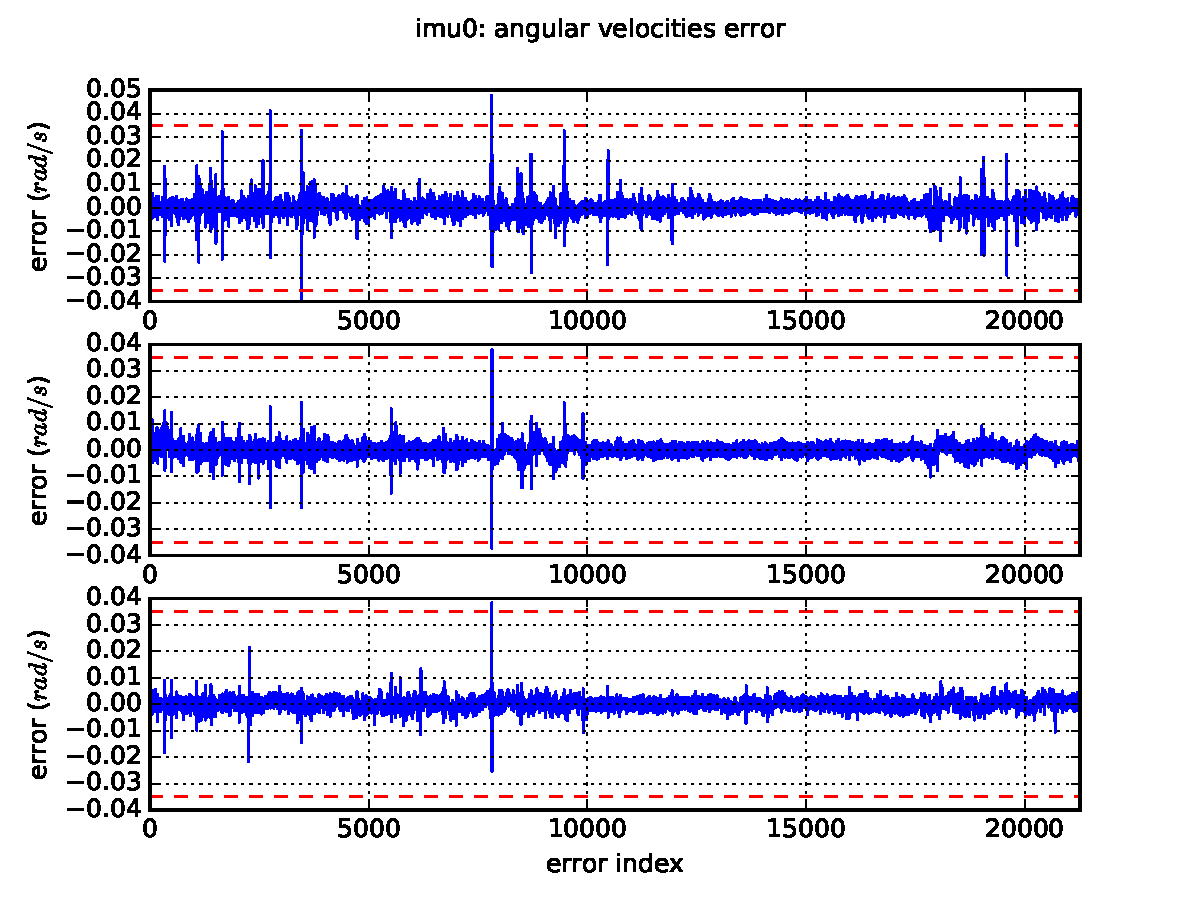
\includegraphics[width=0.47\textwidth]{figures/chapter2/fig2_18(b)}
	\caption{IMU角速度误差和加速误差}
	\label{fig2_18}
\end{figure}
\begin{figure}[!h]\setlength{\belowcaptionskip}{-12pt}
	\centering
	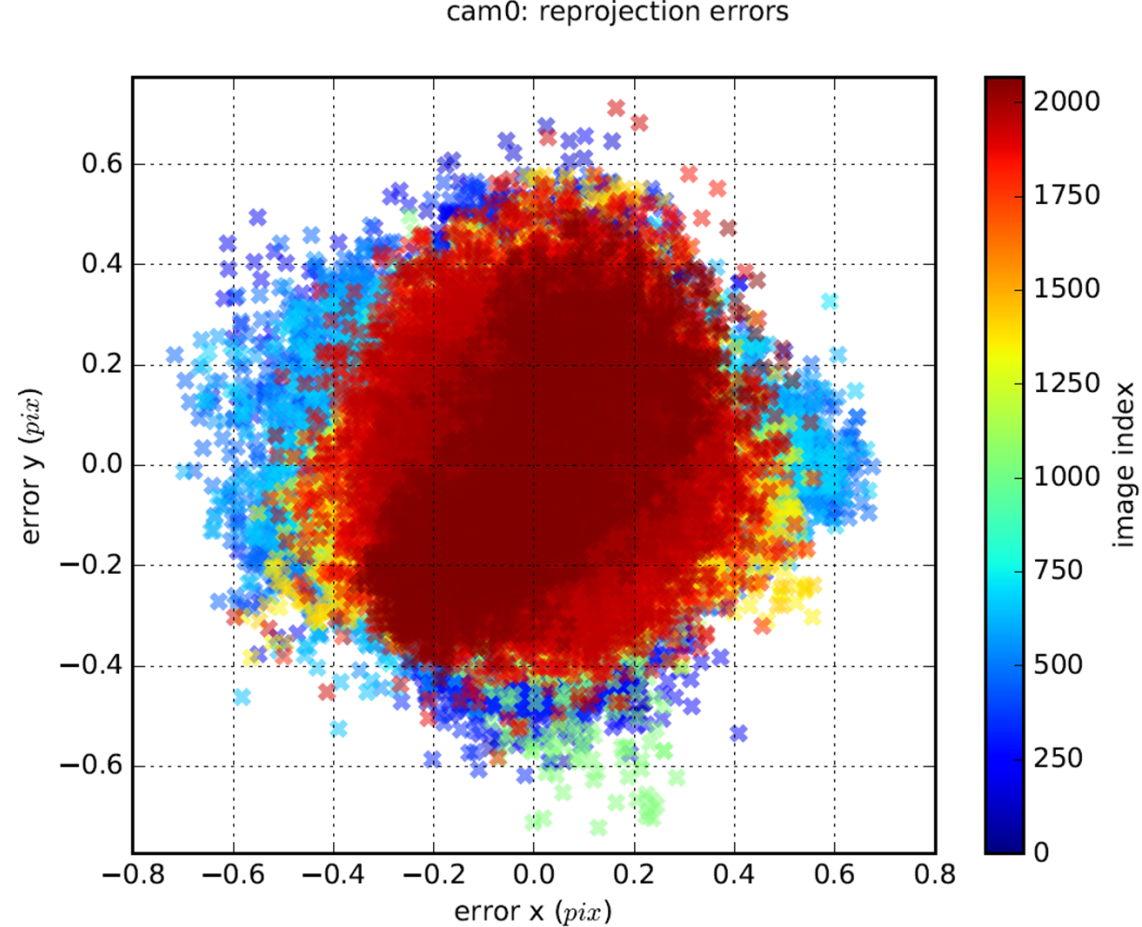
\includegraphics[width=0.6\textwidth]{figures/chapter2/fig2_19}
	\caption{相机重投影误差}\label{fig2_19}
\end{figure}
\section{硬件组建与ROS信息采集}
\subsection{硬件组建}
本系统的硬件系统构成如图\ref{fig2_20}所示。
\begin{figure}[h]\setlength{\belowcaptionskip}{-12pt}
	\centering
	\includegraphics[width=0.6\textwidth]{figures/chapter2/fig2_20}
	\caption{硬件系统构成}\label{fig2_20}
\end{figure}

图中\mycircled{1}是灰点单目相机(配镜头),\mycircled{2}是IMU(STIM300),\mycircled{3}是磁力计,\mycircled{4}是RTK,\mycircled{5}是12v锂电池,\mycircled{6}是稳压模块,\mycircled{7}是RS232串口转USB,\mycircled{8}是相机和IMU的同步电路,\mycircled{9}是Intel NUC处理器,\mycircled{10}是磁力计和底座连接的连接杆,\mycircled{11}是底座。其中,RTK不属于多传感器融合系统,主要用他来采集差分GPS信号,将GPS的轨迹当作真实值并和本系统输出轨迹作比较,方便分析系统的定位精度。为了避免载体(汽车)本身对磁力计的干扰,将磁力计用\mycircled{10}架高,相对于底座的高度为60cm。而且为了尽量避免铁磁性物体对磁场的干扰,硬件系统的底座以及连接杆都是铝制的。
\subsection{ROS信息采集}
ROS(Robot Operating System)译作机器人操作系统\upcite{Fairchild2016ROS},通常应用在机器人上,它操作简单,功能强大,尤其适用于向机器人这种多任务、多节点的复杂环境。ROS的功能非常丰富,本文不打算一一介绍,只对其通信机制中的“话题”作简要研究。

在ROS中,一个节点(Node)就是一个可执行文件。由于机器人的模块众多,通常不会将所有的模块放在一个节点中实现,而是一个节点实现一个模块。比如,节点1用来驱动相机获取图像,节点2用来驱动电机控制机器人移动,节点3用来接收图像并进行定位……这样以来可以降低系统的崩溃频率,使程序便于维护。
在ROS的众多通信方式中,话题(topic)是最常用的一种。话题适合处理类似传感器信息这样的实时性、周期性的消息。话题是一种节点与节点之间的单向异步通信方式。发布节点(Publisher Node)发布话题到节点管理器Master,订阅节点从Master订阅话题。订阅节点接收到话题消息后会触发回调函数,在回调函数里对话题消息进行处理。

如\ref{fig2_21}所示,使用节点1采集相机图像,话题为/camera/image\_raw;节点2采集IMU数据,话题为/imu\_data;节点3采集磁力计数据,话题为/dmc\_data;节点4采集RTK数据,话题为/rtk\_data。节点5,6,7分别代表前端、后端和回环。节点1$\sim$ 4采集到的传感器数据将被以话题的形式发布到节点管理器Matser,然后节点5,6,7都可以独立的订阅所有话题,并在自己的回调函数进行处理,各个节点互不干扰,独立运行,这就是话题单向异步通信的优势。值得称赞的是,使用ROS采集传感器信息的时候可以将所有话题记录下来,之后可以像回放视频那样重复播放,达到重复使用数据的效果。
\begin{figure}[h]\setlength{\belowcaptionskip}{-12pt}
	\centering
	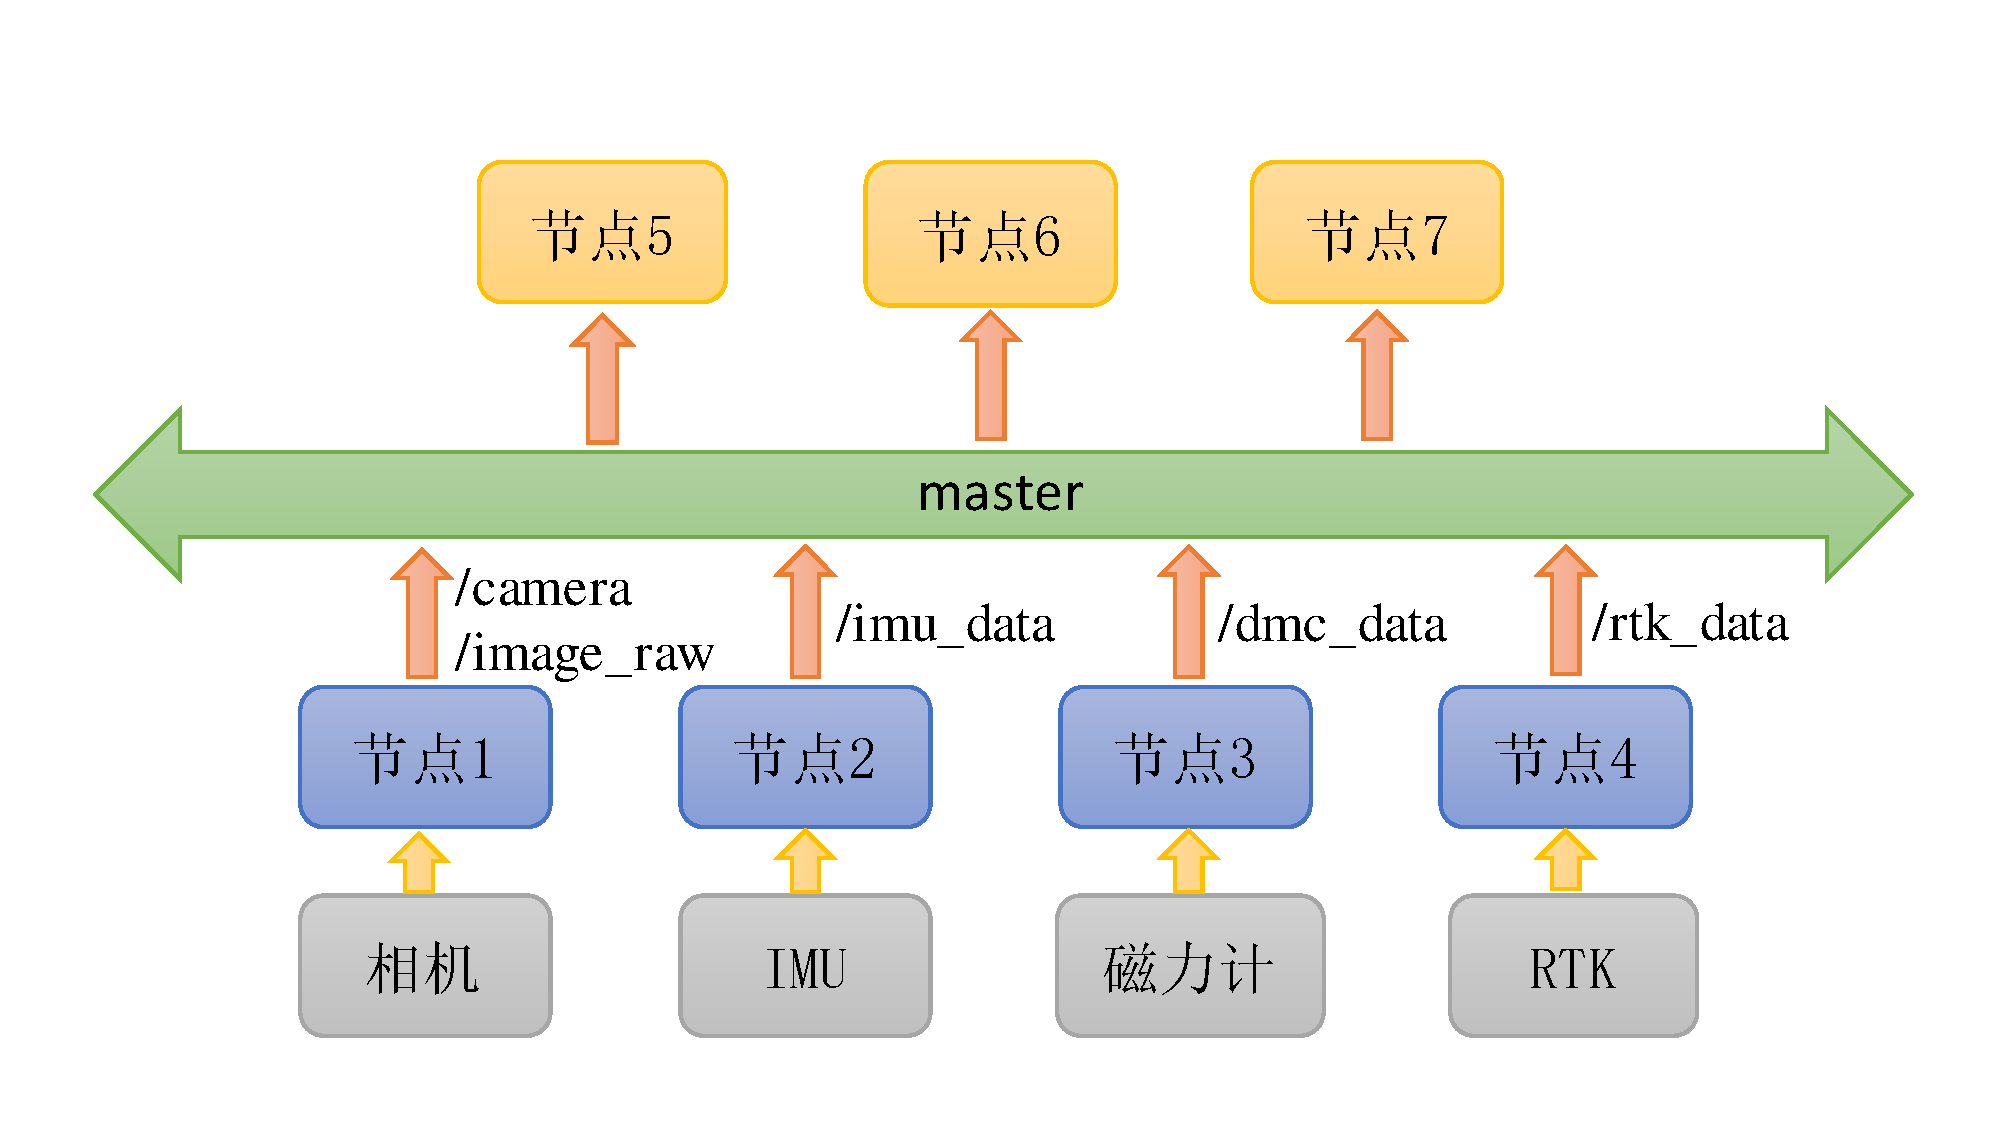
\includegraphics[width=0.6\textwidth]{figures/chapter2/fig2_21}
	\caption{ROS采集传感器信息及同通信示意图}\label{fig2_21}
\end{figure}
\section{本章小结}
本章主要研究系统的硬件部分,包括传感器模型及其选型,传感器标定与同步,以及硬件系统搭建和传感器信息采集。对传感器的数学模型进行了详细的推导,并详细研究了传感器的标定原理和步骤。完善可靠的硬件系统是后续进行算法研究和实验验证的基础。
\chapter{系统前端及初始化}
\label{chap:3}
本章主要研究系统的前端和初始化相关内容,其中前端主要包括视觉信息预处理和IMU预积分,视觉信息预处理包括特征提取和跟踪,异常点剔除。初始化主要包括多视图几何基础,visual初始化,以及Visual-IMU联合初始化。
\section{视觉信息预处理}
在视觉SLAM中,前端也称为视觉里程计(Visual Odometer,VO)\upcite{高翔2017视觉}。VO的实现方法有很多,包括特征点法,直接法和光流法。特征点法需要提取特征点,这包括提取关键点和计算描述子,然后进行特征匹配;直接法是从光流法继承而来的,不需特征提取及匹配;光流法不进行特征点匹配,取而代之的是利用光流跟踪特征点。表\ref{tab:3.1}列出了三种方法的优缺点。综合考虑,本文选用光流法作为视觉前端算法。
\begin{table}[h]\setlength{\abovecaptionskip}{6pt} 
	\zihao{5}  
	\centering
	\caption{特征点法、直接法和光流法对比} \label{tab:3.1}
	\begin{tabular}{m{0.1\textwidth}<{\centering} m{0.22\textwidth}<{\centering}  m{0.24\textwidth}<{\centering} m{0.26\textwidth}<{\centering} }%
		\toprule
		优缺点	   &   特征点法   &  	直接法	  &   光流法 \\
		\midrule
		优点	   &(1)对比直接法和光流法,鲁棒性高;(2)不受照影响。&(1)不需要特征点提取和匹配,计算量小;(2)可以在无纹理或者重复纹理场景下工作;(3)可以构建半密集或密集地图。 &(1)不需要计算描述子和匹配特征,计算量小;(2)可以在无纹理或者重复纹理场景下工作;(3)容易移植到嵌入式系统中,方便IMU进行融合;(4)可以构建半密集或者密集的地图。 \\
		缺点 &(1)在无纹理或者重复纹理场景下无法工作;(2)计算量大,不能保证实时性;(3)仅用CPU无法构建半稠密或稠密地图。  &(1)基于灰度不变假设,对光照变化敏感;(2)单个像素没有区分度,需要计算像素块;(3)图像是非凸的,容易产生局部极值。&(1)基于灰度不变假设,对光照变化敏感;\\	
		\bottomrule
	\end{tabular}
\end{table} 

\subsection{关键点和关键帧}
关键点也可以称为角点,它与特征点的区别是它没有描述子。常用的角点检测算法有Harris角点\upcite{harris1988combined}和FAST角点\upcite{rosten2006machine}。相比于Harris角点,FAST角点检测速度更快,因为FAST角点不需要计算像素的梯度,仅仅通过比较周围像素的亮度来确定是否为角点。如图\ref{fig3_1},它的算法流程如下:

(1)选取图像中的一个像素 $p$ ,设其亮度为 $I_p $ ;

(2)设定一个合适的亮度阈值 $T$ (例如设为 $I_p $ 的 20\%  );

(3)以像素  $p$  为圆心,画半径为3像素的圆,并选取圆上的所有像素(16个);

(4)如果在这16个像素点中,有连续 $N $  个点的亮度都大于$I_p+T $ 或者小于 $I_p-T $,那么像素 $p $ 就是角点。通常$N $  取12,9和11,分别称为FAST-12,FAST-9和FAST-11;

(5)对图像中的每一个像素执行以上步骤,提取所有的角点。
\begin{figure}[h]\setlength{\belowcaptionskip}{-12pt}
	\centering
	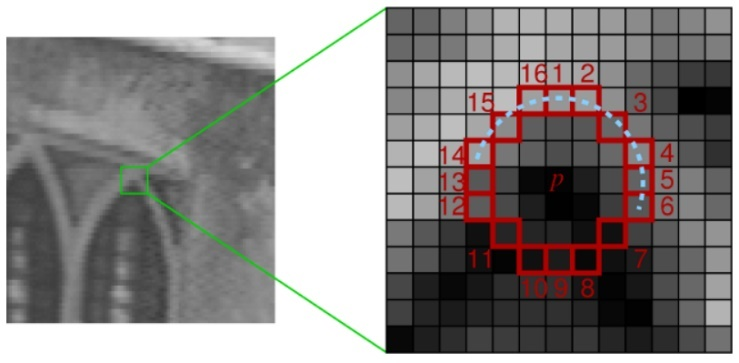
\includegraphics[width=0.5\textwidth]{figures/chapter3/fig3_1}
	\caption{FAST角点}\label{fig3_1}
\end{figure}

针对FAST-12算法,为了提高检测效率,可以添加一个预判别的操作,用来排除掉大部分不是角点的像素点。方法为:直接检测像素 $p$ 周围第1,5,9和13个像素点的亮度。当这四个像素中有三个像素的亮度同时大于$I_p+T $ 或者小于$I_p-T $ 时,该像素才有可能是角点,才会继续利用FAST-12进行角点检测,否则直接排除该像素。这样的预判别操作大幅度提升了角点检测的速度。

增加预判操作确实可以大大提高算法效率,但是到此为止算法还存在一个缺点,检测出来的很多相邻的角点挤在一起。为了消除这种邻近位置有多个角点重合的情况,需要进行非大极值抑制(Non-Maximal Suppression,NMS)\upcite{blaschko2011branch}。方法如下:

(1)计算每一个检测到的角点的响应值(score function) $V$,这里$V$ 定义为角点点 $p$ 和它邻域16个像素点的绝对差值之和,即,
\[
\setlength{\abovedisplayskip}{6pt}
\setlength{\belowdisplayskip}{6pt}
V = \Sigma_{x \in S} |I_{p\rightarrow x} - I_p|
\] 
其中 $S$ 表示16的邻域像素点的集合。

(2)考虑两个相邻的角点,并比较它们的 $V$ 值,并删除 $V$ 值较小的角点。
图\ref{fig3_2}展示了FAST角点提取。其中,(a)是原始图像,(b)是不加NMS 的FAST角点提取,(c)是加入NMS的FAST角点提取。
\begin{figure}[h]\setlength{\belowcaptionskip}{-12pt}
	\centering
	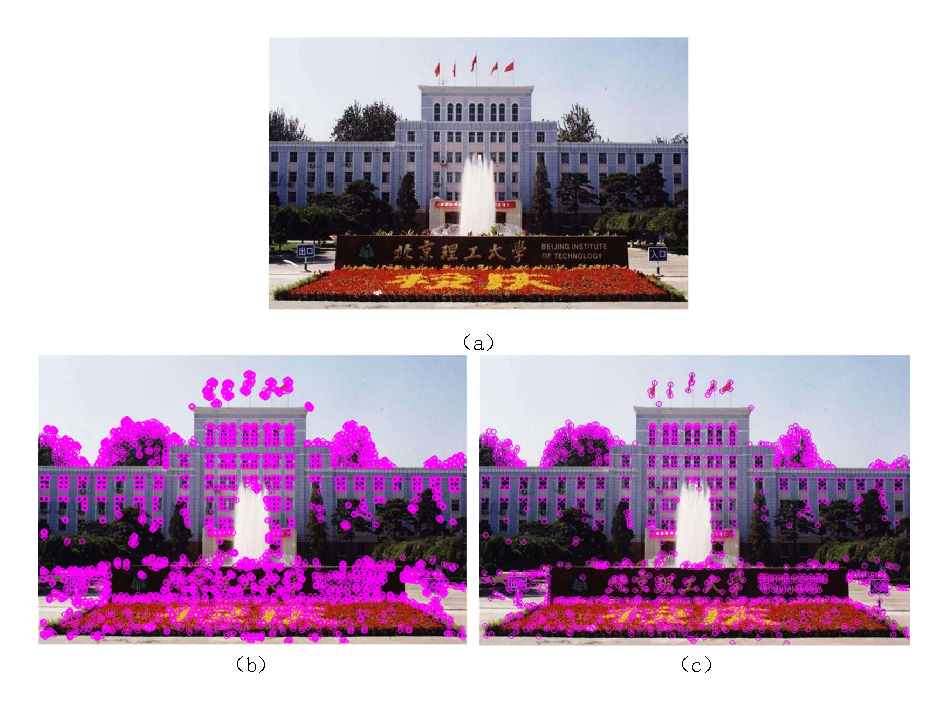
\includegraphics[width=0.9\textwidth]{figures/chapter3/fig3_2}
	\caption{(a)原始图像;(b)不加NMS 的FAST角点提取;(c)加入NMS的FAST角点提取。}\label{fig3_2}
\end{figure}

考虑到系统的实时性,不会对所有的图像都进行关键点提取,而是引入关键帧机制,即只对关键帧提取关键点,非关键帧则直接忽略。本文依据两个标准来选择关键帧。第一,两个关键帧之间要有足够的视差。当跟踪到的特征的平均视差介于当前帧和最近的关键帧视差之间,则将当前帧视为新的关键帧。第二,每张图像跟踪到的关键点要大于某一阈值,否则,将该帧视为关键帧。这样做是为了防止图像关键点完全跟丢,导致系统崩溃。
\subsection{特征跟踪}
关键点检测出来后就需要对其进行跟踪,本文采用光流跟踪关键点。光流是用来描述像素在图像中随着时间运动的方法,如图\ref{fig3_3}所示。跟踪部分像素的运动称为稀疏光流,跟踪所有像素的运动称为稠密光流。在SLAM中通常用LK(Lucas-Kanade)光流\upcite{bouguet2001pyramidal}来跟踪关键点的位置。
\begin{figure}[h]\setlength{\belowcaptionskip}{-12pt}
	\centering
	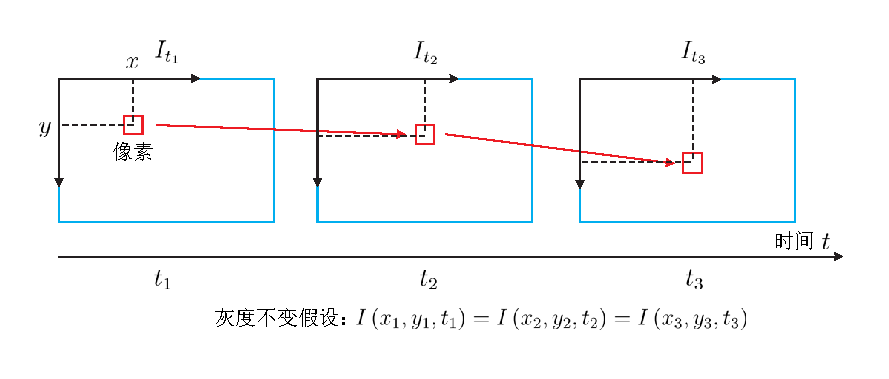
\includegraphics[width=0.8\textwidth]{figures/chapter3/fig3_3}
	\caption{LK光流法示意图}\label{fig3_3}
\end{figure}

在LK光流中,相机是运动的,也就是说相机的图像随着时间的变化而变化。所以,图像和时间之间存在一个映射关系:$\bm{I}(t) $ 。那么,在 $t$ 时刻,图像中 $(x,y)$ 处的像素的灰度可以记作:$ \boldsymbol{I}(x, y, t) $ 。这样,图像就是关于位置和时间的函数,该函数的值域就是图像的灰度。假设三维空间中的一个点 $p$ 在 $t$  时刻时的像素坐标为 $(x,y)$ 。随着时间的变化,$p$ 的像素坐标将发生变化。要估计出每一时刻该点的像素坐标。
首先,需要提出一个基本的假设:灰度不变假设。即三维空间中的点在每张图像中的像素灰度值是固定不变的。例如,在 $t+\mathrm{d} t $ 时刻点  $p$ 的像素坐标为 $(x+\mathrm{d} x, y+\mathrm{d} y) $ ,则,
\begin{equation}
\label{eqn:3.1}
\boldsymbol{I}(x+\mathrm{d} x, y+\mathrm{d} y, t+\mathrm{d} t)=\boldsymbol{I}(x, y, t)
\end{equation}
对式(\ref{eqn:3.1})左边用泰勒公式展开并保留一阶项,得,
\begin{equation}
\label{eqn:3.2}
\boldsymbol{I}(x+\mathrm{d} x, y+\mathrm{d} y, t+\mathrm{d} t) \approx \boldsymbol{I}(x, y, t)+\frac{\partial \boldsymbol{I}}{\partial x} \mathrm{d} x+\frac{\partial \boldsymbol{I}}{\partial y} \mathrm{d} y+\frac{\partial \boldsymbol{I}}{\partial t} \mathrm{d} t
\end{equation}
由式(\ref{eqn:3.1})和(\ref{eqn:3.2})得,
\begin{equation}
\label{eqn:3.3}
\frac{\partial \boldsymbol{I}}{\partial x} \mathrm{d} x+\frac{\partial \boldsymbol{I}}{\partial y} \mathrm{d} y+\frac{\partial \boldsymbol{I}}{\partial t} \mathrm{d} t=0
\end{equation}
\begin{equation}
\label{eqn:3.4}
\frac{\partial \boldsymbol{I}}{\partial x} \frac{\mathrm{d} x}{\mathrm{d} t}+\frac{\partial \boldsymbol{I}}{\partial y} \frac{\mathrm{d} y}{\mathrm{d} t}=-\frac{\partial \boldsymbol{I}}{\partial t}
\end{equation}
其中,$\mathrm{d} x / \mathrm{d} t $ 和 $\mathrm{d} y / \mathrm{d} t $ 分别表示像素在 $x$ 轴方向和 $y$ 轴方向上的速度分量,将其分别记为 $u, v $ 。$\partial \boldsymbol{I} / \partial x $ 和 $\partial \boldsymbol{I} / \partial y $ 表示 $x$ 轴方向和 $y$轴方向上的像素梯度,分别记为 $\boldsymbol{I}_{x}, \boldsymbol{I}_{y} $ 。$\partial \boldsymbol{I} / \partial t $ 表示图像灰度随时间的变化量,记为$\boldsymbol{I}_{t} $ 。这样可以将式(\ref{eqn:3.4})写成如下矩阵形式,
\begin{equation}
\label{eqn:3.5}
\left[ \begin{array}{ll}{\boldsymbol{I}_{x}} & {\boldsymbol{I}_{y}}\end{array}\right] \left[ \begin{array}{l}{u} \\ {v}\end{array}\right]=-\boldsymbol{I}_{t}
\end{equation}

假设在图像中的某一个 $w \times w $ 大小的窗口内所有的像素(共有 $w^2 $ 个)具有相同的运动,那么可以得到 $w^2 $ 个方程,
\begin{equation}
\label{eqn:3.6}
\left[ \begin{array}{cc}{\boldsymbol{I}_{x}} & {\boldsymbol{I}_{y}}\end{array}\right]_{k} \left[ \begin{array}{c}{u} \\ {v}\end{array}\right]=-\boldsymbol{I}_{t k}, \quad k=1, \ldots, w^{2}
\end{equation}
记,
\begin{equation}
\label{eqn:3.7}
A=\left[ \begin{array}{c}{\left[\boldsymbol{I}_{x}, \boldsymbol{I}_{y}\right]_{1}} \\ {\vdots} \\ {\left[\boldsymbol{I}_{x}, \boldsymbol{I}_{y}\right]_{k}}\end{array}\right], \boldsymbol{b}=\left[ \begin{array}{c}{\boldsymbol{I}_{t 1}} \\ {\vdots} \\ {\boldsymbol{I}_{t k}}\end{array}\right]
\end{equation}
所以,式(\ref{eqn:3.6})可以写为,
\begin{equation}
\label{eqn:3.8}
\boldsymbol{A} \left[ \begin{array}{l}{u} \\ {v}\end{array}\right]=-\boldsymbol{b}
\end{equation}
使用最小二乘法求解式(3.8),
\begin{equation}
\label{eqn:3.9}
\left[ \begin{array}{c}{u} \\ {v}\end{array}\right]^{*}=-\left(\boldsymbol{A}^{T} \boldsymbol{A}\right)^{-1} \boldsymbol{A}^{T} \boldsymbol{b}
\end{equation}

这样就可以计算处像素的运动速度 $u,v$ ,从而计算出像素在图像中的位置。也就实现了使用LK光流来跟踪角点的目的。
图\ref{fig3_4}是光流跟踪FAST角点示意图。其中,左图(a)中的点是检测到的FAST角点,右图(b)是相机向左平移一段距离拍摄的图像,蓝线是LK光流跟踪角点的轨迹。
\begin{figure}[h]\setlength{\belowcaptionskip}{-12pt}
	\centering
	\subfigure[FAST角点]{
		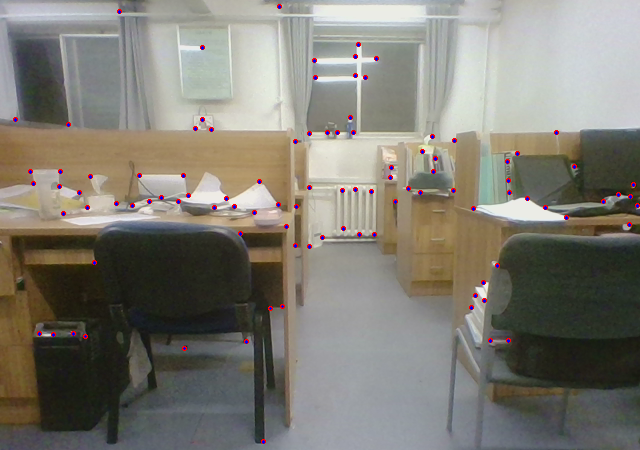
\includegraphics[width=0.4\textwidth]{figures/chapter3/LK1}}
	\subfigure[LK跟踪]{
		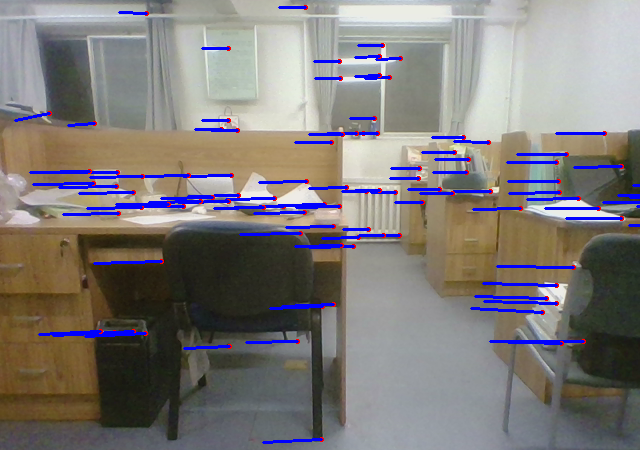
\includegraphics[width=0.4\textwidth]{figures/chapter3/LK2}}
	\caption{光流跟踪FAST角点}\label{fig3_4}
\end{figure}
\subsection{异常点剔除}
在视觉SLAM中,不管是特征点匹配还是光流跟踪都会出现误匹配或误跟踪的情况,那些匹配正确或者跟踪正确的点称为“局内点(inlier)”,而匹配错误或者跟踪错误的点称为“局外点(outlier)” 或者“异常点”。这些“异常点”会影响SLAM的定位精度,因此需要对其进行剔除。

在视觉SLAM中剔除“outlier”常用的方法是RANSAC(Random Sample Consensus),该算法是Fischler和Bolles等人于1981年最先提出的\upcite{fischler1981random2}。它可以得到有效的数据,即“局内点”,剔除无用数据,即“局外点”。在实践中,“异常点”通常是由于测量错误、假设错误和计算错误等原因造成,他们通常与正确数据“相距”很远。

该算法假设:

(1)样本数据集包含“局内点”和“局外点”;

(2)“局外点”不满足计算假设的数学模型;

(3)“局内点”满足某一数学模型,并可以计算其参数;

(4)其余数据是噪声数据。

该算法步骤如下:

(1)从样本数据集 $S$ 中随机选取一小组点集 $s$ (共有 $n$ 个),假设 $s$  的所有点为“局内点”,通过该点集得到一个数学模型 $F$ ;

(2)用该数学模型 $F$ 去测试 $S$ 中除 $s$ 外的其他点,并假设满足该数学模型的点为“局内点”;

(3)如果被假设为“局内点”的数量 $n$ 大于设定的阈值 $T$ ,那么就认为数学模型 $F$ 是合理的;

(4)用所有假设的“局内点”重新估计数学模型 ;

(5)如果迭代次数大于等于 $k$ ,则停止,否则重复上述步骤。

关键在于如何确定 $k$ 值。假设在样本数据集中“局内点”的概率是 $w $ ,则,
\begin{equation}
\label{eqn:3.10}
w = \frac{n_{inliers}}{n_{inliers} + n_{outliers}}
\end{equation}

最少需要假设 $n$ 个“局内点”确定模型 $F$ ,$n$ 视具体问题而定。$n$ 个假设的“局内点”都是实际的“局内点”的概率为 $w^n$ ,$n$ 个假设的“局内点”中至少有一个是实际的“局外点”的概率为 $1-w^n $ 。$k$ 次随机选取的点集 $s$ 中没有一次全部是“局内点”的概率是 $(1-w^n)^k $ ,用  $P$ 表示 $k$ 次随机选取的点集 $s$  中全部都是“局内点”的概率, $P$ 也表示取到正确解的概率或者置信度,则,
\begin{equation}
\label{eqn:3.11}
\setlength{\abovedisplayskip}{6pt}
\setlength{\belowdisplayskip}{6pt}
P=1-(1-w^n)^k
\end{equation}
“局内点”的概率 $w$  是一个先验值,可以根据先验假设一个初值。此时,可以计算出迭代次数 $k$  ,
\begin{equation}
\label{eqn:3.12}
k = \frac{log(1-P)}{log(1-w^n)}
\end{equation}
以上是“异常点”剔除的通用步骤,下面研究RANSAC是如何剔除关键点的。
以计算基本矩阵来剔除“异常点”为例,则上面研究的数学模型 $F$ 为基本矩阵。使用8点法计算 $F $ ,则 $n=8$ 。图\ref{fig3_5}展示了使用基本矩阵剔除异常点的步骤。
\begin{figure}[h]\setlength{\belowcaptionskip}{-12pt}
	\centering
	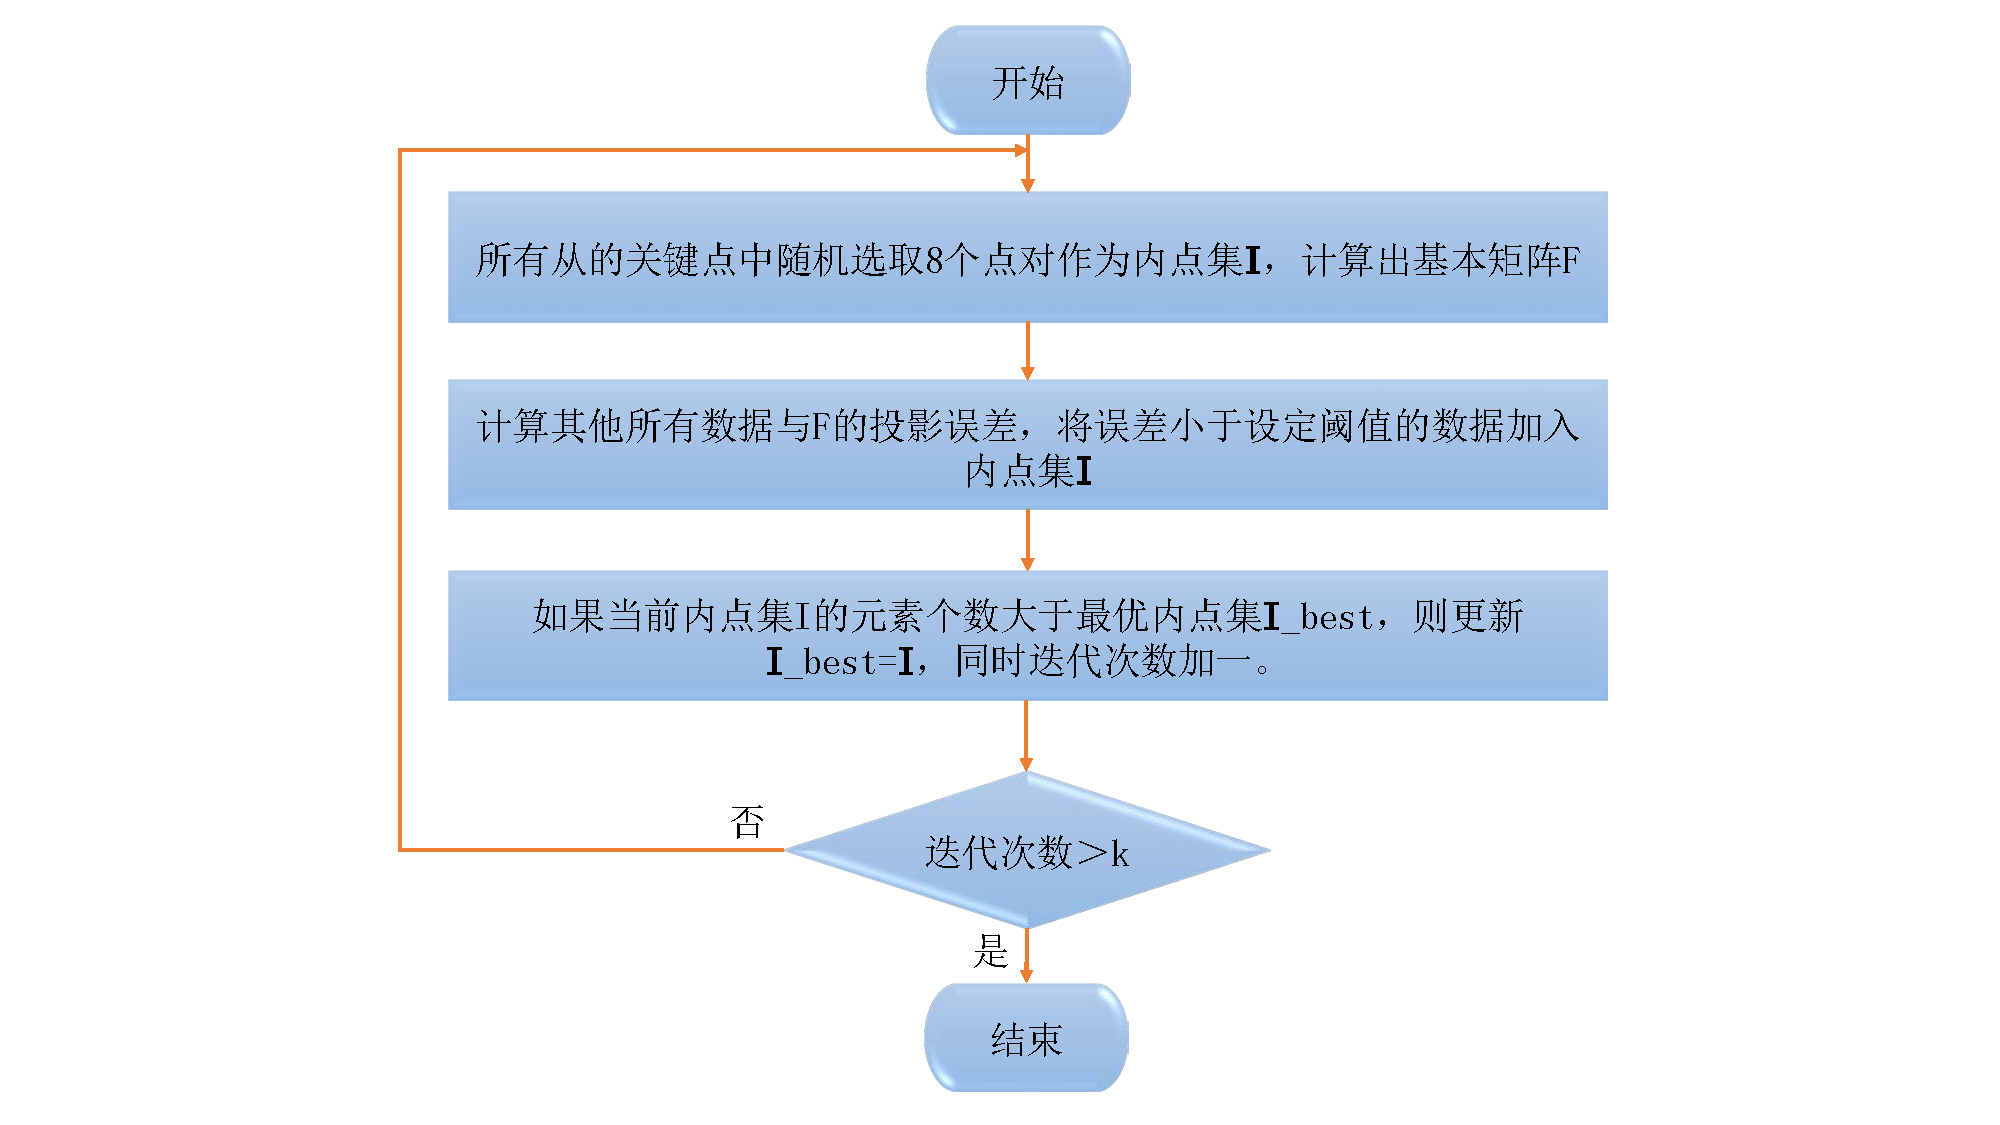
\includegraphics[width=0.65\textwidth]{figures/chapter3/fig3_5}
	\caption{用基本矩阵剔除异常点}\label{fig3_5}
\end{figure}

图\ref{fig3_6}是异常点剔除前后对比图。其中,图(a)是LK光流跟踪到的FAST角点(没有进行异常点剔除),总共1270个点;图(b)是经过异常点剔除后的跟踪的角点,总共775个点。
\begin{figure}[h]\setlength{\belowcaptionskip}{-12pt}
\centering
	\subfigure[剔除前]{
	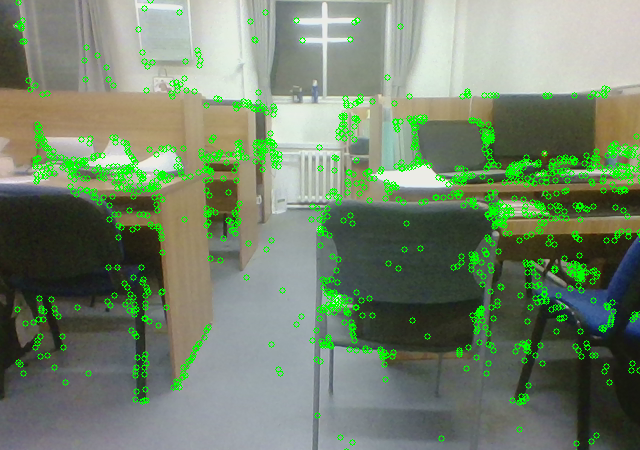
\includegraphics[width=0.4\textwidth]{figures/chapter3/RAN1}}
	\subfigure[剔除后]{
	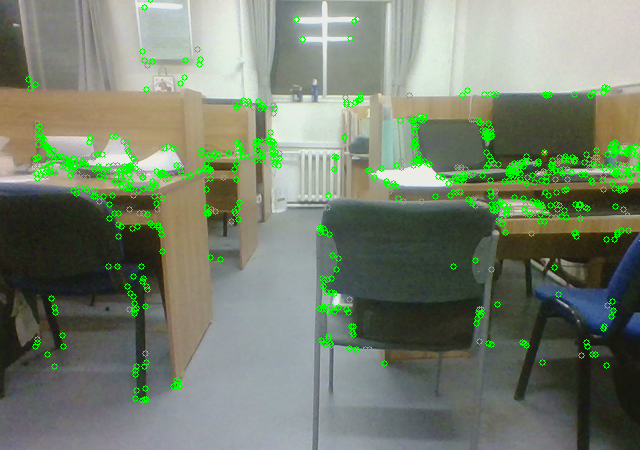
\includegraphics[width=0.4\textwidth]{figures/chapter3/RAN2}}
	\caption{异常点剔除}\label{fig3_6}
\end{figure}
\section{IMU预积分}
通常情况下,IMU的数据频率要远大于相机的数据频率,不可能计算每一个IMU时刻状态量,为了与视觉进行融合,需要提前对相邻视觉帧之间的IMU数据进行积分,这个步骤称为预积分\upcite{forster2015imu}\upcite{shen2015tightly}。图\ref{fig3_7}是预积分示意图。
\begin{figure}[h]\setlength{\belowcaptionskip}{-12pt}
	\centering
	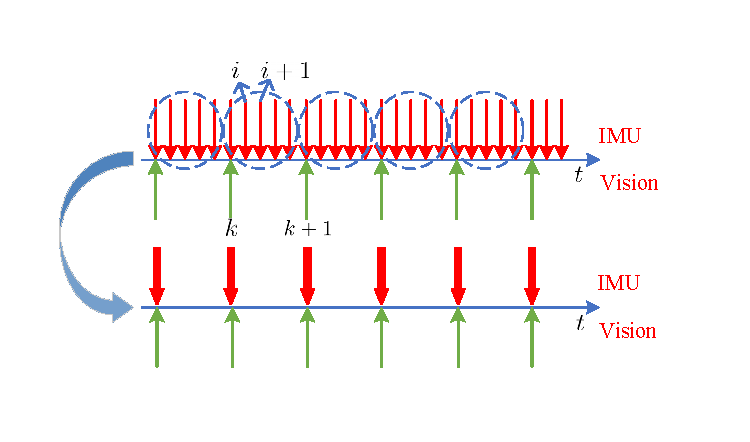
\includegraphics[width=0.3\textwidth, angle=-90]{figures/chapter3/fig3_7}
	\caption{预积分示意图}\label{fig3_7}
\end{figure}

首先定义本节使用得符号和坐标系。定义 $\left(\cdot\right)^w $ 是世界坐标系。重力的方向与世界坐标系的 $z$ 轴对齐。 $\left(\cdot\right)^b $是本体坐标系,本文把它定义为与IMU坐标系相同。 $\left(\cdot\right)^c $ 是相机坐标系。$\mathbf{q}_b^w $ ,$\mathbf{p}_b^w $ 是从本体坐标系到世界坐标系的旋转和平移。$b_k $ 是第 $k$ 个图像对应的本体帧(IMU帧)。 $c_k$ 是第 $k$ 个相机帧。$\otimes  $ 表示两个四元数之间的乘法运算。在世界坐标系下 $\mathbf{g}^w=[0,0,g]^T $ 。 $\hat{\left(\cdot\right)} $ 表示为某一量的噪声测量值或估计值。
\subsection{当前帧的位置、速度和姿态}
假设图像的第 $k+1$  帧为当前帧,根据2.1.3小结研究的IMU状态模型,将图像的第 $k$  帧和第 $k+1$  帧之间的IMU进行积分,得到第 $k+1$ 帧的IMU位置、速度和姿态。
\begin{equation}
\label{eqn:3.13}
\begin{split}
\mathbf{p}_{b_{k+1}}^w&=\mathbf{p}_{b_k}^w+\mathbf{v}_{b_k}^w\Delta t_k+\iint_{t\in[t_k,t_{k+1}]}(\mathbf{R}_t^w(\hat{\mathbf{a}}_t-\mathbf{b}_{a_t}-\mathbf{n}_a)-\mathbf{g}^w)dt^2 \\
\mathbf{v}_{b_{k+1}}^w&=\mathbf{v}_{b_k}^w+\int_{t\in[t_k,t_{k+1}]}(\mathbf{R}_t^w(\hat{\mathbf{a}}_t-\mathbf{b}_{a_t}-\mathbf{n}_a)-\mathbf{g}^w)dt \\
\mathbf{q}_{b_{k+1}}^w&=\mathbf{q}_{b_k}^w \otimes \int_{t\in[t_k,t_{k+1}]}\frac{1}{2}\bm{\Omega}(\hat{\bm{\omega}}_t-\mathbf{b}_{w_t}-\mathbf{n}_w)\mathbf{q}_t^{b_k}dt,
\end{split}
\end{equation}
其中,$\mathbf{R}_t^w $ 表示从IMU坐标系到世界坐标系的变换,与式(\ref{eqn:2.43})中的 $\mathbf{R}_w^t $ 正好相反。

式(\ref{eqn:3.13})是当前帧的位置、速度和姿态的连续表达形式,在实际工程中,为了方便编程,需要离散的形式。使用中值法对式(\ref{eqn:3.13})进行离散化,得,
\begin{equation}
\label{eqn:3.14}
\begin{split}
\mathbf{p}_{{i+1}}^w&=\mathbf{p}_{i}^w+\mathbf{v}_{i}^w\delta t+\frac{1}{2} \overline{\hat{\mathbf{a}}}_{l} \delta t ^{2} \\
\mathbf{v}_{{i+1}}^w&=\mathbf{v}_{i}^w+ \overline{\hat{\mathbf{a}}}_{l} \delta t^{2}\\
\mathbf{q}_{{i+1}}^w&=\mathbf{q}_{i}^w\otimes \begin{bmatrix} 1\\ \frac{1}{2} \overline{\hat{\bm{\omega}}}_{l} \delta t\end{bmatrix},
\end{split}
\end{equation}
其中,
\begin{equation}
\label{eqn:3.15}
\begin{aligned}
\overline{\hat{\mathbf{a}}}_{l} &= \frac{1}{2}\left[\mathbf{q}_{i}\left(\hat{ \mathbf{a}}_{i}-\mathbf{b}_{a_{i}}\right)-\mathbf{g}^{w}+\mathbf{q}_{i+1}\left(\hat{\mathbf{a}}_{i+1}-\mathbf{b}_{a_{i}}\right)-\mathbf{g}^{w}\right] \\ 
\overline{\hat{{\bm{\omega}}}}_{l}   &= \frac{1}{2}\left(\hat{\bm{\omega}}_{i}+\hat{\bm{\omega}}_{i+1}\right)-\mathbf{b}_{\omega_{i}}
\end{aligned}
\end{equation}
$i$ 是与$[t_k,t_{k+1}] $ 内的IMU时刻,$\delta t $ 是时间间隔。
\subsection{两帧之间的位置、速度和姿态增量}
观察式(\ref{eqn:3.13}),发现积分项中包含第 $k$  帧的 $v$ 和 $\mathbf{R}_t^w $ ,也就是第 $k$ 帧的速度和相机相对世界坐标系的旋转,这样将导致三个问题:

(1)这样就相当于将相机位姿耦合到了积分中,如果需要对 $k+1$ 帧的相机的位姿求导,那么需要通过链式法则对 $k+1$ 帧之前的所有位姿进行求导,这样将极大的增加计算量;

(2)在进行非线性优化的时候,每一次优化都会改变状态量,这样就需要重新进行状态传播,同样会增加计算量;

(3) $\mathbf{R}_t^w $实际上是需要求解的未知量。

为了解决上述问题,考虑将优化的状态量从第 $k$ 帧到第 $k+1$ 帧的积分项中提取出来,并将参考坐标系从世界坐标系变化为IMU坐标系。在公式(3.13)的等式两边同时乘以 $\mathbf{R}_w^{b_k} $ ,得,
\begin{equation}
\label{eqn:3.16}
\begin{split}
\mathbf{R}_w^{b_k}\mathbf{p}_{b_{k+1}}^w&=\mathbf{R}_w^{b_k}(\mathbf{p}_{b_k}^w+\mathbf{v}_{b_k}^w\Delta t_k -\frac{1}{2}\mathbf{g}^w\Delta {t_k^2})+\bm{\alpha}_{b_{k+1}}^{b_k} \\
\mathbf{R}_w^{b_k}\mathbf{v}_{b_{k+1}}^w&=\mathbf{R}_w^{b_k}(\mathbf{v}_{b_k}^w-\mathbf{g}^w\Delta t_k)+\bm{\beta}_{b_{k+1}}^{b_k} \\
\mathbf{q}_w^{b_k}\otimes\mathbf{q}_{b_{k+1}}^w&=\bm{\gamma}_{b_{k+1}}^{b_k},
\end{split}
\end{equation}
其中,
\begin{equation}
\label{eqn:3.17}
\begin{split}
\bm{\alpha}_{b_{k+1}}^{b_k}&=\iint_{t\in[t_k,t_{k+1}]}\mathbf{R}_t^{b_k}(\hat{\mathbf{a}}_t-\mathbf{b}_{a_t}-\mathbf{n}_a)dt^2 \\
\bm{\beta}_{b_{k+1}}^{b_k}&=\int_{t\in[t_k,t_{k+1}]}\mathbf{R}_t^{b_k}(\hat{\mathbf{a}}_t-\mathbf{b}_{a_t}-\mathbf{n}_a)dt \\
\bm{\gamma}_{b_{k+1}}^{b_k}&=\iint_{t\in[t_k,t_{k+1}]}\frac{1}{2}\bm{\Omega}(\hat{\bm{\omega}}_t-\mathbf{b}_{w_t}-\mathbf{n}_w)\bm{\gamma}_{t}^{b_k}dt.
\end{split}
\end{equation}
与式(\ref{eqn:3.13})不同的是,式(\ref{eqn:3.17})积分出来的是两帧图像之间IMU的增量信息,而式(\ref{eqn:3.13})给出的是当前帧的位置、速度和姿态信息。称式(\ref{eqn:3.17})为预积分公式,可以看到预积分项只通过IMU测量值就能得到,$b_k $ 变为参考帧。$\bm{\alpha}_{b_{k+1}}^{b_k},\bm{\beta}_{b_{k+1}}^{b_k}, \bm{\gamma}_{b_{k+1}}^{b_k}  $ 只与 $b_{k} $ 和 $b_{k+1} $ 中的IMU偏置bias有关,与其他状态量无关。当bias估计变化很小时,假设 $\bm{\alpha}_{b_{k+1}}^{b_k},\bm{\beta}_{b_{k+1}}^{b_k}, \bm{\gamma}_{b_{k+1}}^{b_k}  $ 与bias是线性关系,可以按其对bias的一阶近似来调整,
\begin{equation}
\label{eqn:3.18}
\begin{aligned}
\bm{\alpha}_{b_{k+1}}^{b_{k}} & \approx \hat{\bm{\alpha}}_{b_{k+1}}^{b_{k}}+\bm{J}_{{b}_{a}}^{\alpha} \delta \mathbf{b}_{a}+\bm{J}_{{b}_{\omega}}^{\alpha} \delta \mathbf{b}_{\omega} \\  
\bm{\beta}_{b_{k+1}}^{b_{k}}  & \approx \hat{\bm{\beta}}_{b_{k+1}}^{b_{k}}+\bm{J}_{b_{a}}^{\beta} \delta \mathbf{b}_{a} + \bm{J}_{b_{\omega}}^{\beta} \delta \mathbf{b}_{\omega} \\
\bm{\gamma}_{b_{k+1}}^{b_{k}} & \approx \hat{\bm{\gamma}}_{b_{k+1}}^{b_{k}} \otimes\left[\frac{1}{2} \bm{J}_{b_{\omega}}^{\gamma} \delta \mathbf{b}_{\omega}\right]
\end{aligned}
\end{equation}
其中得Jacobian矩阵计算及含义参考\ref{chap:3.2.3}小节中的递推公式(\ref{eqn:3.38})和(\ref{eqn:3.40})。否则就进行重新传播。这种方法为基于非线性优化的算法节省了大量的计算资源。

在开始时,$\bm{\alpha}_{b_k}^{b_k},\bm{\beta}_{b_k}^{b_k} $ 是0,$\bm{\gamma}_{b_k}^{b_k} $ 是单位四元数。注意,噪声项 $\mathbf{n}_a,\mathbf{n}_w $ 是未知的,在实现中被视为零,所以这里使用预积分的估计值,记为 $\hat{(\cdot)} $ 。仍然使用中值法对式(\ref{eqn:3.18})进行离散化,得,
\begin{equation}
\label{eqn:3.19}
\begin{aligned}
\hat{\bm{\alpha}}_{i+1}^{b_{k}} &= \hat{\bm{\alpha}}_{i}^{b_{k}}+\hat{\bm{\beta}}_{i}^{b_{k}} \delta t+\frac{1}{2} \overline{\hat{\mathbf{a}}}_{l} \delta t^{2} \\
\hat{\bm{\beta}}_{i+1}^{b_{k}}  &= \hat{\bm{\beta}}_{i}^{b_{k}}+\overline{\hat{\mathbf{a}}}_{l} \delta t \\
\hat{\bm{\gamma}}_{i+1}^{b_{k}} &= \hat{\bm{\gamma}}_{i}^{b_{k}} \otimes \hat{\bm{\gamma}}_{i+1}^{i}=\hat{\bm{\gamma}}_{i}^{b_{k}} \otimes \begin{bmatrix} 1\\ \frac{1}{2} \overline{\hat{\bm{\omega}}}_{l} \delta t\end{bmatrix},
\end{aligned}
\end{equation}
其中,
\begin{equation}
\label{eqn:3.20}
\begin{aligned}
\overline{\hat{\mathbf{a}}}_{l} &= \frac{1}{2}\left[\mathbf{q}_{i}\left(\hat{ \mathbf{a}}_{i}-\mathbf{b}_{a_{i}}\right) +\mathbf{q}_{i+1}\left(\hat{\mathbf{a}}_{i+1}-\mathbf{b}_{a_{i}}\right) \right] \\ 
\overline{\hat{{\bm{\omega}}}}_{l}   &= \frac{1}{2}\left(\hat{\bm{\omega}}_{i}+\hat{\bm{\omega}}_{i+1}\right)-\mathbf{b}_{\omega_{i}}
\end{aligned}
\end{equation}
\subsection{误差状态传播}
\label{chap:3.2.3}
IMU在两个图像帧之间积分出来的值是有误差的,然后研究IMU误差传播过程。IMU的误差状态量为 $[ \delta{\bm{\alpha}}_t^{b_k},\delta{\bm{\beta}}_t^{b_k},
\delta{\bm{\theta}}_t^{b_k} ,\delta{\mathbf{b}}_{a_t} ,\delta{\mathbf{b}}_{w_t} ] ^T$ ,易得:
\begin{equation}
\label{eqn:3.21}
\delta \dot{\bm{\alpha}}_t^{b_k} = \delta \bm{\beta}_t^{b_k}
\end{equation}
由式(\ref{eqn:2.45})得,
\begin{equation}
\label{eqn:3.22}
\begin{aligned}
\delta \dot{\mathbf{b}}_{a_t} &= \mathbf{n}_{b_a} \\
\delta \dot{\mathbf{b}}_{w_t} &= \mathbf{n}_{b_w}
\end{aligned}
\end{equation}
用 $(\cdot)_{true} $ 表示包含噪声的真实测量值,$(\cdot)_{nominal} $ 表示无噪声的理论值。为了方便书写和表达,下面将 $\delta \dot{\bm{\beta}}_t^{b_k}  $ 和 $\delta \dot{\bm{\theta}}_t^{b_k}  $ 分别简写成 $\delta \dot{\bm{\beta}} $ 和 $\delta \dot{\bm{\theta}} $ 则,
\begin{equation}
\label{eqn:3.23}
\delta \dot{\bm{\beta}} = \dot{\bm{\beta}}_{true} - \dot{\bm{\beta}}_{norminal}
\end{equation}
其中,
\begin{equation}
\label{eqn:3.24}
\begin{aligned}
\dot{\bm{\beta}}_{true} &= \hat{\mathbf{R}}_{t_{true}}^{b_k} ( \hat{\mathbf{a}}_{t_{true}} - \mathbf{b}}_{a_{t_{true}}) \\
&= \mathbf{R}_t^{b_k} \text{Exp}( [\delta \bm{\theta}]_{\times} ) ( \hat{\mathbf{a}}_t - \mathbf{n}_a - \mathbf{b}_{a_t} - \delta\mathbf{b}_{a_t} ) \\
&= \mathbf{R}_t^{b_k} (\mathbf{I}+[\delta \bm{\theta}]_{\times} )(\hat{\mathbf{a}}_t - \mathbf{n}_a - \mathbf{b}_{a_t} - \delta\mathbf{b}_{a_t}  ) \\
&= \mathbf{R}_t^{b_k} ( \hat{\mathbf{a}}_t - \mathbf{n}_a - \mathbf{b}_{a_t} - \delta\mathbf{b}_{a_t} + [\delta \bm{\theta}]_{\times} (\hat{\mathbf{a}}_t - \mathbf{b}_{a_t} )) \\
&= \mathbf{R}_t^{b_k} ( \hat{\mathbf{a}}_t - \mathbf{n}_a - \mathbf{b}_{a_t} - \delta\mathbf{b}_{a_t} - [(\hat{\mathbf{a}}_t - \mathbf{b}_{a_t}) ]_{\times} \delta \bm{\theta} ) 
\end{aligned}
\end{equation}
\begin{equation}
\label{eqn:3.25}
\dot{\bm{\beta}}_{norminal} = \mathbf{R}_t^{b_k}(\hat{\mathbf{a}}_t-\mathbf{b}_{a_t})
\end{equation}
将式(\ref{eqn:3.23})、(\ref{eqn:3.24})代入式(\ref{eqn:3.25})得,
\begin{equation}
\label{eqn:3.26}
\begin{aligned}
\delta \dot{\bm{\beta}} &= \dot{\bm{\beta}}_{true}-\dot{\bm{\beta}}_{nominal} \\
&= -\mathbf{R}_{t}^{b_{k}} [\left(\hat{\mathbf{a}}_{t}-\mathbf{b}_{a_{t}}\right)]_{\times} \delta \theta - \mathbf{R}_{t}^{b_{k}} \delta \mathbf{b}_{a_{t}} - \mathbf{R}_{t}^{b_{k}} \mathbf{n}_{a}
\end{aligned}
\end{equation}
由式(\ref{eqn:2.42})可得,
\begin{equation}
\label{eqn:3.27}
\begin{aligned}
\dot{\mathbf{q}}_{true} &= \frac{1}{2} \mathbf{q}_{t_{true}} \otimes \left[ \begin{array}{c}{\bm{\omega}_{true}} \\ {0}\end{array}\right] \\
&= \frac{1}{2} \mathbf{q}_{t} \otimes \delta \mathbf{q} \otimes \left[ \begin{array}{c}{\hat{\bm{\omega}}_{t}-\mathbf{b}_{\omega_{t}}-\mathbf{n}_{\omega}-\delta \mathbf{b}_{\omega_{t}}} \\ {0}\end{array}\right]
\end{aligned}
\end{equation}
由四元数导数性质可得,
\begin{equation}
\label{eqn:3.28}
\begin{aligned}
\dot{\mathbf{q}}_{true} &= \dot{(\mathbf{q}_{t} \otimes \delta \mathbf{q}) } \\
&= \dot{\mathbf{q}}_{t} \otimes \delta \mathbf{q} + \mathbf{q}_{t} \otimes \dot{\delta \mathbf{q}} \\
&= \frac{1}{2} \mathbf{q}_{t} \otimes \left[ \begin{array}{c}{\hat{\bm{\omega}}_{t}-\mathbf{b}_{\omega_{t}}} \\ {0}\end{array}\right] \otimes \delta \mathbf{q}+\mathbf{q}_{t} \otimes \dot{\delta \mathbf{q}} 
\end{aligned}
\end{equation}
联立式(\ref{eqn:3.27})、(\ref{eqn:3.28})可得,
\begin{equation}
\label{eqn:3.29}
\begin{aligned}
&  \frac{1}{2} \mathbf{q}_{t} \otimes \delta \mathbf{q} \otimes \left[ \begin{array}{c}{\hat{\bm{\omega}}_{t}-\mathbf{b}_{\omega_{t}}-\mathbf{n}_{\omega}-\delta \mathbf{b}_{\omega_{t}}} \\ {0}\end{array}\right]
= \frac{1}{2} \mathbf{q}_{t} \otimes \left[ \begin{array}{c}{\hat{\bm{\omega}}_{t}-\mathbf{b}_{\omega_{t}}} \\ {0}\end{array}\right] \otimes \delta \mathbf{q}+\mathbf{q}_{t} \otimes \dot{\delta \mathbf{q}} \\   
& \Leftrightarrow \quad \frac{1}{2} \delta \mathbf{q} \otimes \left[ \begin{array}{c}{\hat{\bm{\omega}}_{t}-\mathbf{b}_{\omega_{t}}-\mathbf{n}_{\omega}-\delta \mathbf{b}_{\omega_{t}}} \\ {0}\end{array}\right]
= \frac{1}{2} \left[ \begin{array}{c}{\hat{\bm{\omega}}_{t}-\mathbf{b}_{\omega_{t}}} \\ {0}\end{array}\right] \otimes \delta \mathbf{q}+\mathbf{q}_{t} \otimes \dot{\delta \mathbf{q}} \\
& \Leftrightarrow \quad 2\dot{\delta \mathbf{q}} = \delta \mathbf{q} \otimes \left[ \begin{array}{c}{\hat{\bm{\omega}}_{t}-\mathbf{b}_{\omega_{t}}-\mathbf{n}_{\omega}-\delta \mathbf{b}_{\omega_{t}}} \\ {0}\end{array}\right]
- \left[ \begin{array}{c}{\hat{\bm{\omega}}_{t}-\mathbf{b}_{\omega_{t}}} \\ {0}\end{array}\right] \otimes \delta \mathbf{q} \\
& \Leftrightarrow \quad 2\dot{\delta \mathbf{q}} = \left[\left[ \begin{array}{c}{\hat{\bm{\omega}}_{t}-\mathbf{b}_{\omega_{t}}-\mathbf{n}_{\omega}-\delta \mathbf{b}_{\omega_{t}}} \\ {0}\end{array}\right]\right]_R \delta \mathbf{q}
- \left[\left[ \begin{array}{c}{\hat{\bm{\omega}}_{t}-\mathbf{b}_{\omega_{t}}} \\ {0}\end{array}\right]\right]_L \delta \mathbf{q} \\
& \Leftrightarrow \quad 2\dot{\delta \mathbf{q}} = 
\left[ \begin{array}
{cc}{-\left[2 \hat{\bm{\omega}}_{t}-2 \mathbf{b}_{\omega_{t}}-\mathbf{n}_{\omega}-\delta \mathbf{b}_{\omega_{t}}\right]_\times} & {-\mathbf{n}_{\omega}-\delta \mathbf{b}_{\omega_{t}}} \\ 
{\left(\mathbf{n}_{\omega}+\delta \mathbf{b}_{\omega_{t}}\right)^{T}} & {\bm{0}}
\end{array}\right]
\begin{bmatrix}
\frac{\delta \bm{\theta}}{2} \\
1
\end{bmatrix},
\end{aligned}     
\end{equation}
又因为,
\begin{equation}
\label{eqn:3.30}
2 \dot{\delta} \mathbf{q}= \left[ \begin{array}{c}{\dot{\delta} \bm{\theta}} \\ {0}\end{array}\right]
\end{equation}
所以,
\begin{equation}
\label{eqn:3.31}
\left[ \begin{array}{c}{\dot{\delta} \bm{\theta}} \\ {0}\end{array}\right]
=\left[ \begin{array}
{cc}{ -\left[2 \hat{\bm{\omega}}_{t}-2 \mathbf{b}_{\omega_{t}}-\mathbf{n}_{\omega}-\delta \mathbf{b}_{\omega_{t}}\right]_\times } & {-\mathbf{n}_{\omega}-\delta \mathbf{b}_{\omega_{t}}} \\ 
{\left(\mathbf{n}_{\omega}+\delta \mathbf{b}_{\omega_{t}}\right)^{T}} & {\bm{0}}
\end{array}\right]
\begin{bmatrix}
\frac{\delta \bm{\theta}}{2} \\
1
\end{bmatrix},   
\end{equation}
从而得到 $\dot{\delta \bm{\theta} }$ 得表达式,
\begin{equation}
\label{eqn:3.32}
\begin{aligned}
\dot{\delta \bm{\theta}} &=
-\left[2 \hat{\bm{\omega}}_{t}-2 \mathbf{b}_{\omega_{t}}-\mathbf{n}_{\omega}-\delta \mathbf{b}_{\omega_{t}}\right]_\times \frac{\delta \bm{\theta}}{2}-\mathbf{n}_{\omega}-\delta \mathbf{b}_{\omega_{t}} \\
& \approx-\left[\hat{\bm{\omega}}_{t}-\mathbf{b}_{\omega_{t}}\right]_\times \delta \bm{\theta}-\mathbf{n}_{\omega}-\delta \mathbf{b}_{\omega_{t}}
\end{aligned}
\end{equation}
由式(\ref{eqn:3.21})、(\ref{eqn:3.22})、(\ref{eqn:3.26})和(\ref{eqn:3.32})可得IMU预积分在 $t$ 时刻误差项得导数为:
\begin{equation}
\label{eqn:3.33}
\begin{split}
\begin{bmatrix}
\delta\dot{\bm{\alpha}}_t^{b_k} \\
\delta\dot{\bm{\beta }}_t^{b_k} \\
\delta\dot{\bm{\theta}}_t^{b_k} \\
\delta\dot{\mathbf{b}}_{a_t} \\
\delta\dot{\mathbf{b}}_{w_t} \\
\end{bmatrix} &= 
\begin{bmatrix}
0 & \mathbf{I} & 0 & 0 & 0 \\
0 & 0 & -\mathbf{R}_t^{b_k}\left[{\hat{\mathbf{a}}_t-\mathbf{b}_{a_t}}\right]_\times & -\mathbf{R}_t^{b_k} & 0 \\
0 & 0 & -\left[{\hat{\bm{\omega}}_t-\mathbf{b}_{w_t}}\right]_\times & 0 & -\mathbf{I} \\
0 & 0 & 0 & 0 & 0 \\
0 & 0 & 0 & 0 & 0 \\
\end{bmatrix}
\begin{bmatrix}
\delta\bm{\alpha}_t^{b_k} \\
\delta\bm{\beta }_t^{b_k} \\
\delta\bm{\theta}_t^{b_k} \\
\delta\mathbf{b}_{a_t} \\
\delta\mathbf{b}_{w_t} \\
\end{bmatrix} \\
&+\begin{bmatrix}
0 & 0 & 0 & 0 \\
-\mathbf{R}_t^{b_k} & 0 & 0 & 0 \\
0 & -\mathbf{I} & 0 & 0  \\
0 & 0 & \mathbf{I} & 0 \\
0 & 0 & 0 & \mathbf{I} \\
\end{bmatrix}
\begin{bmatrix}
\mathbf{n}_a \\ \mathbf{n}_w \\ 
\mathbf{n}_{b_a} \\ \mathbf{n}_{b_w}
\end{bmatrix} = \mathbf{F}_t \delta \mathbf{z}_t^{b_k}
+\mathbf{G}_t\mathbf{n}_t,
\end{split}
\end{equation}

式(\ref{eqn:3.33})是式(\ref{eqn:3.17})在连续时间下的IMU误差状态方程,其中,$ \mathbf{F}_t $ 是15×15维,$ \mathbf{G}_t $ 是15×12维,$ \delta \mathbf{z}_t^{b_k}$ 是15×1维,$\mathbf{n}_t $ 是12×1维。

将式(\ref{eqn:3.33})简写为:
\begin{equation}
\label{eqn:3.34}
\dot{\delta \mathbf{z}}_t^{b_k} = \mathbf{F}_t \delta \mathbf{z}_t^{b_k} + \mathbf{G}_t\mathbf{n}_t
\end{equation}
由导数定义知,
\begin{equation}
\label{eqn:3.35}
\dot{\delta \mathbf{z}}_t^{b_k} = \lim _{\delta t \rightarrow 0} \frac{\delta \mathbf{z}_{t+\delta t}^{b_k} - \delta \mathbf{z}_t^{b_k}}{\delta t}
\end{equation}
所以,
\begin{equation}
\label{eqn:3.36}
\delta \mathbf{z}_{t+\delta t}^{b_k} = \delta \mathbf{z}_t^{b_k} + \dot{\delta \mathbf{z}}_t^{b_k} \delta t
\end{equation}
将式(\ref{eqn:3.34})代入式(\ref{eqn:3.36})得,
\begin{equation}
\label{eqn:3.37}
\setlength{\abovedisplayskip}{6pt}
\setlength{\belowdisplayskip}{6pt}
\delta \mathbf{z}_{t+\delta t}^{b_k} = ( \mathbf{I}+ \mathbf{F}_t \delta t )\delta \mathbf{z}_t^{b_k} + ( \mathbf{G}_t \delta t )\mathbf{n}_t
\end{equation}
式(\ref{eqn:3.37})表示当前时刻IMU的预积分误差与上一时刻的IMU的预积分误差成线性关系,将式(\ref{eqn:3.37})与扩展卡尔曼滤波的运动方程对比发现,其与EKF对非线性系统线性化的过程如出一辙。所以,可以根据当前时刻IMU预积分的误差预测出下一时刻IMU预积分的误差的均值和协方差。均值预测可以通过式(\ref{eqn:3.37})计算,而协方差预测公式可以类比EKF协方差更新公式得到,
\begin{equation}
\label{eqn:3.38}
\setlength{\abovedisplayskip}{6pt}
\setlength{\belowdisplayskip}{6pt}
\mathbf{P}_{t+\delta t}^{b_k}=(\mathbf{I}+\mathbf{F}_t\delta t)\mathbf{P}_t^{b_k}(\mathbf{I}+\mathbf{F}_t\delta t)^T+(\mathbf{G}_t\delta t)\mathbf{Q}(\mathbf{G}_t\delta t)^T
\end{equation}
协方差初始值 $\mathbf{P}_{b_k}^{b_k}=0 $ ,其中 $\mathbf{Q} $ 是噪声的对角线协方差矩阵,维数为12×12,
\begin{equation}
\label{eqn:3.39}
\mathbf{Q} =\left[ \begin{array}{cccc}
{\bm{\sigma}_{a}^{2}} & {0} & {0} & {0} \\ 
{0} & {\bm{\sigma}_{w}^{2}} & {0} & {0} \\ 
{0} & {0} & {\bm{\sigma}_{b_{a}}^{2}} & {0} \\ 
{0} & {0} & {0} & {\bm{\sigma}_{b_{w}}^{2}
}\end{array}\right]
\end{equation}

由公式(\ref{eqn:3.37})可以得到误差项的Jacobian递归计算公式, 
\begin{equation}
\label{eqn:3.40}
\setlength{\abovedisplayskip}{6pt}
\setlength{\belowdisplayskip}{6pt}
\mathbf{J}_{t+\delta t}=(\mathbf{I}+\mathbf{F}_t\delta t)\mathbf{J}_t
\end{equation}
其中,$\mathbf{J} $ 的初始值为 $\mathbf{J}_{b_k}=\mathbf{I}  $ 。

利用递推公式(\ref{eqn:3.38})和(\ref{eqn:3.40}),可以得到协方差矩阵 $\mathbf{p}_{b_{k+1}}^{b_k}  $ 和雅可比矩阵 $\mathbf{J}_{b_{k+1}} $ 。 $\bm{\alpha}_{b_{k+1}}^{b_k},\bm{\beta}_{b_{k+1}}^{b_k}, \bm{\gamma}_{b_{k+1}}^{b_k} $ 关于偏置的一阶近似可以写成公式(\ref{eqn:3.18})的形式。公式(\ref{eqn:3.18})中 $ \mathbf{J}_{b_a}^\alpha $ 是 $ \mathbf{J}_{b_{k+1}} $ 中的分块矩阵,其位置对应于 $ {\delta\alpha_{b_{k+1}}^{b_k}}/{\delta b_{a_k}} $ , $ \mathbf{J}_{b_w}^\alpha,\mathbf{J}_{b_a}^\beta,\mathbf{J}_{b_w}^\beta,\mathbf{J}_{b_w}^\gamma. $ 类似,不再累述。当bias估计发生轻微变化时,使用公式(\ref{eqn:3.18})近似校正预积分结果,而不是重新传播。

下面写出IMU的预积分测量模型:
\begin{equation}
\label{eqn:3.41}
\begin{bmatrix}
\hat{\bm{\alpha}}_{b_{k+1}}^{b_k} \\ \hat{\bm{\beta}}_{b_{k+1}}^{b_k} \\ \hat{\bm{\gamma}}_{b_{k+1}}^{b_k} \\ 0 \\ 0
\end{bmatrix}=
\begin{bmatrix}
\mathbf{R}_w^{b_k}(\mathbf{p}_{b_{k+1}}^w-\mathbf{p}_{b_k}^w+\frac{1}{2}\mathbf{g}^w\Delta t_k^2-\mathbf{v}_{b_k}^w\Delta t_k) \\ \mathbf{R}_w^{b_k}(\mathbf{v}_{b_{k+1}}^w+\mathbf{g}^w\Delta t_k-\mathbf{v}_{b_k}^w) \\ \mathbf{q}_{b_k}^{w^{-1}}\otimes \mathbf{q}_{b_{k+1}}^w \\ \mathbf{b}_{ab_{k+1}}-\mathbf{b}_{ab_k} \\ \mathbf{b}_{wb_{k+1}}-\mathbf{b}_{wb_k}
\end{bmatrix}.
\end{equation}

考虑到实际编程需求,接下来对连续时间下的IMU误差状态方程(\ref{eqn:3.33})进行离散化。设IMU离散化的误差状态量为 $[\delta \bm{\alpha}_{k}, {\delta \bm{\theta}_{k}}, {\delta \bm{\beta}_{k}}, \delta \mathbf{b}_{a_{k}}, \delta \mathbf{b}_{w_{k}}]^T $ 。

式(\ref{eqn:3.32})是角度增量误差导数的连续形式,对其进行离散化,得,
\begin{equation}
\label{eqn:3.42}
\delta \dot{\bm{\theta}}_{k}=-\left[\frac{\hat{\bm{\omega}}_{k}+\hat{\bm{\omega}}_{k+1}}{2}-\mathbf{b}_{\omega_{k}}\right]_\times \delta \bm{\theta}_{k}
-\frac{\mathbf{n}_{\omega_{k}}+\mathbf{n}_{\omega_{k+1}}}{2}-\delta \mathbf{b}_{\omega_{k}}
\end{equation}

根据导数的定义,得到下一时刻的角度增量误差为,
\begin{equation}
\label{eqn:3.43}
\delta \bm{\theta}_{k+1}=\left(\mathbf{I}-\left[\frac{\hat{\bm{\omega}}_{k}+\hat{\bm{\omega}}_{k+1}}{2}-\mathbf{b}_{\omega_{k}}\right]_\times \delta t\right) \delta \bm{\theta}_{k}
- \frac{\mathbf{n}_{\omega_{k}} + \mathbf{n}_{\omega_{k+1}}}{2} \delta t
- \delta t \delta \mathbf{b}_{\omega_{k}}
\end{equation}

式(\ref{eqn:3.26})是速度增量误差导数的连续形式,对其进行离散化,得,
\begin{equation}
\label{eqn:3.44}
\begin{aligned}
\delta \dot{\bm{\beta}}_{k}= & -\frac{1}{2} \mathbf{R}_{k} \left[\hat{\mathbf{a}}_{k}- \mathbf{b}_{a_{k}}\right]_\times \delta \bm{\theta}_{k} 
- \frac{1}{2} \mathbf{R}_{k+1}\left[\hat{\mathbf{a}}_{k+1} - \mathbf{b}_{a_{k}}\right]_\times \delta \bm{\theta}_{k+1} \\
&- \frac{1}{2}\left(\mathbf{R}_{k} + \mathbf{R}_{k+1}\right) \delta \mathbf{b}_{a_{k}}
- \frac{1}{2} \mathbf{R}_{k} \mathbf{n}_{a_{k}}
-\frac{1}{2} \mathbf{R}_{k+1} \mathbf{n}_{a_{k+1}}
\end{aligned}
\end{equation}

将式(\ref{eqn:3.43})代入式(\ref{eqn:3.44})得,
\begin{equation}
\label{eqn:3.45}
\begin{aligned}
\delta \dot{\bm{\beta}}_{k} 
&= -\frac{1}{2} \mathbf{R}_{k}\left[\hat{\mathbf{a}}_{k} - \mathbf{b}_{a_{k}}\right]_\times \delta \bm{\theta}_{k}-\frac{1}{2} \mathbf{R}_{k+1}\left[\hat{\mathbf{a}}_{k+1}-\mathbf{b}_{a_{k}}\right]_\times \\
& \left\{\left[\mathbf{I}- \left[\frac{\hat{\bm{\omega}}_{k}+\hat{\bm{\omega}}_{k+1}}{2}-\mathbf{b}_{\omega_{k}}\right]_\times \delta t\right] \delta \bm{\theta}_{k} 
- \frac{\mathbf{n}_{\omega_{k}}+\mathbf{n}_{\omega_{k+1}}}{2} \delta t-\delta t \delta \mathbf{b}_{\omega_{k}}\right\} \\
& -\frac{1}{2}\left(\mathbf{R}_{k}+\mathbf{R}_{k+1}\right) \delta \mathbf{b}_{a_{k}}-\frac{1}{2} \mathbf{R}_{k} \mathbf{n}_{a_{k}}-\frac{1}{2} \mathbf{R}_{k+1} \mathbf{n}_{a_{k+1}} \\
&= \left\{-\frac{1}{2} \mathbf{R}_{k}\left[\hat{\mathbf{a}}_{k}-\mathbf{b}_{a_{k}}\right]_\times-\frac{1}{2} \mathbf{R}_{k+1}\left[\hat{\mathbf{a}}_{k+1}-\mathbf{b}_{a_{k}}\right]_\times\right. \\
& \left.\left[\mathbf{I}-\left[\frac{\hat{\bm{\omega}}_{k}+\hat{\bm{\omega}}_{k+1}}{2}-\mathbf{b}_{\omega_{k}}\right]_\times \delta t\right]\right\} \delta \bm{\theta}_{k} \\
& +\frac{\delta t}{4} \mathbf{R}_{k+1}\left[\hat{\mathbf{a}}_{k+1}-\mathbf{b}_{a_{k}}\right]_\times \mathbf{n}_{\omega_{k}}+\frac{\delta t}{4} \mathbf{R}_{k+1}\left[\hat{\mathbf{a}}_{k+1}-\mathbf{b}_{a_{k}}\right]_\times \mathbf{n}_{\omega_{k+1}} \\
&+ \frac{\delta t}{2} \mathbf{R}_{k+1}\left[\hat{\mathbf{a}}_{k+1}-\mathbf{b}_{a_{k}}\right]_\times \delta \mathbf{b}_{\omega_{k}} -\frac{1}{2}\left(\mathbf{R}_{k}+\mathbf{R}_{k+1}\right) \delta \mathbf{b}_{a_{k}} \\ 
&-\frac{1}{2} \mathbf{R}_{k} \mathbf{n}_{a_{k}}-\frac{1}{2} \mathbf{R}_{k+1} \mathbf{n}_{a_{k+1}}
\end{aligned}
\end{equation}

根据导数的定义,得到下一时刻的速度增量误差为,
\begin{equation}
\label{eqn:3.46}
\begin{aligned}
\delta \bm{\beta}_{k+1}=& f_{21} \delta \bm{\theta}_{k}+\delta \bm{\beta}_{k}-\frac{1}{2}\left( \mathbf{R}_{k}+\mathbf{R}_{k+1}\right) \delta t \delta \mathbf{b}_{a_{k}}+f_{24} \delta \mathbf{b}_{\omega_{k}} \\ 
& -\frac{1}{2} \mathbf{R}_{k} \delta t \mathbf{n}_{a_{k}} +v_{21} \mathbf{n}_{\omega_{k}}-\frac{1}{2} \mathbf{R}_{k+1} \delta t \mathbf{n}_{a_{k+1}}+v_{23} \mathbf{n}_{\omega_{k+1}}
\end{aligned}
\end{equation}
其中,
\begin{equation}
\label{eqn:3.47}
\begin{aligned}
f_{21} &= -\frac{1}{2} \mathbf{R}_{k}\left[\hat{\mathbf{a}}_{k}-\mathbf{b}_{a_{k}}\right]_\times \delta t \\
& -\frac{1}{2} \mathbf{R}_{k+1}\left[\hat{\mathbf{a}}_{k+1}-\mathbf{b}_{a_{k}}\right]_\times\left[\mathbf{I}-\left[\frac{\hat{\bm{\omega}}_{k}+\hat{\bm{\omega}}_{k+1}}{2}-\mathbf{b}_{\omega_{k}}\right]_\times \delta t\right] \delta t \\
f_{24} &= \frac{1}{2} \mathbf{R}_{k+1}\left[\hat{\mathbf{a}}_{k+1}-\mathbf{b}_{a_{k}}\right]_\times \delta t^{2} \\
v_{21} &= v_{23}=\frac{1}{4} \mathbf{R}_{k+1}\left[\hat{\mathbf{a}}_{k+1}-\mathbf{b}_{a_{k}}\right]_\times \delta t^{2}
\end{aligned}
\end{equation}
由式(\ref{eqn:3.21})知,位置增量误差导数的连续时间形式为,
\begin{equation}
\label{eqn:3.48}
\setlength{\abovedisplayskip}{6pt}
\setlength{\belowdisplayskip}{6pt}
\delta \dot{\bm{\alpha}_k}=\delta \bm{\beta}_k
\end{equation}
对其离散化得,
\begin{equation}
\label{eqn:3.49}
\begin{aligned}
\delta \dot{\bm{\alpha}}_{k} &= \frac{1}{2} \delta \bm{\beta}_{k}+\frac{1}{2} \delta \bm{\beta}_{k+1} \\
&=\delta \bm{\beta}_{k}+\frac{1}{2} f_{21} \delta \bm{\theta}_{k}-\frac{1}{4}\left( \mathbf{R}_{k}+\mathbf{R}_{k+1}\right) \delta t \delta \mathbf{b}_{a_{k}}+\frac{1}{2} f_{24} \delta \mathbf{b}_{\omega_{k}} \\ 
& -\frac{1}{4} \mathbf{R}_{k} \delta t \mathbf{n}_{a_{k}} +\frac{1}{2} v_{21} \mathbf{n}_{\omega_{k}}-\frac{1}{4} \mathbf{R}_{k+1} \delta t \mathbf{n}_{a_{k+1}}+\frac{1}{2} v_{23} \mathbf{n}_{\omega_{k+1}}
\end{aligned}
\end{equation}
根据导数的定义,得到下一时刻的位置增量误差为,
\begin{equation}
\label{eqn:3.50}
\begin{aligned}
\delta \bm{\alpha}_{k+1} =& \delta \bm{\alpha}_{k}+\frac{\delta t}{2} f_{21} \delta \bm{\theta}_{k}+\delta t \delta \bm{\beta}_{k}-\frac{1}{4}\left( \mathbf{R}_{k}+\mathbf{R}_{k+1}\right) \delta t^{2} \delta \mathbf{b}_{a_{k}}+\frac{\delta t}{2} f_{24} \delta \mathbf{b}_{\omega_{k}} \\
& -\frac{1}{4} \mathbf{R}_{k} \delta t^{2} \mathbf{n}_{a_{k}} +\frac{\delta t}{2} v_{21} \mathbf{n}_{\omega_{k}}-\frac{1}{4} \mathbf{R}_{k+1} \delta t^{2} \mathbf{n}_{a_{k+1}}+\frac{\delta t}{2} v_{23} \mathbf{n}_{\omega_{k+1}}
\end{aligned}
\end{equation}
由式(\ref{eqn:2.43})、(\ref{eqn:3.46})和(\ref{eqn:3.50})可得离散形式的IMU增量误差状态方程,
\begin{equation}
\label{eqn:3.51}
\begin{aligned}
\left[ \begin{array}{c}
{\delta \bm{\alpha}_{k+1}} \\ {\delta \bm{\theta}_{k+1}} \\ {\delta \bm{\beta}_{k+1}} \\ {\delta \mathbf{b}_{a_{k+1}}} \\ {\delta \mathbf{b}_{w_{k+1}}}
\end{array}\right]
&=\left[ \begin{array}{ccccc}
\mathbf{I} & {f_{01}} & {\delta t} & {f_{03}} & {f_{04}} \\ 
{0} & {f_{11}} & {0} & {0} & {-\delta t} \\ 
{0} & {f_{21}} & {I} & {f_{23}} & {f_{24}} \\ 
{0} & {0} & {0} & {I} & {0} \\ 
{0} & {0} & {0} & {0} & {I}
\end{array}\right] 
\left[ \begin{array}{c}
{\delta \bm{\alpha}_{k}} \\ {\delta \bm{\theta}_{k}} \\ {\delta \bm{\beta}_k} \\ {\delta \mathbf{b}_{a_{k}}} \\ {\delta \mathbf{b}_{w_{k}}}
\end{array}\right] \\
&+ \left[ \begin{array}{cccccc}
{v_{00}} & {v_{01}} & {v_{02}} & {v_{03}} & {0} & {0} \\ 
{0} & {\frac{-\delta t}{2}} & {0} & {\frac{-\delta t}{2}} & {0} & {0} \\ 
{-\frac{\mathbf{R}_{k} \delta t}{2}} & {v_{21}} & {-\frac{\mathbf{R}_{k+1} \delta t}{2}} & {v_{23}} & {0} & {0} \\ 
{0} & {0} & {0} & {0} & {\delta t} & {0} \\ 
{0} & {0} & {0} & {0} & {0} & {\delta t}\end{array}\right] 
\left[ \begin{array}
{c}{\mathbf{n}_{a_{k}}} \\ {\mathbf{n}_{w_{k}}} \\ {\mathbf{n}_{a_{k+1}}} \\ {\mathbf{n}_{w_{k+1}}} \\ {\mathbf{n}_{b_{a}}} \\ {\mathbf{n}_{b_{w}}}
\end{array}\right]
\end{aligned}
\end{equation}
其中,
\begin{equation}
\label{eqn:3.52}
\left\{
\begin{aligned}
f_{01} &= \frac{\delta t}{2} f_{21} \\
&= -\frac{1}{4} \mathbf{R}_{k}\left[\hat{\mathbf{a}}_{k}-\mathbf{b}_{a_{k}}\right]_\times \delta t^{2}-\frac{1}{4} \mathbf{R}_{k+1}\left[\hat{\mathbf{a}}_{k+1}-\mathbf{b}_{a_{k}}\right]_\times \\ 
& \left[\mathbf{I}-\left[\frac{\hat{\bm{\omega}}_{k}+\hat{\bm{\omega}}_{k+1}}{2}-\mathbf{b}_{\omega_{k}}\right]_\times \delta t\right] \delta t^{2} \\
f_{03} &= -\frac{1}{4}\left(\mathbf{R}_{k}+\mathbf{R}_{k+1}\right) \delta t^{2} \\
f_{04} &= \frac{\delta t}{2} f_{24}=\frac{1}{4} \mathbf{R}_{k+1}\left[\hat{\mathbf{a}}_{k+1}-\mathbf{b}_{a_{k}}\right]_\times \delta t^{3} \\
f_{11} &= I-\left[\frac{\hat{\bm{\omega}}_{k}+\hat{\bm{\omega}}_{k+1}}{2}-\mathbf{b}_{\omega_{k}}\right]_\times \delta t \\
f_{21} &= -\frac{1}{2} \mathbf{R}_{k}\left[\hat{\mathbf{a}}_{k}-\mathbf{b}_{a_{k}}\right]_\times \delta t-\frac{1}{2} \mathbf{R}_{k+1}\left[\hat{\mathbf{a}}_{k+1}-\mathbf{b}_{a_{k}}\right]_\times \\ 
& \left[\mathbf{I}-\left[\frac{\hat{\bm{\omega}}_{k}+\hat{\bm{\omega}}_{k+1}}{2}-\mathbf{b}_{\omega_{k}}\right]_\times \delta t\right] \delta t \\
f_{23} &= -\frac{1}{2}\left(\mathbf{R}_{k}+\mathbf{R}_{k+1}\right) \delta t \\
f_{24} &= \frac{1}{2} \mathbf{R}_{k+1}\left[\hat{\mathbf{a}}_{k+1}-\mathbf{b}_{a_{k}}\right]_\times \delta t^{2} 
\end{aligned}
\right.
\end{equation}
\begin{equation}
\label{eqn:3.53}
\left\{
\begin{aligned}
v_{00} &= -\frac{1}{4} \mathbf{R}_{k} \delta t^{2} \\
v_{01} &= v_{03}=\frac{\delta t}{2} v_{21}=\frac{1}{4} \mathbf{R}_{k+1}\left[\hat{\mathbf{a}}_{k+1}-\mathbf{b}_{a_{k}}\right]_\times \delta t^{2} \frac{\delta t}{2} \\
v_{02} &= -\frac{1}{4} \mathbf{R}_{k+1} \delta t^{2} \\
v_{21} &= v_{23}=\frac{1}{4} \mathbf{R}_{k+1}\left[\hat{\mathbf{a}}_{k+1}-\mathbf{b}_{a_{k}}\right]_\times \delta t^{2}
\end{aligned}
\right.
\end{equation}
将式(\ref{eqn:3.51})简写为:
\begin{equation}
\label{eqn:3.54}
\delta \mathbf{z}_{k+1} =\mathbf{F} \delta \mathbf{Z}_{k} + \mathbf{V} \mathbf{Q}
\end{equation}
其中,$\delta \mathbf{z}_{k+1}$ 为15×1维, $\mathbf{F}$ 为15×15维,$\delta \mathbf{Z}_{k} $ 为15×1维,$\mathbf{V} $ 为15×18维,$\mathbf{Q} $ 为18×1维。雅可比迭代公式为:
\begin{equation}
\label{eqn:3.55}
\mathbf{J}_{k+1} = \mathbf{F} \mathbf{J}_{k}
\end{equation}
其中 $\mathbf{J} $ 的初始值为 $\mathbf{J}_k =\mathbf{I} $ 。有了 $\mathbf{J}_{k+1} $ 就可以对bias进行线性化。

协方差的迭代公式为:
\begin{equation}
\label{eqn:3.56}
\mathbf{ P}_{k+1} 
=\mathbf{F} \mathbf{P}_{k} \mathbf{F}^{T}+\mathbf{V} \mathbf{Q} \mathbf{V}^{T}
\end{equation}
其中,协方差矩阵的初始值为 $\mathbf{P}_k=\mathbf{0} $ 。 $\mathbf{Q} $ 为噪声项协方差矩阵,是一个对角矩阵:
\begin{equation}
\label{eqn:3.57}
\mathbf{Q}=\left[ \begin{array}{cccccc}
{\bm{\sigma}_{a}^{2}} & {0} & {0} & {0} & {0} & {0} \\ 
{0} & {\bm{\sigma}_{w}^{2}} & {0} & {0} & {0} & {0} \\ 
{0} & {0} & {\bm{\sigma}_{a}^{2}} & {0} & {0} & {0} \\ 
{0} & {0} & {0} & {\bm{\sigma}_{w}^{2}} & {0} & {0} \\ 
{0} & {0} & {0} & {0} & {\bm{\sigma}_{b_{a}}^{2}} & {0} \\ 
{0} & {0} & {0} & {0} & {0} & {\bm{\sigma}_{b_{w}}^{2}}
\end{array}\right]
\end{equation}
\section{系统初始化}
单目视觉/惯性紧耦合融合系统是一个高度非线性系统,在后端采用非线性优化的方法来计算各个状态量,因此,需要在优化前对各个状态量进行初始化。本文采用视觉和IMU松耦合的方式将视觉信息和IMU信息进行对齐,从而初始化一些必要参数,包括:单目视觉不能算出的绝对尺度信息、IMU的bias、重力矢量和速度。系统初始化分两步:Visual初始化和Visual-IMU对齐。
\subsection{多视图几何基础}
在纯视觉初始化的时候需要用到一些多视图几何的基础知识,因此首先研究初始化用到的多视图几何知识,主要包括:对极几何、三角化、PnP和BA(Bundle Adjustment)。

1.对极几何求位姿

对于单目相机来说,仅仅有2D的像素坐标信息,需要通过两幅单目图像来估计相机的运动。对极几何用来解决此问题。如图\ref{fig3_8}所示,假设有两幅图像,其对应的成像平面为 $I_1 $ 和 $I_2$ ,已经有了  $I_1 $ 和 $I_2$  匹配好的所有关键点。假设 $I_1 $ 到 $I_2$ 的旋转和平移分别为 $\boldsymbol{R}, \boldsymbol{t} $ ,$O_{1}, O_{2} $ 是相机的光心,$p_1 $  和 $p_2 $ 是一对匹配好的关键点,其对应的3D空间点是点 $P$ 。$\overrightarrow{O_{1} p_{1}} $ 和 $\overrightarrow{O_{2} p_{2}} $ 相交于点 $P$。此时 $O_{1}, O_{2}, P $ 三个点构成一个平面,称为极平面。光心 $O_{1}, O_{2} $ 的连线 与成像平面 $I_1,I_2 $ 相交于点 $e_1,e_2 $ ,$e_1,e_2 $ 称为极点,线段 $O_1O_2 $ 称为基线。极平面与成像平面相交于线段 $l_1,l_2 $ , $l_1,l_2 $ 称为极线。
\begin{figure}[h]\setlength{\belowcaptionskip}{-12pt}
	\centering
	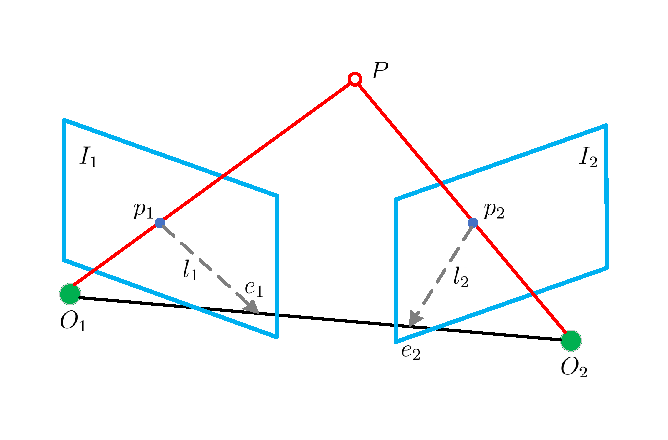
\includegraphics[width=0.25\textwidth, angle=-90]{figures/chapter3/fig3_8}
	\caption{对极几何约束示意图}\label{fig3_8}
\end{figure}

假设 $P$ 的3D空间坐标为 $\boldsymbol{P}=[X, Y, Z]^{T} $ ,根据2.1.1小节研究的针孔相机模型,可以得到 $P$ 与 $p_1,p_2 $ 的关系为:
\begin{equation}
\label{eqn:3.58}
\setlength{\abovedisplayskip}{6pt}
\setlength{\belowdisplayskip}{6pt}
\begin{aligned}
s_{1} \boldsymbol{p}_{1} &= \boldsymbol{K} \boldsymbol{P},  \\
s_{2} \boldsymbol{p}_{2} &= \boldsymbol{K}(\boldsymbol{R} \boldsymbol{P}+\boldsymbol{t})
\end{aligned}
\end{equation}
其中, $\bm{K} $ 为相机内参, $s_1,s_2 $ 为尺度因子。如果使用齐次坐标,式(\ref{eqn:3.58})可以写为:
\begin{equation}
\label{eqn:3.59}
\setlength{\abovedisplayskip}{6pt}
\setlength{\belowdisplayskip}{6pt}
\begin{aligned}
\boldsymbol{p}_{1} &= \boldsymbol{K} \boldsymbol{P},  \\
\boldsymbol{p}_{2} &= \boldsymbol{K}(\boldsymbol{R} \boldsymbol{P}+\boldsymbol{t})
\end{aligned}
\end{equation}
设 $p_1,p_2 $ 的归一化平面坐标为 $\boldsymbol{x}_{1}, \boldsymbol{x}_{2} $ ,易知:
\begin{equation}
\label{eqn:3.60}
\setlength{\abovedisplayskip}{6pt}
\setlength{\belowdisplayskip}{6pt}
\begin{aligned}
\boldsymbol{x}_{1} &=\boldsymbol{K}^{-1} \boldsymbol{p}_{1} \\
\boldsymbol{x}_{2} &=\boldsymbol{K}^{-1} \boldsymbol{p}_{2}
\end{aligned}
\end{equation}
联立式(\ref{eqn:3.59})和(\ref{eqn:3.60})可得:
\begin{equation}
\label{eqn:3.61}
\boldsymbol{x}_{2}=\boldsymbol{R} \boldsymbol{x}_{1}+\boldsymbol{t}
\end{equation}
等式(\ref{eqn:2.61})两边同时左乘 $\left[\bm{t}\right]_\times $ 可得:
\begin{equation}
\label{eqn:3.62}
\setlength{\abovedisplayskip}{6pt}
\setlength{\belowdisplayskip}{6pt}
\left[\boldsymbol{t}\right]_\times \boldsymbol{x}_{2}= \left[\boldsymbol{t}\right]_\times  \boldsymbol{R} \boldsymbol{x}_{1}
\end{equation}
等式(\ref{eqn:3.62})两边同时左乘 $\bm{x}_{2}^{T} $ 可得:
\begin{equation}
\label{eqn:3.63}
\setlength{\abovedisplayskip}{6pt}
\setlength{\belowdisplayskip}{6pt}
\boldsymbol{x}_{2}^{T} \left[\boldsymbol{t}\right]_\times \boldsymbol{x}_{2}=
\boldsymbol{x}_{2}^{T} \left[\boldsymbol{t}\right]_\times \boldsymbol{R} \boldsymbol{x}_{1}
\end{equation}
由于向量 $\left[\boldsymbol{t}\right]_\times \boldsymbol{x}_{2} $ 和 $\bm{x}_2 $ 垂直,所以等式(\ref{eqn:3.63})左侧等于0,所以:
\begin{equation}
\label{eqn:3.64}
\setlength{\abovedisplayskip}{6pt}
\setlength{\belowdisplayskip}{6pt}
\boldsymbol{x}_{2}^{T} \left[\boldsymbol{t}\right]_\times \boldsymbol{R} \boldsymbol{x}_{1} = 0
\end{equation}
联立公式(\ref{eqn:3.60})和(\ref{eqn:3.64})可得:
\begin{equation}
\label{eqn:3.65}
\setlength{\abovedisplayskip}{6pt}
\setlength{\belowdisplayskip}{6pt}
\boldsymbol{p}_{2}^{T} \boldsymbol{K}^{-T} \left[\boldsymbol{t}\right]_\times \boldsymbol{R} \boldsymbol{K}^{-1} \boldsymbol{p}_{1}=0
\end{equation}
公式(\ref{eqn:3.64})和(\ref{eqn:3.65})称为对极约束,其几何意义是 $O_{1}, P, O_{2} $ 三点共面。记
\begin{equation}
\label{eqn:3.66}
\setlength{\abovedisplayskip}{6pt}
\setlength{\belowdisplayskip}{6pt}
\begin{aligned}
\boldsymbol{E} &= \left[\boldsymbol{t}\right]_\times \boldsymbol{R} \\
\boldsymbol{F} &= \boldsymbol{K}^{-T} \left[\boldsymbol{t}\right]_\times \boldsymbol{R} \boldsymbol{K}^{-1} \\
&= \boldsymbol{K}^{-T} \boldsymbol{E} \boldsymbol{K}^{-1} 
\end{aligned}
\end{equation}
称 $\boldsymbol{F} $ 为基本矩阵,$\boldsymbol{E} $ 为本质矩阵。可见 $\boldsymbol{F} $ 和 $\boldsymbol{E} $ 之间只相差了一个相机内参 。这样以来,就可以根据匹配的关键点,通过对极约束求出 $\boldsymbol{F} $ 或者 $\boldsymbol{E} $ ,进而求出 $\boldsymbol{R}, \boldsymbol{t} $ 。

矩阵 $\left[\boldsymbol{t}\right]_\times \boldsymbol{R}  $ 有六个自由度,由对极约束(\ref{eqn:3.64})可知 $\bm{E} $ 具有尺度不确定性,所以 $\bm{E} $ 只有五个自由度。这表明,最少使用五对匹配的关键点就可以求出 $\bm{E} $ \upcite{nister2004efficient}。由于本质矩阵 $\bm{E} $ 的奇异值形式是 $[\sigma, \sigma, 0]^{T} $ \upcite{hartley2003multiple},这种非线性性质使得求解线性方程变得困难。因此,通常使用八对匹配的关键点来求解 $\bm{E} $ ,这种方法称为八点发(Eight-point-algorithm)\upcite{hartley2003multiple}\upcite{Hartley1997In}\upcite{longuet1981computer}。

假设有一对匹配好的关键点,其归一化的齐次坐标为:$\boldsymbol{x}_{1}=\left[u_{1}, v_{1}, 1\right]^{T}$ ,$\boldsymbol{x}_{2}=\left[u_{2}, v_{2}, 1\right]^{T}  $ 。由对极约束(3.64)可得,
\begin{equation}
\label{eqn:3.67}
\left(u_{1}, v_{1}, 1\right) \left( \begin{array}{ccc}{e_{1}} & {e_{2}} & {e_{3}} \\ {e_{4}} & {e_{5}} & {e_{6}} \\ {e_{7}} & {e_{8}} & {e_{9}}\end{array}\right) \left( \begin{array}{l}{u_{2}} \\ {v_{2}} \\ {1}\end{array}\right)=0
\end{equation}
中间的矩阵是本质矩阵 $\bm{E} $ 。改变 $\bm{E} $ 的形式,令 $ \boldsymbol e=\left[e_{1}, e_{2}, e_{3}, e_{4}, e_{5}, e_{6}, e_{7}, e_{8}, e_{9}\right]^{T} $ ,则式(\ref{eqn:3.67})可变形为:
\begin{equation}
\label{eqn:3.68}
\setlength{\abovedisplayskip}{6pt}
\setlength{\belowdisplayskip}{6pt}
\left[u_{1} u_{2}, u_{1} v_{2}, u_{1}, v_{1} u_{2}, v_{1} v_{2}, v_{1}, u_{2}, v_{2}, 1\right] \cdot \boldsymbol e=0
\end{equation}

对于其他七个点可以得到类似的方程,将这八个方程放在一起写成矩阵的形式,可得:
\begin{equation}
\label{eqn:3.69}
\left( \begin{array}{ccccccccc}
{u_{1}^{1} u_{2}^{1}} & {u_{1}^{1} v_{2}^{1}} & {u_{1}^{1}} & {v_{1}^{1} u_{2}^{1}} & {v_{1}^{1} v_{2}^{1}} & {v_{1}^{1}} & {u_{2}^{1}} & {v_{2}^{1}} & {1}  \\ 
{u_{1}^{2} u_{2}^{2}} & {u_{1}^{2} v_{2}^{2}} & {u_{1}^{2}} & {v_{1}^{2} u_{2}^{2}} & {v_{1}^{2} v_{2}^{2}} & {v_{1}^{2}} & {u_{2}^{2}} & {v_{2}^{2}} & {1} \\ 
{\vdots} & {\vdots} & {\vdots} & {\vdots} & {\vdots} & {\vdots} & {\vdots} & {\vdots} \\ 
{u_{1}^{8} u_{2}^{8}} & {u_{1}^{8} v_{2}^{8}} & {u_{1}^{8}} & {v_{1}^{8} u_{2}^{8}} & {v_{1}^{8} v_{2}^{8}} & {v_{1}^{8}} & {u_{2}^{8}} & {v_{2}^{8}} & {1}
\end{array}\right)
\left( \begin{array}{c}{e_{1}} \\ {e_{2}} \\ {e_{3}} \\ {e_{4}} \\ {e_{5}} \\ {e_{6}} \\ {e_{8}} \\ {e_{8}} \\ {e_{9}}\end{array}\right)
=0
\end{equation}

通过求解这个方程组就可以得到本质矩阵  $\bm{E} $ ,然后通过奇异值分解(SVD)来计算 $\boldsymbol{R}, \boldsymbol{t} $ 。假设  $\bm{E} $  的奇异值分解为:
\begin{equation}
\label{eqn:3.70}
\setlength{\abovedisplayskip}{6pt}
\setlength{\belowdisplayskip}{6pt}
\boldsymbol{E}= \boldsymbol{U} \boldsymbol{\Sigma} \boldsymbol{V}^{T}
\end{equation}
其中,$\boldsymbol{U},\boldsymbol{V} $ 是正交矩阵,$\boldsymbol{\Sigma} $ 是奇异值矩阵。由 $\bm{E} $ 的非线性性质可得 $\boldsymbol{\Sigma}=\operatorname{diag}(\sigma, \sigma, 0) $ 。在SVD分解过程中可以发现,一个本质矩阵对应两组可能的 $\boldsymbol{R}, \boldsymbol{t} $:
\begin{equation}
\label{eqn:3.71}
\begin{aligned}
\left[\boldsymbol{t}_{1}\right]_\times&= \boldsymbol{U} \boldsymbol{R}_{Z}\left(\frac{\pi}{2}\right) \boldsymbol{\Sigma} \boldsymbol{U}^{T}, \quad \boldsymbol{R}_{1}=\boldsymbol{U} \boldsymbol{R}_{Z}^{T}\left(\frac{\pi}{2}\right) \boldsymbol{V}^{T} \\
\left[\boldsymbol{t}_{2}\right]_\times &= \boldsymbol{U} \boldsymbol{R}_{Z}\left(-\frac{\pi}{2}\right) \boldsymbol{\Sigma} \boldsymbol{U}^{T}, \quad \boldsymbol{R}_{2}=\boldsymbol{U} \boldsymbol{R}_{Z}^{T}\left(-\frac{\pi}{2}\right) \boldsymbol{V}^{T} 
\end{aligned}
\end{equation}
其中,$\boldsymbol{R}_{Z}\left(\frac{\pi}{2}\right) $ 表示绕 轴旋转90°的旋转矩阵。$\bm{E} $ 的尺度不确定性导致 $\bm{E} $ 和 $-\bm{E} $ 是等价的,故对于 $-t$ 也会得到式(\ref{eqn:3.71})的结果。所以总共有四种可能的情况,如图\ref{fig3_9}所示。根据实际情况,分解出来的 $\boldsymbol{R}, \boldsymbol{t} $ 应该满足使得路标点的深度为正值,也就是说关键点对应的3D空间点 $P$ 应该和相机成像平面在同一侧,可见在图\ref{fig3_9}的4种情形中,只有第一种符合要求,从而确定该解为正确的解。
\begin{figure}[h]\setlength{\belowcaptionskip}{-12pt}
	\centering
	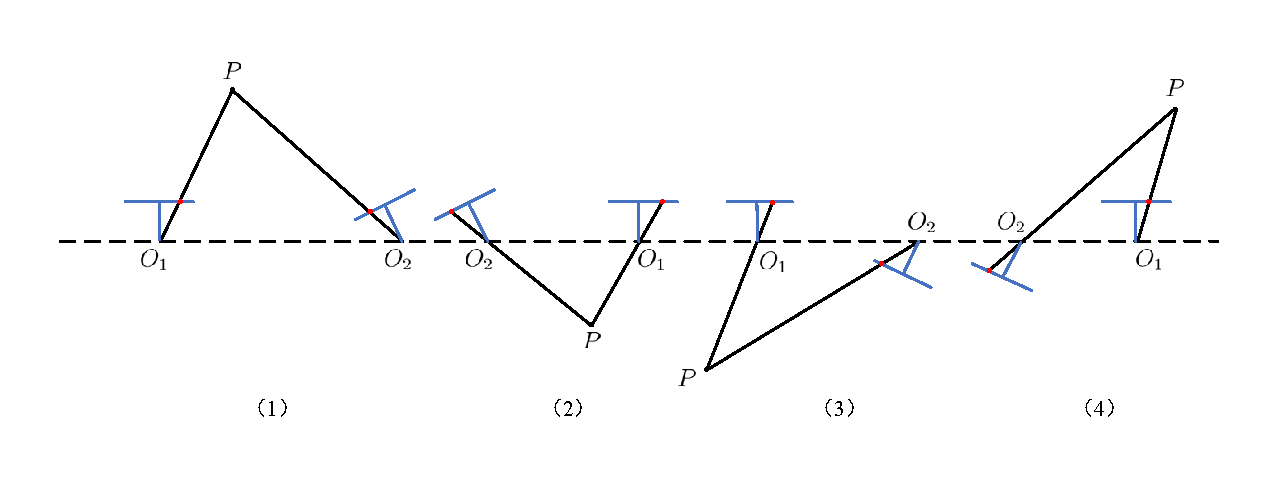
\includegraphics[width=0.3\textwidth, angle=-90]{figures/chapter3/fig3_9}
	\caption{分解本质矩阵得到的四种解}\label{fig3_9}
\end{figure}

2.三角化求路标点深度

在单目视觉SLAM中,无法直接获取路标点的深度信息,需要利用相机位姿通过三角测量(Triangulation,也称三角化)的方法来计算路标点深度。三角测量是指,在不同的方向观察目标点,通过两次观察的方向与目标点的夹角来确定目标的的距离。三角测量由高斯最先提出,在地理学和天文学中都有广泛的应用。与图\ref{fig3_8}类似,图\ref{fig3_10}展示了三角化计算路标点深度的示意图。
\begin{figure}[h]\setlength{\belowcaptionskip}{-12pt}
	\centering
	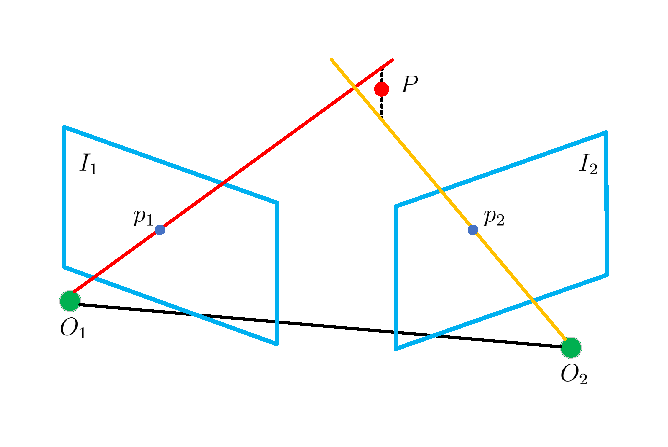
\includegraphics[width=0.25\textwidth, angle=-90]{figures/chapter3/fig3_10}
	\caption{三角化计算路标点深度}\label{fig3_10}
\end{figure}

以左边图像 $I_1 $ 为参考帧,假设右边图像  $I_2 $ 的旋转和平移为 $\boldsymbol{R}, \boldsymbol{t} $ 。理想情况下,射线 $O_1p_1 $ 和射线$O_2p_2 $ 会相交于点 $P$ ,点 $P$ 是 $p_1,p_2 $ 对应的三维空间坐标点。但是,实际情况下,由于传感器有噪声,射线 $O_1p_1 $ 和射线$O_2p_2 $通常不会严格的相交于点 $P$ ,甚至在三维空间中都不能相交。这种情况下通常利用最小二乘法来求解。

设 $\boldsymbol{x}_{1}, \boldsymbol{x}_{2} $ 是 $p_1,p_2 $ 的归一化坐标,由对极约束可得:
\begin{equation}
\label{eqn:3.72}
\setlength{\abovedisplayskip}{6pt}
\setlength{\belowdisplayskip}{6pt}
s_{1} \boldsymbol{x}_{1}=s_{2} \boldsymbol{R} \boldsymbol{x}_{2}+\boldsymbol{t}
\end{equation}
其中 $s_{1}, s_{2} $ 分别为 $p_1,p_2 $ 的深度。将等式(\ref{eqn:3.72})两边同时乘以 $\left[ \bm{x}_1 \right]_\times$ 得,
\begin{equation}
\label{eqn:3.73}
\setlength{\abovedisplayskip}{6pt}
\setlength{\belowdisplayskip}{6pt}
s_{1} \left[\boldsymbol{x}_{1}\right]_\times \boldsymbol{x}_{1}=0=s_{2} \left[\boldsymbol{x}_{1}\right]_\times \boldsymbol{R} \boldsymbol{x}_{2}+ \left[\boldsymbol{x}_{1}\right]_\times \boldsymbol{t}
\end{equation}

因为 $\boldsymbol{R}, \boldsymbol{t} $ 已知,故可以直接算出深度 $s_2 $ 。同理可得 $s_1 $ 。当然,根据刚才的分析,噪声的存在会使等式(3.73)不严格的等于0。所以需使用最小二乘法求解。

值得注意的是,由于本质矩阵 $\bm{E} $ 的尺度不确定性,计算出的路标点深度是没有尺度的,只有大小,也就是说此时得到的深度没有单位度量。在后面的联合初始化中,通过将视觉和IMU对齐来恢复出单目视觉的尺度信息。

三角测量是通过在不同的方向上观察路标点计算而得到的深度,因此相机必须要有平移,在纯旋转的情况下三角测量失效。在有平移的情况下,三角测量还存在一个矛盾的问题。这个矛盾是由像素的不确定性导致的。

如图\ref{fig3_11}所示,当相机的平移 $t$ 很小时,像素由于相机测量噪声产生的微小不确定性 $\delta \theta $,将导致计算的深度值有较大的不确定性$\delta d $ 。对比图\ref{fig3_11}的左右两图可以发现,当像素不确定性一样的情况下,较大的平移  $t$ 会产生更小的深度不确定性 $\delta d $ 。所以,在相机分辨率一样的情况下,较大的平移会使得三角测量更准确。
但是,并不是平移量越大越好,因为太大的平移量会图像特征跟踪(匹配)失败。因此就会产生一个三角化矛盾:增大平移会导致特征跟踪(匹配)失败,而减小平移又会降低三角测量的精度。
\begin{figure}[h]\setlength{\belowcaptionskip}{-12pt}
	\centering
	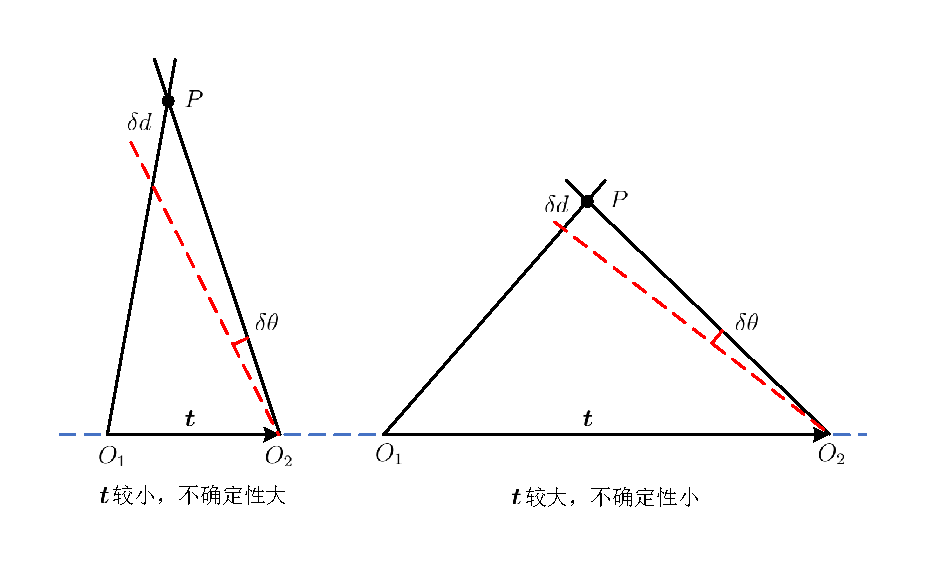
\includegraphics[width=0.35\textwidth, angle=-90]{figures/chapter3/fig3_11}
	\caption{三角测量的矛盾}\label{fig3_11}
\end{figure}

3.PnP求位姿

通过对极约束和三角测量已经可以计算出相机的姿态以及路标点的3D空间位置(没有尺度信息),那么能否根据已经计算出来的3D路标点,以及该路标点在其他图像帧中的2D投影坐标,来计算其他图像帧对应的相机姿态呢?当然可以,PnP正是求解此问题的方法,也就是说,当知道$n$个3D空间点以及他们在图像中的投影位置时,可以用PnP来求解相机的位姿。

求解PnP有很多种方法,比如使用3对点的P3P\upcite{gao2003complete},直接线性变换(Direct Linear Transform,DLT),EPnP(Efficient PnP)\upcite{lepetit2009epnp},UPnP\upcite{penate2013exhaustive}等等。下面研究DLT方法。

假设3D空间中的一点 $P$ ,用齐次坐标表示为 $\boldsymbol{P}=(X, Y, Z, 1)^{T} $ ,其在某一副图像中的投影点为 $\boldsymbol{x}_{1}$ ,用齐次坐标表示其在归一化平面上的坐标 $\boldsymbol{x}_{1}=\left(u_{1}, v_{1}, 1\right)^{T} $ 。该图像对应的相机位姿为 $\boldsymbol{R}, \boldsymbol{t} $ ,将 $\boldsymbol{R}, \boldsymbol{t} $ 放在一起构成一个增广矩阵 $\boldsymbol{T}= [ \boldsymbol{R} | \boldsymbol{t}] $ , $ \boldsymbol{T} $ 为3×4矩阵。根据3D空间点和归一化平面坐标点之间的映射关系可得,
\begin{equation}
\label{eqn:3.74}
s \left( \begin{array}{c}{u_{1}} \\ {v_{1}} \\ {1}\end{array}\right)=\left( \begin{array}{cccc}{t_{1}} & {t_{2}} & {t_{3}} & {t_{4}} \\ {t_{5}} & {t_{6}} & {t_{7}} & {t_{8}} \\ {t_{9}} & {t_{10}} & {t_{11}} & {t_{12}}\end{array}\right) \left( \begin{array}{c}{X} \\ {Y} \\ {Z} \\ {1}\end{array}\right)
\end{equation}
其中,中间得矩阵为 $ \boldsymbol{T} $ 的展开式。可以利用最后一行等式将式(\ref{eqn:3.74})中的尺度 $s$ 消去,得到两个约束等式:
\begin{equation}
\label{eqn:3.75}
\begin{aligned}
u_{1} &= \frac{t_{1} X+t_{2} Y+t_{3} Z+t_{4}}{t_{9} X+t_{10} Y+t_{11} Z+t_{12}} \\
v_{1} &= \frac{t_{5} X+t_{6} Y+t_{7} Z+t_{8}}{t_{9} X+t_{10} Y+t_{11} Z+t_{12}}
\end{aligned}
\end{equation}
令 $ \boldsymbol{T} $ 的行向量为:
\begin{equation}
\label{eqn:3.76}
\begin{aligned}
\boldsymbol{t} _{1} &= \left(t_{1}, t_{2}, t_{3}, t_{4}\right)^{T} \\
\boldsymbol{t} _{2} &= \left(t_{5}, t_{6}, t_{7}, t_{8}\right)^{T} \\
\boldsymbol{t} _{3} &= \left(t_{9}, t_{10}, t_{11}, t_{12}\right)^{T}
\end{aligned}
\end{equation}
则式(\ref{eqn:3.75})可以写为:
\begin{equation}
\label{eqn:3.77}
\begin{aligned}
\boldsymbol{t}_{1}^{T} \boldsymbol{P}-\boldsymbol{t}_{3}^{T} \boldsymbol{P} u_{1}=0 \\
\boldsymbol{t}_{2}^{T} \boldsymbol{P}-\boldsymbol{t}_{3}^{T} \boldsymbol{P} v_{1}=0
\end{aligned}
\end{equation}

可以观察到,一对3D路标点和2D关键点可以提供两个关于关于 $t$ 的线性约束项等式。那么 $N$ 对3D路标点和2D关键点可以提供 $2N$ 个约束项,写成矩阵形式为:
\begin{equation}
\label{eqn:3.78}
\left( \begin{array}{ccc}{\boldsymbol{P}_{1}^{T}} & {0} & {-u_{1} \boldsymbol{P}_{1}^{T}} \\ {0} & {\boldsymbol{P}_{1}^{T}} & {-v_{1} \boldsymbol{P}_{1}^{T}} \\ {\vdots} & {\vdots} & {\vdots} \\ {\boldsymbol{P}_{N}^{T}} & {0} & {-u_{N} \boldsymbol{P}_{N}^{T}} \\ {0} & {\boldsymbol{P}_{N}^{T}} & {-v_{N} \boldsymbol{P}_{N}^{T}}\end{array}\right) 
\left( \begin{array}{l}{\boldsymbol{t}_{1}} \\ {\boldsymbol{t}_{2}} \\ {\boldsymbol{t}_{3}}\end{array}\right)=0
\end{equation}
 $t$ 的维数为12,因此最少可以通过6对3D路标点和2D关键点就可以求解出矩阵 $ \boldsymbol{T} $ 。当匹配或跟踪的点对大于6对时,可以使用SVD方法求解。
 
 4.Bundle Adjustment
 
 BA(Bundle Adjustment)中文可译为“捆集调整”\upcite{triggs1999bundle}\upcite{granshaw1980bundle}。通过最小化重投影误差(Reprojection Error)来迭代优化求解问题。对于单目相机来说,使用PnP需要先求相机位姿,在求3D路标点位置,而BA将相机位姿和路标点位置看作优化变量,放在一起进行迭代优化。通常情况下,用BA来优化PnP估计的结果。
 
 假设有 $n$ 个3D空间点 $P$ ,在某一副图像中对应的投影坐标点为 $p$ ,第 $i$ 个3D空间点的坐标为 $\bm{P}_{i}=\left[X_{i}, Y_{i}, Z_{i}\right]^{T} $ ,对应的投影像素坐标为 $\boldsymbol{u}_{i}=\left[u_{i}, v_{i}\right]^{T} $。该图像对应的相机位姿为 $\bm{R}, \bm{t} $ ,其李代数为 $ \exp \left( \left[ \boldsymbol{\xi} \right]_\times \right) $ 。根据针孔相机模型可得:
\begin{equation}
\label{eqn:3.79}
\begin{aligned}
s_{i} \boldsymbol{u}_{i} &= \boldsymbol{K} \exp \left(  \left[\boldsymbol{\xi}\right]_\times  \right) \boldsymbol{P}_{i} \\
s_{i} \left[ \begin{array}{c}{u_{i}} \\ {v_{i}} \\ {1}\end{array}\right] &= \boldsymbol{K} \exp \left(  \left[\boldsymbol{\xi}\right]_\times \right) \left[ \begin{array}{c}{X_{i}} \\ {Y_{i}} \\ {Z_{i}} \\ {1}\end{array}\right]
\end{aligned}
\end{equation}
其中,$s_i $ 是尺度,$\bm{K} $ 是相机内参。然而,实际情况中相机是有噪声的,噪声使得等式(\ref{eqn:3.79})不相等,有一个误差。将每个观测点噪声带来的误差相加构成一个代价函数,建模为最小二乘问题,通过最小化代价函数来寻找最优的 $\bm{P}_i$ 和 $ \left[\boldsymbol{\xi}\right]_\times  $ :
\begin{equation}
\label{eqn:3.80}
\boldsymbol{e} =\arg \min _{\boldsymbol{\xi}} \frac{1}{2} \sum_{i=1}^{n}\left\|\boldsymbol{u}_{i}-\frac{1}{s_{i}} \boldsymbol{K} \exp \left(  \left[\boldsymbol{\xi}\right]_\times  \right) \boldsymbol{P}_{i}\right\|_{2}^{2}
\end{equation}

对于最小二乘问题,通常使用高斯-牛顿法或者LM方法求解。在使用G-N或者L-M方法的时候,需要知道代价函数关于误差项的导数,也就是雅可比矩阵,这里不再详细推导,直接给出代价函数 $\boldsymbol{e} $ 关于相机位姿 $\boldsymbol{\xi} $ 和3D空间点 $P$ 的的雅可比矩阵:
\begin{equation}
\label{eqn:3.81}
\frac{\partial \bm{e}}{\partial \delta \bm{\xi}} = 
-\left[ \begin{array}{cccccc}
{\frac{f_{x}}{Z^{\prime}}} & {0} & {-\frac{f_{x} X^{\prime}}{Z^{\prime 2}}} &
{-\frac{f_{x} X^{\prime} Y^{\prime}}{Z^{\prime 2}}} & {f_{x}+\frac{f_{x} X^{2}}{Z^{\prime 2}}} & {-\frac{f_{x} Y^{\prime}}{Z^{\prime}}}  \\ 
{0} & {\frac{f_{y}}{Z^{\prime}}} & {-\frac{f_{y} Y^{\prime}}{Z^{\prime 2}}} &
{-f_{y}-\frac{f_{y} Y^{\prime 2}}{Z^{\prime 2}}} & {\frac{f_{y} X^{\prime} Y^{\prime}}{Z^{\prime 2}}} & {\frac{f_{y} X^{\prime}}{Z^{\prime}}} 
\end{array}\right]
\end{equation}
\begin{equation}
\label{eqn:3.82}
\frac{\partial \bm{e}}{\partial \boldsymbol{P}}=-\left[ \begin{array}{ccc}{\frac{f_{x}}{Z^{\prime}}} & {0} & {-\frac{f_{x} X^{\prime}}{Z^{\prime 2}}} \\ {0} & {\frac{f_{y}}{Z^{\prime}}} & {-\frac{f_{y} Y^{\prime}}{Z^{\prime 2}}}\end{array}\right] \boldsymbol{R}
\end{equation}
\subsection{纯视觉初始化}
为了减少计算量,初始化在一个滑动窗口内进行。首先检查窗口内当前的图像帧与其他帧的关键点对应关系,找到与当前帧匹配关键点数量最多的关键帧作为参考帧。然后使用对极几何求解基础矩阵,从而计算出当前帧与参考帧帧之间的变换矩阵。然后用SFM(Structure-From-Motion)\upcite{ullman1979interpretation}计算处滑窗内的所有关键帧的位姿以及路标点的3D空间坐标,SFM具体步骤包括:

(1)通过三角化得到当前帧和参考帧的路标点;

(2)对于当前帧和参考帧之间的所有帧用PnP算法求解其位姿;

(3)通过三角化得到当前帧和参考帧之间的所有帧的路标点;

(4)对于当前帧和第一帧之间的所有帧用PnP算法求解其位姿;

(5)通过三角化得到当前帧和第一帧之间的所有帧的路标点;

(6)对于其他没有被三角化的关键点,对其三角化得到剩余的路标点;

(7)通过BA对滑动窗口内的所有关键帧位姿进行优化。

在完成了SFM后,已经可以估计出滑动窗口内所有关键帧的位姿,然而,视觉初始化可能不是一次就能成功,这个时候,关键帧的总数可能会超过窗口大小,还需要再次使用PnP算法估计出那些不被包括在窗口内的关键帧的位姿。

至此,纯视觉初始化就完成了。值得注意的是,在纯视觉初始化的时候,将第一帧图像$ {(\cdot)}^{c_0} $ 作为参考帧,因此需要将位姿从第一帧图像坐标系转换到IMU坐标系,方法如下:
\begin{equation}
\label{eqn:3.83}
\begin{split}
\mathbf{q}_{b_k}^{c_0}&=\mathbf{q}_{c_k}^{c_0}\otimes(\mathbf{q_c^b})^{-1} \\
s\bar{\mathbf{p}}_{b_k}^{c_0}&=s\bar{\mathbf{p}}_{c_k}^{c_0}-\mathbf{R}_{b_k}^{c_0}\mathbf{p}_c^b,
\end{split}
\end{equation}
其中,$ \mathbf{p}_c^b,\mathbf{q}_c^b $ 是外参(Visual到IMU)。
\subsection{视觉/惯性联合初始化}
如图\ref{fig3_12}所示,视觉/惯性联合初始化是将IMU预积分的值和出视觉初始化的值进行对齐,从而计算出绝对尺度 $s $ 、陀螺仪bias、重力矢量 $\mathbf{g} $ 和速度 $\mathbf{v}$ 。注意,不计算加速度计的bias,因为重力加速度的值要远远大于加速度计的bias,这导致加速度计的bias很难被观测到\upcite{mur2017visual},因此忽略加速度计bias的影响,只计算陀螺仪的bias。
\begin{figure}[h]\setlength{\belowcaptionskip}{-12pt}
	\centering
	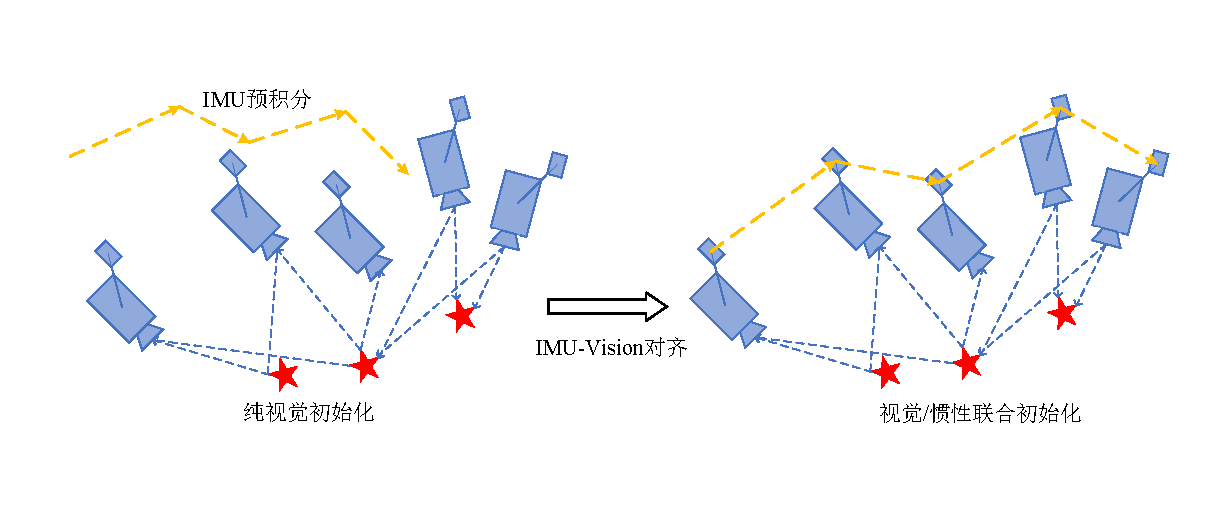
\includegraphics[width=0.3\textwidth, angle=-90]{figures/chapter3/fig3_12}
	\caption{视觉/惯性联合初始化示意图}\label{fig3_12}
\end{figure}

(1)矫正陀螺仪bias

考虑滑动窗口内连续两帧图像 $ b_k $ 和 $b_{k+1}$ ,从纯视觉初始化中得到的两帧之间的旋转 $ {\mathbf{q}_{b_{k+1}}^{c_0}}^{-1} \mathbf{q}_{b_k}^{c_0} $  应该和IMU预积分得到旋转 $ \bm{\gamma}_{b_{k+1}}^{b_k} $ 相等。通过式(3.18) 线性化IMU预积分项,并定义代价函数:
\begin{equation}
\label{eqn:3.84}
\underset{\delta b_w}{\text{min}}\sum_{k\in \mathcal{B} }\left\|{\mathbf{q}_{b_{k+1}}^{c_0}}^{-1}\otimes\mathbf{q}_{b_k}^{c_0}\otimes\bm{\gamma}_{b_{k+1}}^{b_k}\right\|^2 
\end{equation}
其中,$\mathcal{B} $ 代表窗口中的所有帧,
\begin{equation}
\label{eqn:3.85}
\bm{\gamma}_{b_{k+1}}^{b_k}\approx\hat{\bm{\gamma}}_{b_{k+1}}^{b_k}\otimes\begin{bmatrix}
1 \\ \frac{1}{2}\mathbf{J}_{b_w}^\gamma\delta\mathbf{b}_w
\end{bmatrix}
\end{equation}
代价函数(\ref{eqn:3.84})的最小值为单位四元数,所以可以将式(\ref{eqn:3.84})写为:
\begin{equation}
\label{eqn:3.86}
{ \mathbf{ q}_{b_{k+1}}^{c_{0}}}^{-1} \otimes \mathbf{q}_{b_{k}}^{c_{0}} \otimes \bm{\gamma}_{b_{k+1}}^{b_{k}}=\left[ \begin{array}{l}{\mathbf{1}} \\ {0}\end{array}\right]
\end{equation}
将式(\ref{eqn:3.85})代入式(\ref{eqn:3.86})得,
\begin{equation}
\label{eqn:3.87}
\begin{aligned}
\hat{\bm{\gamma}}_{b_{k+1}}^{b_{k}} \otimes\left[\frac{1}{2} \mathbf{J}_{b_{\omega}}^{\gamma} \delta \mathbf{b}_{\omega}\right]
&= \mathbf{q}_{b_{k}}^{c_{0}-1} \otimes \mathbf{q}_{b_{k+1}}^{c_{0}} \otimes \left[ \begin{array}{l}{\mathbf{1}} \\ {0}\end{array}\right] \\
\Longrightarrow \quad \quad \left[\frac{1}{2} \mathbf{J}_{b_{\omega}}^{\gamma} \delta \mathbf{b}_{\omega}\right]
&= \hat{\bm{\gamma}}_{b_{k+1}}^{b_{k}-1} \otimes \mathbf{q}_{b_{k}}^{c_{0}-1} \otimes \mathbf{q}_{b_{k+1}}^{c_{0}} \otimes \left[ \begin{array}{l}{\mathbf{1}} \\ {0}\end{array}\right] \\
\Longrightarrow \quad \quad \quad \quad  \mathbf{J}_{b_{\omega}}^{\gamma} \delta \mathbf{ b}_{\omega} 
&=2 \mathbf{Im}\left( (\hat{\bm{\gamma}}^{b_{k}}_{b_{k+1}})^{-1} \otimes \mathbf{q}_{b_{k}}^{c_{0}-1} \otimes \mathbf{q}_{b_{k+1}}^{c_{0}}\right)
\end{aligned}
\end{equation}
其中 $\mathbf{Im} $ 表示虚部。将式(3.87)两边同时乘以 ${\mathbf{J}_{b_{\omega}}^{\gamma}}^{T}$ ,使等式左边变为正定矩阵,
\begin{equation}
\label{eqn:3.88}
{\mathbf{J}_{b_{\omega}}^{\gamma}}^{T}
\mathbf{J}_{b_{\omega}}^{\gamma} \delta \mathbf{b}_{\omega} = 
2 {\mathbf{J}_{b_{\omega}}^{\gamma}}^{T} \mathbf{Im}\left( (\hat{\bm{\gamma}}_{b_{k+1}}^{b_{k}})^{-1} \otimes \mathbf{q}_{b_{k}}^{c_{0}-1} \otimes \mathbf{q}_{b_{k+1}}^{c_{0}}\right)
\end{equation}

这样就可以直接通过Cholesky分解法得到陀螺仪的bias。然后再用计算出的陀螺仪bias再次重新积分IMU。

(2)速度、重力矢量和尺度因子初始化

将速度、重力和尺度因子放在一起作为优化变量,
\begin{equation}
\label{eqn:3.89}
\setlength{\abovedisplayskip}{6pt}
\setlength{\belowdisplayskip}{6pt}
\mathcal{X}_I=[\mathbf{v}_{b_0}^{b_0},\mathbf{v}_{b_1}^{b_1},\cdots\mathbf{v}_{b_n}^{b_n},\mathbf{g}^{c_0},s]
\end{equation}
其中,当取第 $k$ 帧图像时,$\mathbf{v}_{b_k}^{b_k} $ 是IMU坐标系下的速度,$ \mathbf{g}^{c_0} $ 是第0帧图像对应得相机坐标系下的重力向量,$s $ 是尺度因子。

考虑窗口中连续的两帧图像 $b_{k} $ 和 $b_{k+1} $ ,那么式(\ref{eqn:3.16})可以写成:
\begin{equation}
\label{eqn:3.90}
\begin{split}
\bm{\alpha}_{b_{k+1}}^{b_k}&=  
\mathbf{R}_{c_0}^{b_k}(s(\bar{\mathbf{p}}_{b_{k+1}}^{c_0}-\bar{\mathbf{p}}_{b_k}^{c_0})+\frac{1}{2}\mathbf{g}^{c0}\Delta t_k^2-\mathbf{R}_{b_k}^{c_0}\mathbf{v}_{b_k}^{b_k}\Delta t_k) \\
\bm{\beta}_{b_{k+1}}^{b_k}&=
\mathbf{R}_{c_0}^{b_k}(\mathbf{R}_{b_{k+1}}^{c_0}\mathbf{v}_{b_{k+1}}^{b_{k+1}}+\mathbf{g}^{c0}\Delta t_k-\mathbf{R}_{b_k}^{c_0}\mathbf{v}_{b_k}^{b_k}).
\end{split}
\end{equation}

定义残差项为  $b_{k} $ 和 $b_{k+1} $ 帧图像间的IMU预积分量 $\hat{\bm{\alpha}}_{b_{k+1}}^{b_k},\hat{\bm{\beta}}_{b_{k+1}}^{b_k} $与预测值 $\bm{\alpha}_{b_{k+1}}^{b_k},\bm{\beta}_{b_{k+1}}^{b_k} $之间的误差,
\begin{equation}
\label{eqn:3.91}
\begin{aligned}
\mathbf{r}\left(\hat{\mathbf{Z}}_{b_{k+1}}^{b_{k}}, \mathcal{X}_{I}\right)
&= 
\left[ \begin{array}{c}
{\delta \bm{\alpha}_{b_{k+1}}^{b_{k}}} \\ {\delta \bm{\beta}_{b_{k+1}}^{b_{k}}}
\end{array}\right]  \\ 
&=
\left[ \begin{array}{c}
\hat{\bm{\alpha}}_{b_{k+1}}^{b_{k}}  -  
	\mathbf{R}_{c_0}^{b_k}(s(\bar{\mathbf{p}}_{b_{k+1}}^{c_0}-\bar{\mathbf{p}}_{b_k}^{c_0})+\frac{1}{2}\mathbf{g}^{c0}\Delta t_k^2-\mathbf{R}_{b_k}^{c_0}\mathbf{v}_{b_k}^{b_k}\Delta t_k) \\ 
	\hat{\bm{\beta}}_{b_{k+1}}^{b_{k}}-
		\mathbf{R}_{c_0}^{b_k}(\mathbf{R}_{b_{k+1}}^{c_0}\mathbf{v}_{b_{k+1}}^{b_{k+1}}+\mathbf{g}^{c0}\Delta t_k-\mathbf{R}_{b_k}^{c_0}\mathbf{v}_{b_k}^{b_k})
		\end{array}\right]
		\end{aligned}
\end{equation}
将式(\ref{eqn:3.83})代入式(\ref{eqn:3.91})中的$\delta \hat{\bm{\alpha}}_{b_{k+1}}^{b_{k}} $并写成 $\mathbf{H} \mathbf{x}=\mathbf{b} $ 的形式,
\begin{equation}
\label{eqn:3.92}
\mathbf{ R}_{c_{0}}^{b_{k}}(\overline{\mathbf{ p}}_{c_{k+1}}^{c_{0}}-\overline{\mathbf{ p}}_{c_{k}}^{c_{0}})_{S}-\Delta t_{k} \mathbf{ v}_{b_{k}}^{b_{k}}
+\frac{1}{2} \mathbf{ R}_{c_{0}}^{b_{k}} \Delta t_{k}^{2} \mathbf{ g}^{c_{0}}
=\bm{\alpha}_{b_{k+1}}^{b_{k}}-\mathbf{ p}_{c}^{b_{k}} + \mathbf{R}_{c_0}^{b_k}\mathbf{ R}_{b_{k+1}}^{c_{0}} \mathbf{ p}_{c}^{b}
\end{equation}
写成矩阵形式,
\begin{equation}
\label{eqn:3.93}
\begin{aligned}
& \left[\begin{array}{cccc}
- \mathbf{I} \Delta t_{k} & 0 & \frac{1}{2} \mathbf{R}_{c_{0}}^{b_{k}} \Delta t_{k}^{2} & \mathbf{R}_{c_{0}}^{b_{k}}(\overline{\mathbf{p}}_{c_{k+1}}^{c_{0}}-\overline{\mathbf{p}}_{c_{k}}^{c_{0}}) \\
\end{array}\right]
\left[ \begin{array}{c}{\mathbf{v}_{b_{k}}^{b_{k}}} \\ {\mathbf{v}_{b_{k+1}}^{b_{k+1}}} \\ {\mathbf{g}^{c_{0}}} \\ {S} \end{array}\right] \\
&=
\bm{\alpha}_{b_{k+1}}^{b_{k}}-\mathbf{p}_{c_{0}}^{b_{k}} + \mathbf{R}_{c_0}^{b_k}\mathbf{R}_{b_{k+1}}^{c_{0}} \mathbf{p}_{c}^{b}
\end{aligned}
\end{equation}
同理,将 $\delta \hat{\bm{\beta}}_{b_{k+1}}^{b_{k}} $ 也可以写成类似式(\ref{eqn:3.93})的形式,并与式(\ref{eqn:3.93})合并写成如下矩阵形式:
\begin{equation}
\label{eqn:3.94}
\begin{aligned}
& \left[ \begin{array}{cccc}
- \mathbf{I} \Delta t_{k} & 0 & \frac{1}{2} \mathbf{R}_{c_{0}}^{b_{k}} \Delta t_{k}^{2} & \mathbf{R}_{c_{0}}^{b_{k}}(\overline{\mathbf{p}}_{c_{k+1}}^{c_{0}}-\overline{\mathbf{p}}_{c_{k}}^{c_{0}}) \\
{- \mathbf{ I}} & {\mathbf{R}_{c_{0}}^{b_{k}} \mathbf{R}_{b_{k+1}}^{c_{0}}} & {\mathbf{R}_{c_{0}}^{b_{k}} \Delta t_{k}} & {0}
\end{array}\right] 
\left[ \begin{array}{c}
{\mathbf{v}_{b_{k}}^{b_{k}}} \\ {\mathbf{v}_{b_{k+1}}^{b_{k+1}}} \\ {\mathbf{g}^{c_{0}}} \\ s
\end{array}\right] \\
&=\left[ \begin{array}{c}
\bm{\alpha}_{b_{k+1}}^{b_{k}}-\mathbf{p}_{c_{0}}^{b_{k}} + \mathbf{R}^{b_k}_{c_0}\mathbf{R}_{b_{k+1}}^{c_{0}} \mathbf{p}_{c}^{b} \\
{\bm{\beta}_{b_{k+1}}^{b_{k}}}
\end{array}\right]
\end{aligned}
\end{equation}
式(\ref{eqn:3.94})通过Cholesky分解可以解出 $\mathcal{X}_I $ 。

(3)重力矢量修正

由于噪声等原因,在上一步求出来的重力 $\mathbf{g}^{c_0} $ 是有误差的。通常情况下,重力大小是已知的,$g \approx 9.81 \mathrm{m} / \mathrm{s}^{2} $ 。因此,可以根据这个先验信息来修正上一步估计出来的 $\mathbf{g}^{c_0} $ 。
\begin{figure}[h]\setlength{\belowcaptionskip}{-12pt}
	\centering
	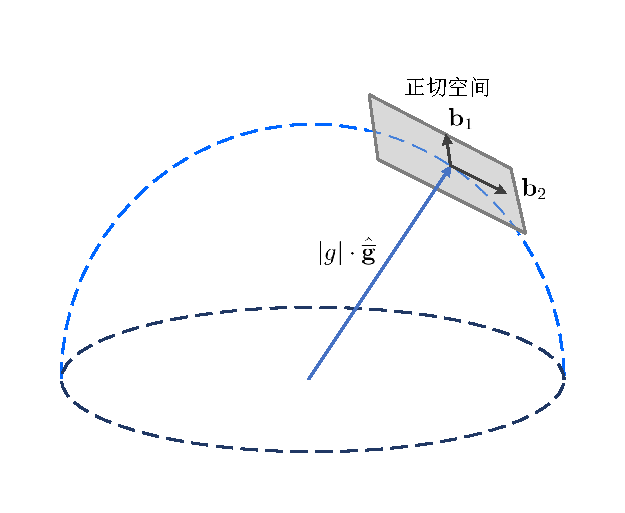
\includegraphics[width=0.25\textwidth, angle=-90]{figures/chapter3/fig3_13}
	\caption{两自由度重力矢量参数化示意图}\label{fig3_13}
\end{figure}

因为重力的大小已知,所以重力的自由度由3个变为2个。如图\ref{fig3_13},对重力重新参数化为:
\begin{equation}
\label{eqn:3.95}
\hat{\mathbf{g}} = g \cdot \overline{\hat{\mathbf{g}}} +w_{1} \mathbf{b}_{1}+w_{2} \mathbf{b}_{2}
\end{equation}
其中,$\overline{\hat{\mathbf{g}}} $ 为上一步估计出来的重力的方向向量,$\mathbf{b}_1, \mathbf{b}_2 $ 是垂直于 $\overline{\hat{\mathbf{g}}} $ 的两个正交基。

将式(3.95)代入式(3.94)可得,
\begin{equation}
\label{eqn:3.96}
\begin{aligned}
& \left[ \begin{array}{cccc}
- \mathbf{I} \Delta t_{k} & 0 & \frac{1}{2} \mathbf{R}_{c_{0}}^{b_{k}} \Delta t_{k}^{2} \mathbf{b} & \mathbf{R}_{c_{0}}^{b_{k}}(\overline{\mathbf{p}}_{c_{k+1}}^{c_{0}}-\overline{\mathbf{p}}_{c_{k}}^{c_{0}}) \\
{- \mathbf{ I}} & {\mathbf{R}_{c_{0}}^{b_{k}} \mathbf{R}_{b_{k+1}}^{c_{0}}} & {\mathbf{R}_{c_{0}}^{b_{k}} \Delta t_{k}} \mathbf{b}  & {0}
\end{array}\right] 
\left[ \begin{array}{c}
{\mathbf{v}_{b_{k}}^{b_{k}}} \\ {\mathbf{v}_{b_{k+1}}^{b_{k+1}}} \\ \bm{\omega} \\s
\end{array}\right] \\
&=\left[ \begin{array}{c}
\bm{\alpha}_{b_{k+1}}^{b_{k}}-\mathbf{p}_{c_{0}}^{b_{k}} + \mathbf{R}^{b_k}_{c_0}\mathbf{R}_{b_{k+1}}^{c_{0}} \mathbf{p}_{c}^{b} -\frac{1}{2} \mathbf{R}_{c_{0}}^{b_{k}} \Delta t_{k}^{2} g \cdot \overline{\hat{\mathrm{g}}} \\
{\bm{\beta}_{b_{k+1}}^{b_{k}}} - \mathbf{R}_{c_{0}}^{b_{k}} \Delta t_{k} g\cdot \overline{\hat{\mathrm{g}}} 
\end{array}\right]
\end{aligned}
\end{equation}
其中,$\bm{\omega} =\left[\omega_{1}, \omega_{2}\right]^{T} $ ,$\mathbf{b} =\left[b_{1}, b_{2}\right]^{T} $ 。通过求解式(\ref{eqn:3.96}),可以得到 $\bm{\omega} $ ,从而可以得到修正后的 $\mathbf{g}^{c_{0}} $。通过 $\mathbf{g}^{c_{0}} $ 和世界坐标系的 $Z$ 轴方向,可以得到第一帧图像坐标系到世界坐标系的旋转 $\mathbf{q}_{C_{0}}^{w} $ ,从而可以将所有的状态变量变换到世界坐标系下。至此,初始化完成。

(4)初始航向修正

在联合初始化完成之后,使用磁力计测量的航向角对初始化过程中估计出的每一个关键帧的航向角进行修正,从而得到无偏的初始航向。
\section{本章小结}
本章对系统的前端和初始化算法进行了详细的阐述。其中,前端部分详细研究了特征的提取、跟踪和异常点剔除算法,并对IMU预积分理论的相关公式进行了详细的推导。系统初始化部分详细研究了visual初始化算法,以及Visual-IMU对齐方法。系统的前端和初始化在整个系统中占了很大的比重,前端和初始化的好坏影响后端非线性优化的精度,从而影响整个系统的定位精度。因此,一个良好的前端和初始化是实现系统高精度定位的基础。
\chapter{后端优化及闭环检测}
\label{chap:4}
在初始化完成后,采用基于滑动窗口的紧耦合单目VIO进行高精度和鲁棒性的状态估计。后端非线性优化是实现视觉/惯性紧耦合的关键步骤,闭环检测能够实现系统的重定位,提高系统的鲁棒性。本章将对后端非线性优化算法、闭环检测算法以及闭环优化算法进行详细分析与研究。
\section{后端非线性优化}
\subsection{状态向量和目标函数}
滑动窗口中的所有状态向量定义为:
\begin{equation}
\label{eqn:4.1}{\tiny }
\begin{split}
\mathcal{X}&=[\mathbf{x}_0,\mathbf{x}_1,\cdots\mathbf{x}_n,\mathbf{x}_c^b,\lambda_0,\lambda_1,\cdots\lambda_m] \\
\mathbf{x}_k&=[\mathbf{p}_{b_k}^w,\mathbf{v}_{b_k}^w,\mathbf{q}_{b_k}^w,\mathbf{b}_a,\mathbf{b}_g],k\in[0,n] \\
\mathbf{x}_c^b&=[\mathbf{p}_c^b,\mathbf{q}_c^b],
\end{split}
\end{equation}
其中 $\mathbf{x}_k $ 是第 $k$ 帧图像关联的IMU状态,它包含了IMU在世界坐标系中的位置、速度和方向,以及在IMU坐标系中的加速度计bias和陀螺仪bias, $n$ 是关键帧的总数,$m$ 是滑动窗口中的路标点总数,$\lambda_l$ 是第一次观测到的第 $l$ 个路标的逆深度(深度的倒数)。$\mathbf{x}_c^b $ 是外参。

定义目标函数为所有先验项和测量残差的马氏范数(Mahalanobis Norm)之和,从而得到最大后验概率估计:
\begin{equation}
\label{eqn:4.2}
\begin{split}
\underset{\mathcal{X}}{\text{min}}
\left\{
\left\| 
\mathbf{r}_p-\mathbf{H}_p\mathcal{X} 
\right\|^2+
\sum_{k\in\mathcal{B}}
\left\| 
\mathbf{r}_\mathcal{B}(\hat{\mathbf{z}}_{b_{k+1}}^{b_k},\mathcal{X}) 
\right\|
_{\mathbf{p}_{b_{k+1}}^{b_k}}^2+ \right. 
\left.\sum_{(l,j)\in\mathcal{C}}\rho(
\left\| 
\mathbf{r}_\mathcal{C}(\hat{\mathbf{z}}_l^{c_j},\mathcal{X}) 
\right\|
_{\mathbf{p}_l^{c_j}}^2) 
\right\}
\end{split}
\end{equation}
其中,$\mathbf{r}_\mathcal{B}(\hat{\mathbf{z}}_{b_{k+1}}^{b_k},\mathcal{X})  $ 和 $\mathbf{r}_\mathcal{C}(\hat{\mathbf{z}}_l^{c_j},\mathcal{X})  $ 分别是IMU和视觉测量的残差。$\mathcal{B} $ 是所有IMU测量的集合,$\mathcal{C} $ 是在当前滑动窗口中至少观察到两次的一组特征。$\left\{ \mathbf{r}_p,\mathbf{H}_p\right\} $ 是来自边缘化的先验信息。$\rho (\cdot) $ 为:
\begin{equation}
\label{eqn:4.3}
\rho(s)=
\left\{\begin{array}{lc}
s & s\leq 1,\\
2\sqrt{s}-1 & s\textgreater 1.
\end{array}\right. 
\end{equation}
将 $\left\| \mathbf{r}_\mathcal{C} \right\|^2 $ 代入式(\ref{eqn:4.3})得,
\begin{equation}
\label{eqn:4.4}
\frac{1}{2}\rho( \left\| \mathbf{r}_\mathcal{C} \right\| )=\left\{\begin{array}{lc}
\frac{1}{2} \left\| \mathbf{r}_\mathcal{C} \right\|^2 & |\mathbf{r}_\mathcal{C}| \leq 1,\\
\left\| \mathbf{r}_\mathcal{C}\right\| - \frac{1}{2} & |\mathbf{r}_\mathcal{C}| \textgreater 1.
\end{array}\right. 
\end{equation}
令 $e=\left\| \mathbf{r}_\mathcal{C} \right\|  $ ,则式(\ref{eqn:4.4})可变形为,
\begin{equation}
\label{eqn:4.5}
\begin{split}
H(e)=\left \{
\begin{array}{ll}
\frac12 e^2, & e \leq 1,\\
|e| - \frac12, & e \textgreater 1.
\end{array}
\right.
\end{split}
\end{equation}
 $H(e) $是胡贝尔(Huber)核函数\upcite{huber1992robust}。Huber核函数是鲁棒核函数得一种,使用核函数是为了避免异常的误差值对整个目标函数的影响。因为当误差很大时,二范数(或马氏范数)增长太快,导致这种异常的误差项掩盖掉其他正确得误差项。图4.1展示了Huber核函数与二次函数的图像对比,可见当误差较大时,Huber核函数的增长速度要低于二次函数。
 \begin{figure}[h]\setlength{\belowcaptionskip}{-12pt}
 	\centering
 	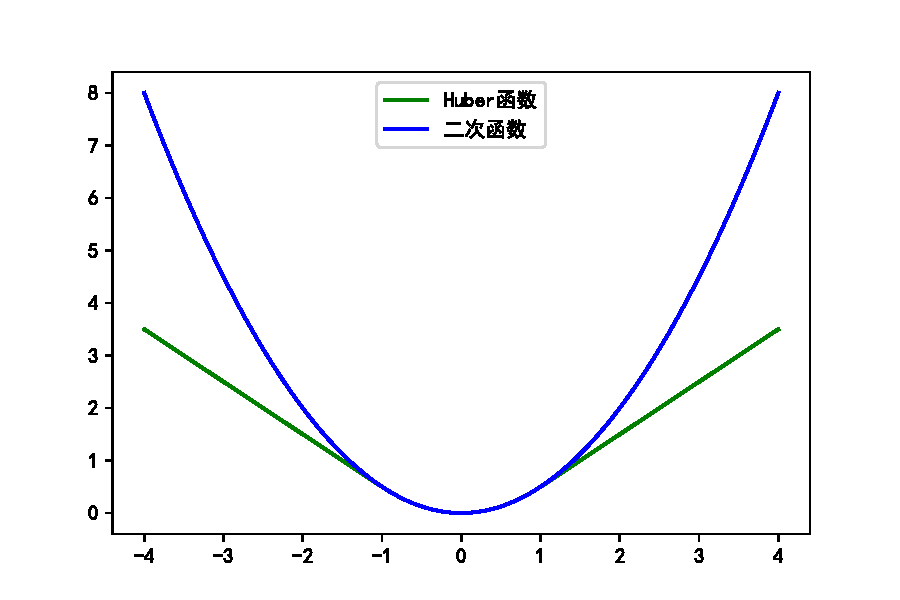
\includegraphics[width=0.45\textwidth]{figures/chapter4/fig4_1}
 	\caption{Huber函数与二次函数图像}\label{fig4_1}
 \end{figure}


需要注意的是,使用马氏范数而不是二范低于因为马氏范数消除了不同残差项的尺度不一致性(单位/量纲不一致性),或者说马氏范数对残差项的概率模型进行了归一化,从而使得不同的残差项可以直接相加。

要计算目标函数的最小值,使用迭代优化的思想,每次给优化变量一个增量,使得目标函数最小。对于IMU残差项,
\begin{equation}
\label{eqn:4.6}
\begin{aligned}
& \min _{\delta X}\left\| \mathbf{r}_\mathcal{B}(\hat{\mathbf{z}}_{b_{k+1}}^{b_k}, \mathcal{X} + \Delta \mathcal{X} )  \right\|_{P_{b_{k+1}}^{b_k}}^{2} \\
&=
\min _{\delta X} 
\left\| 
\mathbf{r}_\mathcal{B}(\hat{\mathbf{z}}_{b_{k+1}}^{b_k},\mathcal{X}) 
+ \mathbf{J}_{b_{k+1}}^{b_k} \Delta \mathcal{X}  \right\| _{P_{b_{k+1}}^{b_k}}^{2}
\end{aligned}
\end{equation}
其中,$\mathbf{J}_{b_{k+1}}^{b_k}  $ 是IMU残差项 $\mathbf{r}_{\mathcal{B}} $ 关于状态向量 $\mathcal{X} $ 的雅可比矩阵。上式可以展开成 $\mathbf{H}\Delta \mathbf{x}=\mathbf{b} $ 的形式:
\[
(\mathbf{J} _{b_{k+1}}^{b_{k}})^{T} (\mathbf{P}_{b_{k+1}}^{b_{k}})^{-1} \mathbf{J}_{b_{k+1}}^{b_{k}} \Delta \mathcal{X}
=- (\mathbf{J}_{b_{k+1}}^{b_{k}})^{T} (\mathbf{P}_{b_{k+1}}^{b_{k}})^{-1} \mathbf{r}_{B}
\]
其中,$\mathbf{P}_{b_{k+1}}^{b_k} $ 是IMU预积分中噪声项的协方差矩阵。

同理,可以写出视觉残差项的增量方程。整体目标函数的增量方程为:
\begin{equation}
\label{eqn:4.7}
\begin{aligned}
& \left( \mathbf{H}_{p}+\sum (\mathbf{J}_{b_{k+1}}^{b_{k}})^{T} (\mathbf{P}_{b_{k+1}}^{b_{k}})^{-1} \mathbf{J}_{b_{k+1}}^{b_{k}}+\sum {\mathbf{J}_{l}^{C_{j}}}^{T}  (\mathbf{P}_{l}^{C_j})^{-1}  \mathbf{J}_{l}^{C_{j}}\right) \Delta \mathcal{X} \\
& = \mathbf{b}_{p}+\sum \mathbf{J}_{b_{k+1}}^{b_{k}} (\mathbf{P}_{b_{k+1}}^{b_{k}})^{-1} \mathbf{r}_{B}+\sum {\mathbf{J}_{l}^{C_{j}} }^T  (\mathbf{P}_{l}^{C_j})^{-1}  \mathbf{r}_{C}
\end{aligned}
\end{equation}
其中,$\mathbf{P}_{l}^{C_{j}} $ 是视觉噪声的协方差。暂时不考虑先验信息,用 $(\mathbf{H}_p, \mathbf{b}_p) $ 表示。称 ${\mathbf{P}_{b_{k+1}}^{b_{k}}}^{-1} $ 为信息矩阵,其大小可以代表IMU测量数据的可靠程度,越大代表越可靠,越小代表越不可靠。可以观察到,IMU噪声越大,信息矩阵就越小,此时IMU观测量就越不可靠,可以直观的理解为目标函数“更加相信”视觉的观测量。

将增量方程(\ref{eqn:4.7})简化为:
\begin{equation}
\label{eqn:4.8}
\setlength{\abovedisplayskip}{6pt}
\setlength{\belowdisplayskip}{6pt}
\left( \bm{\Lambda}_{p}+\bm{\Lambda}_{\mathcal{B}}+\bm{\Lambda}_{\mathcal{C}} \right) \Delta \mathcal{X}=\mathbf{b}_{p}+\mathbf{b}_{\mathcal{B}}+\mathbf{b}_{\mathcal{C}}
\end{equation}
其中,$\bm{\Lambda}_{p}, \bm{\Lambda}_{\mathcal{B}}, \bm{\Lambda}_{\mathcal{C}} $ 分别为先验残差项,IMU残差项和视觉残差项的海森(Hessian)矩阵。
\subsection{IMU约束}
考虑滑动窗口中连续两帧图像( $b_{k} $和 $b_{k+1} $)内的IMU测量,根据式(3.41)中定义的IMU测量模型,预积分残差可以定义为:
\begin{equation}
\label{eqn:4.9}
\begin{split}
\mathbf{r}_\mathcal{B}(\hat{\mathbf{z}}_{b_{k+1}}^{b_k},\mathcal{X})=\begin{bmatrix} \delta\bm{\alpha}_{b_{k+1}}^{b_k} \\ \delta\bm{\beta}_{b_{k+1}}^{b_k} \\ \delta\bm{\theta}_{b_{k+1}}^{b_k} \\ \delta\mathbf{b}_a \\ \delta\mathbf{b}_g  \end{bmatrix}  
=\begin{bmatrix}
\mathbf{R}_w^{b_k}(\mathbf{p}_{b_{k+1}}^w-\mathbf{p}_{b_k}^w+\frac{1}{2}\mathbf{g}^w\Delta t_k^2-\mathbf{v}_{b_k}^w\Delta t_k)-\hat{\bm{\alpha}}_{b_{k+1}}^{b_k} \\
\mathbf{R}_w^{b_k}(\mathbf{v}_{b_{k+1}}^w+\mathbf{g}^w\Delta t_k^2-\mathbf{v}_{b_k}^w)-\hat{\bm{\beta}}_{b_{k+1}}^{b_k} \\
2\left[ {\mathbf{q}_{b_k}^w}^{-1}\otimes\mathbf{q}_{b_{k+1}}^w\otimes(\hat{\bm{\gamma}}_{b_{k+1}}^{b_k})^{-1} \right]_{xyz} \\ \mathbf{b}_{ab_{k+1}}-\mathbf{b}_{ab_k} \\
\mathbf{b}_{wb_{k+1}}-\mathbf{b}_{wb_k}
\end{bmatrix}
\end{split}
\end{equation}
其中,$[\cdot]_{x y z}$ 表示四元数的向量。$\delta \boldsymbol{\theta}_{b_{k+1}}^{b_{k}}$ 是四元数对应的三维误差状态。$\left[\hat{\boldsymbol{\alpha}}_{b_{k+1}}^{b_{k}}, \hat{\boldsymbol{\beta}}_{b_{k+1}}^{b_{k}}, \hat{\gamma}_{b_{k+1}}^{b_{k}}\right]^{T}$ 是在两个连续图像帧之间的间隔时间内带有噪声的预积分IMU测量项。$\delta \mathbf{b}_a, \delta \mathbf{b}_g $ 是加速度计bias和陀螺仪bias的误差。

IMU残差项的优化变量为:
\[
\setlength{\abovedisplayskip}{6pt}
\setlength{\belowdisplayskip}{6pt}
\left[ \mathbf{ p}_{b_{k}}^{w}, 
\mathbf{ q}_{b_{k}}^{w}\right],
\left[\mathbf{ v}_{b_{k}}^{w}, 
\mathbf{ b}_{a_{k}}, \mathbf{ b}_{\omega_{k}}\right], 
\left[\mathbf{ p}_{b_{k+1}}^{w}, \mathbf{q}_{b_{k+1}}^{w}\right],
\left[\mathbf{ v}_{b_{k+1}}^{w}, \mathbf{ b}_{a_{k+1}}, \mathbf{b}_{\omega_{k+1}}\right]
\]

在进行迭代优化时需要知道残差项对优化变量的一阶导数,也就是雅可比矩阵,以及协方差矩阵。仍旧采用扰动模型求导,扰动为:
\[
\setlength{\abovedisplayskip}{6pt}
\setlength{\belowdisplayskip}{6pt}
\left[\delta \mathbf{p}_{b_{k}}^{w},   \delta \bm{\theta}_{b_{k}}^{w}\right], 
\left[\delta \mathbf{v}_{b_{k}}^{w},   \delta \mathbf{b}_{a_{k}}, \delta \mathbf{b}_{\omega_{k}}\right], 
\left[\delta \mathbf{p}_{b_{k+1}}^{w}, \delta \bm{\theta}_{b_{k+1}}^{w}\right],
\left[\delta \mathbf{v}_{b_{k+1}}^{w}, \delta \mathbf{b}_{a_{k+1}}, \delta \mathbf{b}_{\omega_{k+1}}\right]
\]

这里直接给出通过扰动模型求导后的雅可比矩阵:
\begin{equation}
\label{eqn:4.10}
\begin{aligned}
\mathbf{J}[0]^{15 \times 7} &= \left[\frac{\partial \mathbf{r}_{\mathcal{B}}}{\partial \mathbf{p}_{b_{k}}^{w}}, \frac{\partial \mathbf{r}_{\mathcal{B}}}{\partial \mathbf{q}_{b_{k}}^{w}}\right] \\
&= \left[\begin{array}{cc}
-\mathbf{R}_{w}^{b_{k}} & \left[ \mathbf{R}_{w}^{b_{k}}\left(\mathbf{p}_{b_{k+1}}^{w} - \mathbf{p}_{b_{k}}^{w} - \mathbf{v}_{b_{k}}^{w} \Delta t_{k}+\frac{1}{2} \mathbf{g}^{w} \Delta t_{k}^{2}\right) \right]_\times \\ 
0                       & -{\left[ (\mathbf{q}_{b_{k+1}}^{w})^{-1} \otimes \mathbf{q}_{b_{k}}^{w}\right]}_L {\left[\bm{\gamma}_{b_{k+1}}^{b_{k}}\right]}_R \\
0                       & \left[ \mathbf{R}_{w}^{b_{k}}\left(\mathbf{v}_{b_{k+1}}^{w} - \mathbf{v}_{b_{k}}^{w} + \mathbf{g}^{w} \Delta t_{k}\right) \right]_\times \\
0                       & 0 \\
0                       & 0
\end{array}\right]
\end{aligned}
\end{equation}
\begin{equation}
\label{eqn:4.11}
\begin{aligned}
\mathbf{J}[1]^{15 \times 9} &= \left[\frac{\partial \mathbf{r}_{\mathcal{B}}}{\partial \mathbf{v}_{b_{k}}^{w}}, \frac{\partial \mathbf{r}_{\mathcal{B}}}{\partial \mathbf{b}_{k}}, \frac{\partial \mathbf{r}_{\mathcal{B}}}{\partial \mathbf{b}_{w_{k}}}\right] \\
&= \left[ \begin{array}{ccc}
{-\mathbf{R}_{w}^{b_{k}} \Delta t} & {-\mathbf{J}_{b_{a}}^{\alpha}} & {-\mathbf{J}_{b_{\omega}}^{\alpha}} \\ 
{0} & {0} & {\left[{\mathbf{q}_{b_{k+1}}^{w}}^{-1} \otimes \mathbf{q}_{b_{k}}^{w} \otimes \bm{\gamma}_{b_{k+1}}^{b_{k}}\right]_L \mathbf{J}_{b_{\omega}}^{\gamma}} \\ 
{-\mathbf{R}_{w}^{b_{k}}} & {-\mathbf{J}_{b_{a}}^{\beta}} & {-\mathbf{J}_{b_{\omega}}^{\beta}} \\ 
{0} & {-\mathbf{I}} & {0} \\ {0} & {0} & {\mathbf{-}I}\end{array}\right]
\end{aligned}
\end{equation}
\begin{equation}
\label{eqn:4.12}
\begin{aligned}
\mathbf{J}[2]^{15 \times 7} = \left[\frac{\partial \mathbf{r}_{\mathcal{B}}}{\partial \mathbf{p}_{b_{k+1}}^{w}}, \frac{\partial \mathbf{r}_{\mathcal{B}}}{\partial \mathbf{q}_{b_{k+1}}^{w}}\right] 
= \left[ \begin{array}{cc}
\mathbf{R}_{w}^{b_k} & {0} \\ 
{0} & \left[{\bm{\gamma}_{b_{k+1}}^{b_{k}}}^{-1} \otimes \mathbf{q}_{b_{k}}^{w-1} \otimes \mathbf{q}_{b_{k+1}}^{w}\right]_L \\ 
{0} & {0}  \\ 
{0} & {0} 
\end{array}\right]
\end{aligned}
\end{equation}
\begin{equation}
\label{eqn:4.13}
\mathbf{J}[3]^{15 \times 9}=\left[\frac{\partial \mathbf{r}_{\mathcal{B}}}{\partial \mathbf{v}_{b_{k+1}}^{w}}, \frac{\partial \mathbf{r}_{\mathcal{B}}}{\partial \mathbf{b}_{a_{k+1}}}, \frac{\partial \mathbf{r}_{\mathcal{B}}}{\partial \mathbf{b}_{w_{k+1}}}\right]
=\left[ \begin{array}{ccc}{0} & {0} & {0} \\ {0} & {0} & {0} \\ {\mathbf{R}_{w}^{b_{k}}} & {0} & {0} \\ {0} & {I} & {0} \\ {0} & {0} & {\mathbf{I}}\end{array}\right]
\end{equation}

协方差矩阵是\ref{chap:3.2.3}小节中研究的预积分中的IMU增量误差的协方差矩阵,即公式(\ref{eqn:3.56})。
\subsection{视觉约束}
考虑第  $l$ 个特征,其对应的3D空间点为 $\mathbf{P}_l^{w} $ ,该特征在第 $i$  幅图像中被第一次观测到,观测到的像素坐标为 $ \mathbf{P}_{uv_{i}} =[u_l^{c_i},u_l^{c_j}]^{T} $ 。
\begin{equation}
\label{eqn:4.14}
\setlength{\abovedisplayskip}{6pt}
\setlength{\belowdisplayskip}{6pt}
\mathbf{P}_{uv_{i}}  =\lambda_{l} \pi_{c}\left( \mathbf{T}_{b \leftarrow c}^{-1} \mathbf{T}_{w \leftarrow b_{i}}^{-1} \mathbf{P}^w_{l}\right)
\end{equation}
其中,$\pi_{c} $ 将世界坐标点映射为像素坐标点,$\mathbf{T}_{b \leftarrow c}^{-1} $ 将坐标从IMU系变换到相机系,$\mathbf{T}_{w \leftarrow b_{i}}^{-1} $ 将世界坐标系下的坐标变换到IMU坐标系下。$\lambda_l $ 是第 $l$ 个特征在第 $i$ 幅图像下的逆深度。由式(\ref{eqn:4.14})可得,
\begin{equation}
\label{eqn:4.15}
\begin{aligned}
\mathbf{P}^w_{l} &= \mathbf{T}_{w\leftarrow b_{i}} \mathbf{T}_{b\leftarrow c} \frac{1}{\lambda_{l}} \pi_{c}^{-1}\left( \mathbf{P}_{uv_{i}} \right) \\
&= \mathbf{R}_{b_{i}}^{w}\left(\mathbf{R}_{c}^{b} \frac{1}{\lambda_{l}} \pi_{c}^{-1}
\left(\left[ \begin{array}
{c}{u_{l}^{c_{i}}} \\ {v_{l}^{c_{i}}}
\end{array}\right]\right)
+ \mathbf{p}_{c}^{b}\right)+\mathbf{p}_{b_{i}}^{w}
\end{aligned}
\end{equation}
 $\mathbf{P}_l^{w} $ 在第 $j$ 副图像对应的相机坐标系下的坐标为,
\begin{equation}
\label{eqn:4.16}
\setlength{\abovedisplayskip}{6pt}
\setlength{\belowdisplayskip}{6pt}
\mathcal{ P}_{l}^{c_{j}}=\mathbf{T}_{b \leftarrow c}^{-1} \mathbf{T}_{w \leftarrow b_{j}}^{-1} \mathbf{P}_{l}^{w}
\end{equation}
进而得到,
\begin{equation}
\label{eqn:4.17}
\begin{aligned}
\mathbf{ P}_{l}^{w} &= \mathbf{T}_{w \leftarrow b_{j}} \mathbf{T}_{b \leftarrow c} \mathcal{P}_{l}^{c_{j}} \\
&= \mathbf{R}_{b_{j}}^{w}\left(\mathbf{R}_{c}^{b} \mathcal{P}_{l}^{c_{j}}+\mathbf{p}_{c}^{b}\right)+\mathbf{p}_{b_{j}}^{w}
\end{aligned}
\end{equation}
联立式(\ref{eqn:4.15})和(\ref{eqn:4.17})可得,
\begin{equation}
\label{eqn:4.18}
\mathcal{P}_l^{c_j}=\mathbf{R}_b^c(\mathbf{R}_w^{b_j}(\mathbf{R}_{b_i}^w(\mathbf{R}_c^b\frac{1}{\lambda_l}{\pi_c}^{-1}(\begin{bmatrix}  u_l^{c_j} \\ v_l^{c_j}
\end{bmatrix})+\mathbf{p}_c^b)+\mathbf{p}_{b_i}^w-\mathbf{p}_{b_j}^w)-\mathbf{p}_c^b)
\end{equation}

此时,可以定义该特征在第 $j$ 幅图像中的观测点和重投影点之间的残差定义为:
\begin{equation}
\label{eqn:4.19}
\mathbf{r}_\mathcal{C}(\hat{\mathbf{z}}_l^{c_j},\mathcal{X})= 
\hat{\bar{\mathcal{P}}}_l^{c_j}-\frac{ \mathcal{P}_l^{c_j} }{\left\|\mathcal{P}_l^{c_j}\right\|}
\end{equation}
其中,$\mathcal{P}_l^{c_j} $ 为 $\mathbf{P}_l^{w} $ 在第 $j$ 副图像上对应的归一化平面坐标,
\begin{equation}
\label{eqn:4.20}
\hat{\bar{\mathcal{P}}}_l^{c_j}={\pi_c}^{-1}
(\begin{bmatrix}  \hat{u}_l^{c_j} \\ \hat{v}_l^{c_j}
\end{bmatrix})
\end{equation}
视觉残差项的优化变量为:
\[
\setlength{\abovedisplayskip}{6pt}
\setlength{\belowdisplayskip}{6pt}
\left[ \mathbf{p}_{b_{i}}^{w}, \mathbf{q}_{b_{i}}^{w}\right], 
\left[ \mathbf{p}_{b_{j}}^{w}, \mathbf{q}_{b_{j}}^{w}\right], 
\left[ \mathbf{p}_{c}^{b}, \mathbf{q}_{c}^{b}\right], 
\lambda_{l}
\]

同样需要计算残差项关于这些优化变量的一阶导数,得到其雅可比矩阵。这里直接给出各优化变量的雅可比矩阵:
\begin{equation}
\label{eqn:4.21}
\left\{
\begin{aligned}
\mathbf{ J}[0]^{3 \times 7} &= \left[\frac{\partial \mathbf{r}_{\mathcal{C}}}{\partial \mathbf{p}_{b_{i}}^{w}}, \frac{\partial \mathbf{r}_{\mathcal{C}}}{\partial \mathbf{q}_{b_{i}}^{w}}\right]
=\left[\mathbf{R}_{b}^{c} \mathbf{R}_{w}^{b_{j}}-\mathbf{R}_{b}^{c} \mathbf{R}_{w}^{b_{j}} \mathbf{R}_{b_{i}}^{w}\left[\mathbf{R}_{c}^{b} \frac{1}{\lambda_{l}} \hat{\bar{\mathcal{P}}}_{l}^{c_{i}}+\mathbf{p}_{c}^{b}\right]_\times\right] \\
\mathbf{J}[1]^{3 \times 7}&=\left[\frac{\partial \mathbf{r}_{\mathcal{C}}}{\partial \mathbf{p}_{b_{j}}^{w}}, \frac{\partial \mathbf{r}_{\mathcal{C}}}{\partial \mathbf{q}_{b_{j}}^{w}}\right] \\
&=\left[-\mathbf{R}_{b}^{c} \mathbf{R}_{w}^{b_{j}} \mathbf{R}_{b}^{c}\left[\mathbf{R}_{w}^{b_{j}}\left[\mathbf{R}_{b_{i}}^{w}\left(\mathbf{R}_{c}^{b} \frac{\hat{\bar{P}}_{l}^{c_{i}}}{\lambda_{l}}+\mathbf{p}_{c}^{b}\right)+\mathbf{p}_{b_{i}}^{w}-\mathbf{p}_{b_{j}}^{w}\right]\right]_\times\right] \\
\mathbf{J}[2]^{3 \times 7} &= \left[\frac{\partial \mathbf{r}_{\mathcal{C}}}{\partial \mathbf{p}_{\mathcal{C}}^{b}}, \frac{\partial \mathbf{r}_{\mathcal{C}}}{\partial \mathbf{q}_{c}^{b}}\right] \\
&= \left[ \begin{array}
{c}{\mathbf{R}_{b}^{c}\left(\mathbf{R}_{w}^{b_{j}} \mathbf{R}_{b_{i}}^{w}-\mathbf{I}_{3 \times 3}\right)} \\ 
\begin{aligned}
&{-\mathbf{R}_{b}^{c} \mathbf{R}_{w}^{b_{j}} \mathbf{R}_{b_{i}}^{w} \mathbf{R}_{c}^{b} \left[\frac{\hat{\bar{\mathcal{P}}}_{l}^{c_{i}}}{\lambda_{l}}\right]_\times
	+\left[\mathbf{R}_{b}^{c} \mathbf{R}_{w}^{b_{j}} \mathbf{R}_{b_{i}}^{w} \mathbf{R}_{c}^{b} \frac{\hat{\bar{\mathcal{P}}}_{l}^{c_{i}}}{\lambda_{l}}\right]_\times} \\
	&{+\left[\mathbf{R}_{b}^{c}\left[\mathbf{R}_{w}^{b_{j}}\left(\mathbf{R}_{b_{i}}^{w} \mathbf{p}_{c}^{b}+\mathbf{p}_{b_{i}}^{w}-\mathbf{p}_{b_{j}}^{w}\right)-\mathbf{p}_{c}^{b}\right]\right]_\times}
\end{aligned} \\
\end{array}\right]^{T} \\
\mathbf{J}[3]^{3 \times 1} &=\frac{\partial \mathbf{r}_{\mathcal{C}}}{\partial \lambda_{l}}=-\mathbf{R}_{b}^{c} \mathbf{R}_{w}^{b_{j}} \mathbf{R}_{b_{i}}^{w} \mathbf{R}_{c}^{b} \frac{\hat{\bar{P}}_{l}^{c_{i}}}{\lambda_{l}^{2}}
\end{aligned}
\right.
\end{equation}
\subsection{边缘化}
前面在研究残差项的时候,忽略了先验残差项,这个先验残差项就是通过边缘化(Marginalization)\upcite{Paz2008Divide}来的。整个后端是基于滑动窗口来进行非线性优化的,滑动窗口内的图像帧数量是固定的(在实际工程中取10帧),这样会带来一个问题:窗口在向前滑动的过程中,总会有新的图像帧和路标点进来,而窗口中最旧的图像帧和路标点会滑出窗口。要对滑窗内的所有图像位姿及其路标点进行优化,那么不能直接将最旧的图像帧及其观测到的路标点直接删除,因为这样会丢失观测信息,降维约束项。那么怎么才能在不减少约束项的情况下丢掉最旧的图像帧及其路标点呢?边缘化就是用来解决此问题的。

(1)舒尔补消元

采用高斯牛顿或者LM方法进行非线性优化时,每次迭代都需要求解增量方程 $\mathbf{H}\delta \mathbf{x}=\mathbf{b} $ ,将 $\mathbf{H}\delta \mathbf{x}=\mathbf{b} $ 写为:
\begin{equation}
\label{eqn:4.22}
\left[ \begin{array}{cc}
{\bm{\Lambda}_{a}} & {\bm{\Lambda}_{b}} \\ 
{\bm{\Lambda}_{b}^{T}} & {\bm{\Lambda}_{c}}
\end{array}\right] 
\left[ \begin{array}{c}
{\delta \mathbf{x}_{1}} \\ {\delta \mathbf{x}_{2}}
\end{array}\right]
=\left[ \begin{array}
{l}{\mathbf{b}_{1}} \\ {\mathbf{b}_{2}}
\end{array}\right]
\end{equation}
其中,$\delta \mathbf{x}_1 $ 是想要边缘化掉的优化变量,$\delta \mathbf{x}_2 $ 是与 $\delta \mathbf{x}_1 $ 有约束关系的想要保留的优化变量。定义舒尔项\upcite{sibley2010sliding}:
\begin{equation}
\label{eqn:4.23}
\left[ \begin{array}{cc}
{\mathbf{I}} & {0} \\ 
{-\bm{\Lambda}_{b}^{T} \bm{\Lambda}_{a}^{-1}} & {\mathbf{I}}\end{array}\right]
\end{equation}
将等式(\ref{eqn:4.22})两边同时乘以式(\ref{eqn:4.23}),
\begin{equation}
\label{eqn:4.24}
\begin{aligned}
\left[ \begin{array}{cc}
{ \mathbf{I}} & {0} \\ 
{-\bm{\Lambda}_{b}^{T} \bm{\Lambda}_{a}^{-1}} & {\mathbf{I}}
\end{array}\right] 
\left[ \begin{array}{cc}
{\bm{\Lambda}_{a}} & {\bm{\Lambda}_{b}} \\ 
{\bm{\Lambda}_{b}^{T}} & {\bm{\Lambda}_{c}}
\end{array}\right] 
\left[ \begin{array}{c}
{\delta \mathbf{x}_{1}} \\ {\delta \mathbf{x}_{2}}
\end{array}\right]
&=
\left[ \begin{array}{cc}
{\mathbf{I}} & {0} \\ 
{-\bm{\Lambda}_{b}^{T} \bm{\Lambda}_{a}^{-1}} & {\mathbf{I}}
\end{array}\right] 
\left[ \begin{array}
{l}{\mathbf{b}_{1}} \\ {\mathbf{b}_{2}}
\end{array}\right] \\
\Longrightarrow
\left[ \begin{array}{cc}
{\bm{\Lambda}_{a}} & {\bm{\Lambda}_{b}} \\ 
{0} & {\bm{\Lambda}_{c}-\bm{\Lambda}_{b}^{T} \bm{\Lambda}_{a}^{-1} \bm{\Lambda}_{b}}
\end{array}\right] 
\left[ \begin{array}{l}
{\delta \mathbf{x}_{1}} \\ {\delta \mathbf{x}_{2}}
\end{array}\right]
&=
\left[ \begin{array}{c}
{\mathbf{b}_{1}} \\ {\mathbf{b}_{2}-\bm{\Lambda}_{\mathbf{b}}^{T} \bm{\Lambda}_{a}^{-1} \mathbf{b}_{1}}
\end{array}\right]
\end{aligned}
\end{equation}
通过式(\ref{eqn:4.24}),可以忽略 $\delta \mathbf{x}_1$ 单独求解 $\delta \mathbf{x}_2$,
\begin{equation}
\label{eqn:4.25}
\begin{aligned}
\left( \bm{\Lambda}_{c}-\bm{\Lambda}_{b}^{T} \bm{\Lambda}_{a}^{-1} \bm{\Lambda}_{b}\right) \delta \mathbf{x}_{2} &= 
b_{2}- \bm{\Lambda}_{b}^{T} \bm{\Lambda}_{a}^{-1} \mathbf{b}_{1} \\
\Longrightarrow  \quad \quad
\mathbf{H}^{*} \delta \mathbf{x}_{2}^{*}&= \mathbf{b}^{*}
\end{aligned}
\end{equation}
式(\ref{eqn:4.25})中,$\mathbf{b}^{*} $ 是 $\bm{\Lambda}_{b}^{T} \bm{\Lambda}_{a}^{-1} \mathbf{b}_{1} $有关的函数,所以,通过舒尔补,在保留了变量 $\delta \mathbf{x}_1 $ 的约束信息的情况下消掉了$\delta \mathbf{x}_1 $ 。因此可以说式(4.25)保留了变量 的先验信息。此时可以构建先验残差项:
\begin{equation}
\label{eqn:4.26}
\setlength{\abovedisplayskip}{6pt}
\setlength{\belowdisplayskip}{6pt}
\mathbf{r}_p-\mathbf{H}_p\mathcal{X} \Longleftrightarrow 
\hat{\mathbf{b}}^{*} - \mathbf{H}^{*} \delta \mathbf{x}_{2}^{*}
\end{equation}

(2)边缘化过程

假设相机在四个不同的地方拍摄了四张图像,相机的位姿分别为 $ \mathbf{x}_{p_1},  \mathbf{x}_{p_2},  \mathbf{x}_{p_3},  \mathbf{x}_{p_4} $ ,四张图像总共观测到了六个路标点 $ \mathbf{x}_{m_1},  \mathbf{x}_{m_2}, \mathbf{x}_{m_3}, \mathbf{x}_{m_4}, \mathbf{x}_{m_5}, \mathbf{x}_{m_6}$ ,他们之间的关系如图\ref{fig4_2}所示。
\begin{figure}[h]\setlength{\belowcaptionskip}{-12pt}
	\centering
	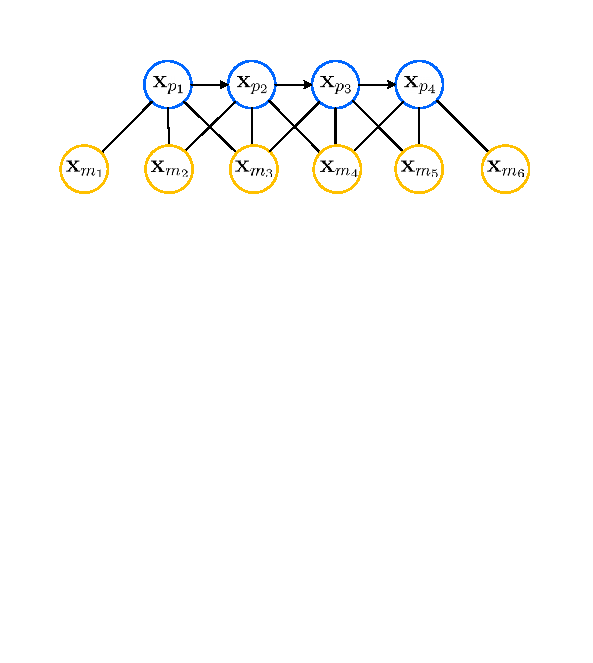
\includegraphics[width=0.15\textwidth, angle=-90]{figures/chapter4/fig4_2}
	\caption{位姿和路标点的关系}\label{fig4_2}
\end{figure}
图\ref{fig4_2}中相机和路标点之间的连线表示相机观测到了该路标点,相机和相机之间的箭头连接表示他们之间的IMU约束。

用图\ref{fig4_3}(a)表示原始的 $\mathbf{H} $ 矩阵,图中,m表示路标,p表示位姿,颜色块代表相互关联。图4.3(b)表示将 $\mathbf{H} $ 矩阵中跟位姿 $\mathbf{x}_{p_1} $ 有关的元素移至左上角。图4.3(c)表示将位姿 $\mathbf{x}_{p_1} $ 边缘化掉后的 $\mathbf{H} $ 矩阵,也就是式(\ref{eqn:4.25})中的$\left( \bm{\Lambda}_{c}-\bm{\Lambda}_{b}^{T} \bm{\Lambda}_{a}^{-1} \bm{\Lambda}_{b}\right) $ 。

观察图\ref{fig4_3}(c)可以发现,相对于图(b),图(c)更加稠密,或者说边缘化掉一个位姿后,余下的 $\mathbf{H} $ 矩阵会多出三部分颜色块(图中的黄色块)。图\ref{fig4_4}表示图\ref{fig4_3}(c)对应的关系图。
\begin{figure}[h]\setlength{\belowcaptionskip}{-12pt}
	\centering
	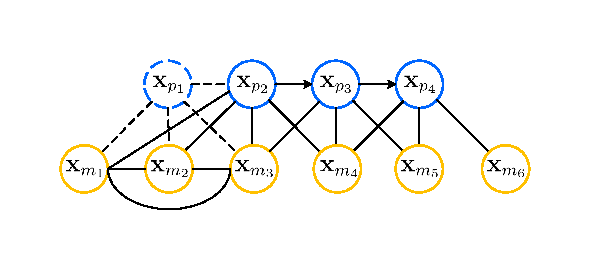
\includegraphics[width=0.15\textwidth, angle=-90]{figures/chapter4/fig4_4}
	\caption{边缘化掉 $\mathbf{x}_{p_1} $ 后位姿和路标点的关系}\label{fig4_4}
\end{figure}

观察图\ref{fig4_4}可以发现,路标点 $\mathbf{x}_{m_1},  \mathbf{x}_{m_2}, \mathbf{x}_{m_3} $ 之间已经相互有了新的联系,并且,位姿 $\mathbf{x}_{p_2} $ 与路标点 $\mathbf{x}_{m_2} $ 也有了新的联系。这些新的联系就是新的约束项,表现在图\ref{fig4_3}(c)中的黄色区域。

图\ref{fig4_3}(d)是表示再次边缘化掉路标点 $\mathbf{x}_{m_1} $ 后的 $\mathbf{H} $ 矩阵,其对应的关系图如图\ref{fig4_5}所示。
\begin{figure}[h]\setlength{\belowcaptionskip}{1pt}
	\centering
	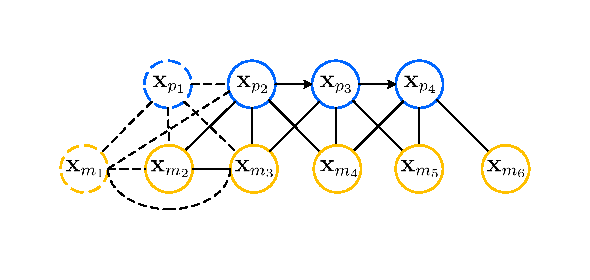
\includegraphics[width=0.15\textwidth, angle=-90]{figures/chapter4/fig4_5}
	\caption{边缘化掉 $\mathbf{x}_{p_1} $ 和$\mathbf{x}_{m_1} $ 后位姿和路标点的关系}\label{fig4_5}
\end{figure} 
\begin{figure}[h]\setlength{\belowcaptionskip}{-12pt}
	\centering
	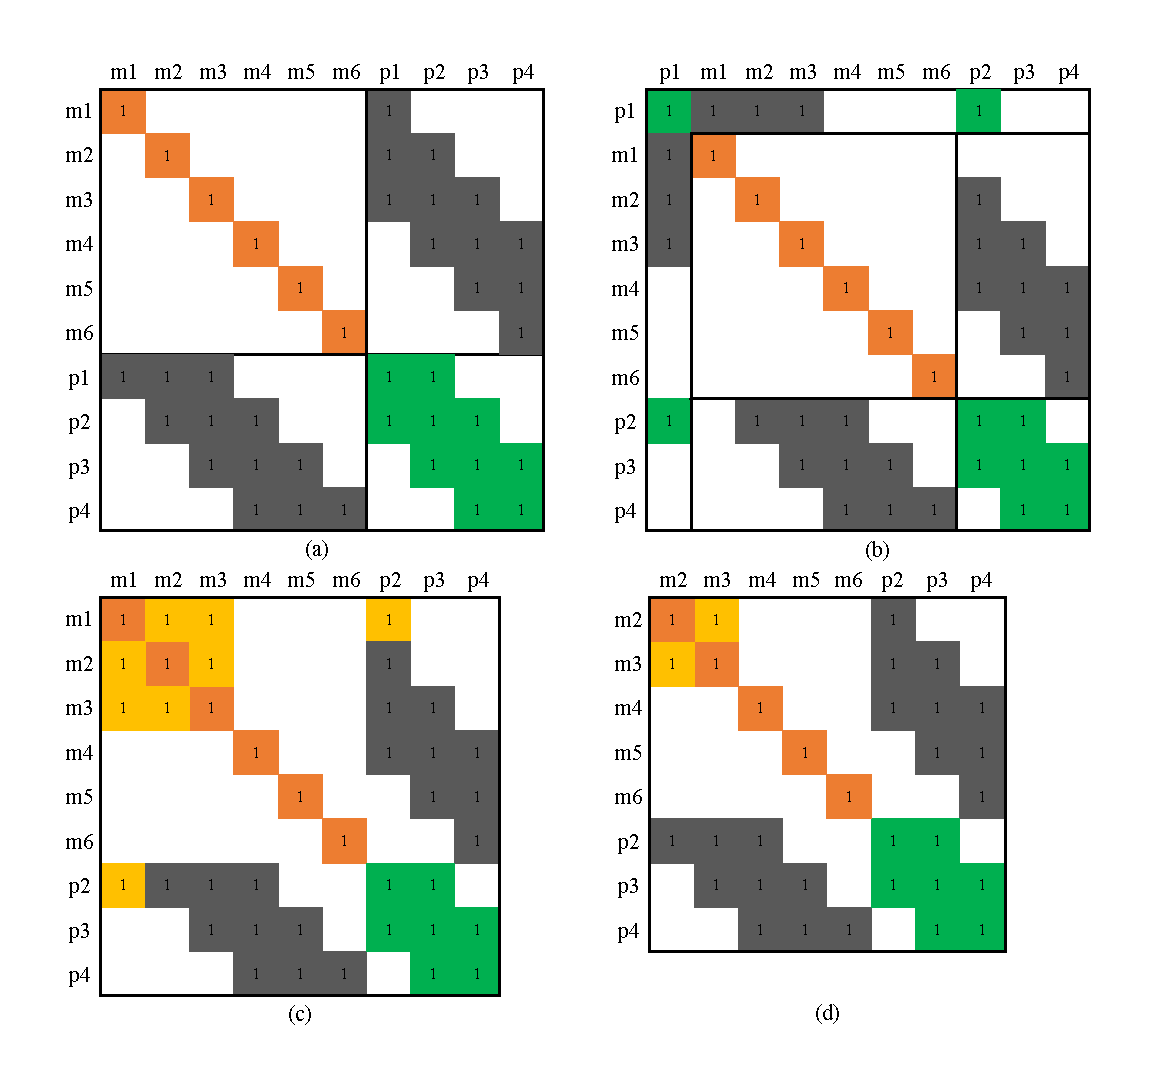
\includegraphics[width=0.75\textwidth, angle=-90]{figures/chapter4/fig4_3}
	\caption{边缘化过程中 $\mathbf{H} $ 矩阵变化图}\label{fig4_3}
\end{figure}
观察图\ref{fig4_3}(d),发现$\mathbf{H} $ 矩阵并没有变得更稠密,这是因为路标点 $\mathbf{x}_{m_1} $ 本身就没有被其他路标点观测到(从图\ref{fig4_4}中可以看出),也就不会与其他位姿产生约束关系。因此,可以得出一个结论:当边缘化掉不被其他帧所观测到的路标点时,$\mathbf{H} $ 矩阵不会进一步稠密。而对于被其他帧所观测到的路标点,通常不进行边缘化。

3. 滑窗策略
\begin{figure}[h]\setlength{\belowcaptionskip}{-12pt}
	\centering
	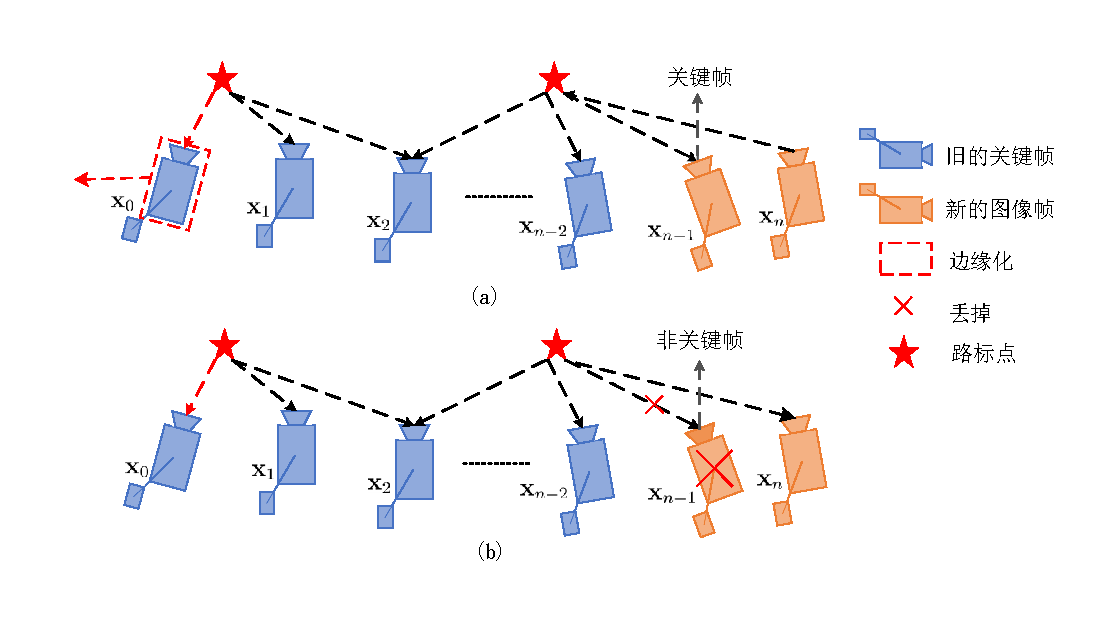
\includegraphics[width=0.4\textwidth, angle=-90]{figures/chapter4/fig4_6}
	\caption{滑动窗口示意图}\label{fig4_6}
\end{figure}

如图\ref{fig4_6}所示,整个后端非线性优化采用滑动窗口机制,窗口内维持固定的图像帧数量,根据新到来的图像帧是否为关键帧,使用不同的处理机制。图中$\mathbf{x}_n $ 为最新的图像帧, $\mathbf{x}_{n-1} $为次新帧图像,$\mathbf{x}_{n-2} $ 为第一帧旧的图像帧, $\mathbf{x}_{0} $为最旧的图像帧。

(1)如果 $\mathbf{x}_{n-1} $ 是关键帧,对 $\mathbf{x}_{0} $进行边缘化处理,与 $\mathbf{x}_{0} $及其关联的路标点的约束信息将转变为先验信息并整合到目标函数中;

(2)如果 $\mathbf{x}_{n-1} $不是关键帧,将 $\mathbf{x}_{n-1} $及其观测到的路标点直接丢弃。如果$\mathbf{x}_{n-1} $ 不是关键帧,说明它跟$\mathbf{x}_{n-2} $ 很相似(通过视差来判断是否为关键帧),那么$\mathbf{x}_{n-1} $ 及其路标点具有的约束信息和$\mathbf{x}_{n-2} $ 几乎一样,所以直接丢掉$\mathbf{x}_{n-1} $ 也不会丢失很多的约束信息。

需要注意的是,不管是边缘化还是直接丢弃图像帧,都会完整的保留图像帧所对应的IMU预积分信息,从而确保IMU预积分不中断。
\section{闭环检测}
上一章研究了前端、初始化和后端优化,此时是视觉和IMU已经构成了紧耦合的VIO系统,能够估计出自身的位姿和路标点的位置。此时的VIO系统虽然可以对自身进行定位,但是由于视觉和IMU都有不可避免的累计误差,所以在融合之后的系统还是有误差的。这就导致了系统长时间估计的结果是不可靠的,无法构建全局一致(Global Consistent)的轨迹和地图。

闭环检测算法可以检测相机是否回到了之前的位置,如果检测到闭环,算法会将之前的累计误差消除掉,将轨迹拉回正确的位置,从而构建全局一致的轨迹和地图。而且,闭环检测能够给出当前图像与之前所有图像之间的关联信息,所以,如果在前端特征跟丢的情况下,可以通过闭环检测对当前的位置进行重定位,从而不至于使系统崩溃。
\subsection{词袋模型}
闭环检测有两种思路:基于里程计的几何关系和基于外观。基于里程计的几何关系是指,当相机运动到以前走过的某个位置附近时,检测是否存在闭环\upcite{hahnel2003efficient}。这种方法有一个致命问题,长时间的视觉里程计的累计误差会导致轨迹严重漂移,相机自身是无法分辨出是否回到之前的某个位置,也就无法判断是否存在闭环关系。因此这种方法仅仅适用于短距离,短时间的闭环运动。

第二种方法是基于外观的。它仅仅依靠图像间的相似程度来确定是否存在闭环关系。这种方法不受前端累计误差的影响,使得闭环检测可以独立的作为系统的一个模块。基于外观的方法是视觉SLAM中检测闭环的主流做法,并且已经应用于多个实际系统中\upcite{ulrich2000appearance}\upcite{latif2013robust}\upcite{mur2015orb}。

如果使用第二种方法,那么闭环检测的关键就在于如何计算图像之间的相似程度。对于任意两张图像 $\bm{A} $ 和 $\bm{B} $ ,会用一种方法计算出他们之间的相似性评分:$s(\bm{A}, \bm{B}) $ 。设定一个阈值,当评分大于这个阈值的时候,就认为他们之间存在闭环关系。通常,采用词袋模型(Bag-of-Words,BoW)\upcite{filliat2007visual}\upcite{galvez2012bags}来计算相似性评分。

词袋是用来描述图像内容特征的方法。图像中出现的一类物体(比如车,房子,人等)会对应于词袋中的一个“单词”,所有的单词构成一个“字典”。通常找出图像中出现了那些“单词”,出现单词的地方用“1”表示,没有出现的用“0”表示,所有的单词出现情况会构成一个向量,然后用这个向量来描述这张图像。最后,用向量的相似程度来表示图像间的相似程度。

假如有一个“字典”,字典里面的单词包括:“汽车”,“行人”和“房子”,分别记为$w_1,w_2,w_3 $ 。有一副图像 $\bm{A} $ 包含了“汽车”和“行人”,没有“房子”,图像$\bm{B} $ 包含了“汽车”和“房子”,没有“行人”那么 $\bm{A},\bm{B} $ 可以表示为:
\begin{equation}
\label{eqn:4.27}
\setlength{\abovedisplayskip}{6pt}
\setlength{\belowdisplayskip}{6pt}
\begin{aligned}
\bm{A}&=1 \cdot w_{1}+1 \cdot w_{2}+0 \cdot w_{3}, \\
\bm{B}&=1 \cdot w_{1}+0 \cdot w_{2}+1 \cdot w_{3}
\end{aligned}
\end{equation}

所以,可以用向量 $[1,1,0]^{T} $ 来表示图像 $\bm{A} $ ,向量$[1,0,1]^{T} $ 来表示图像 $\bm{B} $。可以发现,词袋模型描述的是图像中是否存在某个物体,而不管他们出现在图像的哪个地方。根据这两个向量来计算相似性:
\begin{equation}
\label{eqn:4.28}
\setlength{\abovedisplayskip}{6pt}
\setlength{\belowdisplayskip}{6pt}
s(\boldsymbol{A}, \boldsymbol{B})=1-\frac{1}{W}\|\boldsymbol{A}-\boldsymbol{B}\|_{1}
\end{equation}
其中, $W $是词袋中“单词”的个数,这里 $W =3$,当然,实际中的 $W $会大得多。 $||\cdot || $代表$L_1 $ 范数,也可以选用其他范数,依据具体情况而定。可以发现,当向量 $\bm{A},\bm{B} $ 完全一样时,$s=1$ ;完全相反时,$s=0$ 。这样就可以用 $s$ 的大小来描述图像的相似性了。
\subsection{字典构建}
字典是由“单词”构成,而单词是从图像中抽象而来的。一个“单词”往往是一类特征的集合,所以可以通过聚类(Clustering)来确定“单词”。

聚类属于无监督机器学习(Unsupervised ML),用来寻找大量数据中的规律。假设在前端提取了 $N$个特征,想要从这$N$ 个特征中抽象出来$k$ 个“单词”。使用K均值(K-means)\upcite{jain2010data}算法来解决该问题:

(1)在 $N$ 个特征中随机选取 $k$ 个特征作为中心点:$c_{1}, \dots, c_{k} $ ;

(2)对其他的每个特征,计算它和每个中心点之间的距离,将它与距离最小的那个中心点归为一类;

(3)再次计算每个类的中心点;

(4)如果重新计算出来的中心点和之前的中心点相差不大,则说明算法收敛,聚类成功。否则,返回到步骤(1)。

至此,就可以得到一个字典了。接下来要考虑的是如何根据图像中提取的特征和字典中的“单词”进行匹配。最简单的方法是采取暴力匹配,将特征和字典中的每个“单词”进行匹配,取相似度最高的那个。然而,字典一般是通用性的,这就意味着字典中含有很多的单词,暴力匹配会很耗时。

为了解决这个问题,将字典表示称 $k$ 叉树。$k$ 叉树将聚类层次化,是k均值的一种扩展。如图\ref{fig4_7}所示,用刚才的 $N$ 个特征构建一个深度为 $d$ ,树杈为 $k$ 的树:

(1)用k均值法将根节点(所有的 $N$ 个特征)聚成 $k$ 类,得到第一层聚类;

(2)对第一层聚类的每个节点,再使用k均值法聚成 $k$ 类,得到第二层聚类;

(3)以此类推,直到第 $k-1$ 层聚类,也就是叶子节点,此时的每个叶子节点就是一个“单词”。

可以发现深度为 $d$ ,分支为 $k$ 的树,可以最终聚类成 $k^d$ 个单词。在查找“单词”时,只需要查找每一个中间层聚类的聚类中心,总共需要查找 $d$ 次。
\begin{figure}[h]\setlength{\belowcaptionskip}{-12pt}
	\centering
	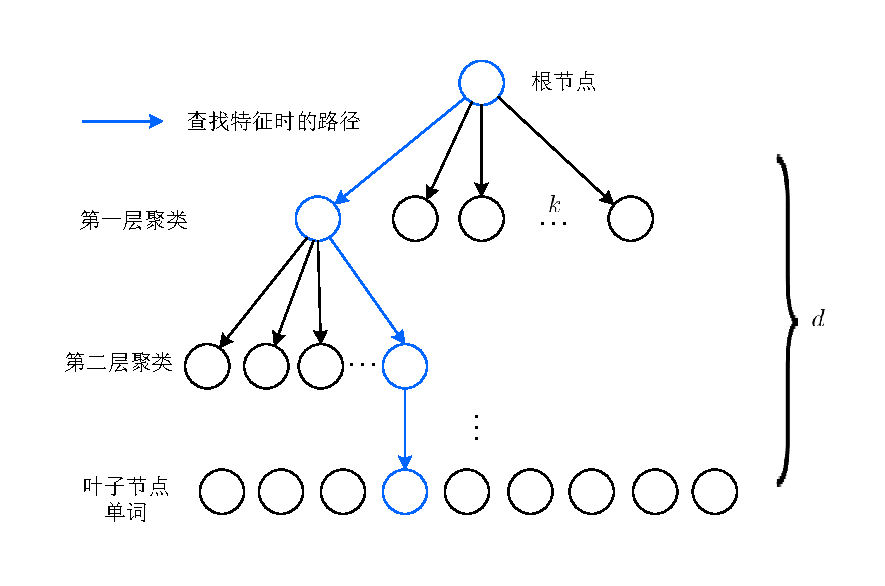
\includegraphics[width=0.4\textwidth, angle=-90]{figures/chapter4/fig4_7}
	\caption{K叉树字典示意图}\label{fig4_7}
\end{figure}
\subsection{相似度计算}
在研究词袋模型的时候简单研究了一种计算相似度的方法,那是一种简单的为了帮助理解的方法。实际中,会用到另一种方法。在之前研究的计算方法中,对所有的“单词”都同等对待,有就是“1”,没有就是“0”。但是,实际中,不同的“单词”在区分性上不相同。比如,在空旷的野外,像“树木”,“花草”,“高山”等类的“单词”会在图像中经常出现,无法根据他们判断该图像跟其他图像的区别。但是如果有“房屋”,“汽车”等类的“单词”出现时,将更容易的判断出该图像相对于其他图像的独特之处。可以说,他们提供了区分度更大的信息。所以,需要对每个单词的区分度有一个量化的评估,通常使用加权的方法来区别不同单词的重要性。权重越大,区分度就越高。

在文本检索领域,TF-IDF(Term Frequency–Inverse Document Frequency)是一种常见的方法\upcite{sivic2003video}\upcite{robertson2004understanding}。TF表示,如果文本中经常出现一个单词,则它的区分度相对较好。IDF表示,文本中出现的相似单词越少,与其他文本的区别就越大。在闭环检测中可以借鉴此方法。

对于词袋模型,在构建词典时,借鉴IDF思想。计算某个“单词” $w_i$ 中的特征数量与所有特征总数的比值,将这个比值作为IDF。设 $w_i$ 的特征数量为 $n_i$ ,特征总数为 $n$ ,那么 $w_i$ 的IDF为:
\begin{equation}
\label{eqn:4.29}
\setlength{\abovedisplayskip}{6pt}
\setlength{\belowdisplayskip}{6pt}
\mathrm{IDF}_{i}=\log \frac{n}{n_{i}}
\end{equation}
另一方面,对于单个图像,借鉴TF思想。设图像 $\bm{A} $ 中,“单词” $w_i$ 出现了 $m_i$ 次,出现的单词总数为 $m$ ,那么 $w_i$ 的TF为:
\begin{equation}
\label{eqn:4.30}
\setlength{\abovedisplayskip}{6pt}
\setlength{\belowdisplayskip}{6pt}
\mathrm{TF}_{i}=\frac{m_{i}}{m}
\end{equation}
定义 $w_i$ 的权重为:
\begin{equation}
\label{eqn:4.31}
\setlength{\abovedisplayskip}{6pt}
\setlength{\belowdisplayskip}{6pt}
\eta_{i}=\mathrm{TF}_{i} \times \operatorname{IDF}_{i}
\end{equation}
有了每个“单词”的权重,可以计算该图像的词袋(用向量 $\bm{v}_A $ 表示):
\begin{equation}
\label{eqn:4.32}
\setlength{\abovedisplayskip}{6pt}
\setlength{\belowdisplayskip}{6pt}
\bm{v}_{A}  \triangleq 
\left\{\left(w_{1}, \eta_{1}\right),\left(w_{2}, \eta_{2}\right), \ldots,\left(w_{N}, \eta_{N}\right)\right\}
\end{equation}
 $\bm{v}_A $是一个稀疏向量,其非零部分(TF-IDF的值)表示图像中包括哪些“单词”。
 
 假设计算出了图像 $\bm{A} $ 和 $\bm{B} $ 的词袋: $\bm{v}_A $和$\bm{v}_B $ ,那么可以定义他们之间的相似度为:
 \begin{equation}
 \label{eqn:4.33}
 s\left(\boldsymbol{v}_{A}-\boldsymbol{v}_{B}\right)=2 \sum_{i=1}^{N}\left|\boldsymbol{v}_{A i}\right|+\left|\boldsymbol{v}_{B i}\right|-\left|\boldsymbol{v}_{A i}-\boldsymbol{v}_{B i}\right|
  \end{equation}
  当然相似度的计算方法有很多种,这里采用 $L_1 $ 范数形式。
  
  在滑动窗口策略中,会实时计算当前帧与字典里词袋的相似度分数,并与之前的所有关键帧进行比较,并对其实施闭环一致性检验,从而得到闭环候选帧。  
\section{重定位和闭环优化}
\subsection{重定位}
在后端采用的滑动窗口和边缘化方案极大的降低了计算的复杂性,但也给系统带来了累积误差。更确切地说,累积误差主要发生在全局三维位置 $(x,y,z) $ 和与重力方向垂直的偏航角上。为了减少误差,提出了一种利用闭环检测来矫正误差图像位置的重定位方法。

如图\ref{fig4_8}所示,通过闭环检测建立闭环候选帧(蓝色的帧)和当前滑动窗口中的图像帧(绿色的帧)之间的特征关系。当检测到闭环时,将当前帧的位姿及其对应的路标点作为视觉约束项,并添加到目标函数中。所以式(4.2)可以重新写为:
 \begin{equation}
\label{eqn:4.34}
\begin{split}
\underset{\mathcal{X}}{\text{min}}\left\{\left\| \mathbf{r}_p-\mathbf{H}_p\mathcal{X} \right\|^2+
\sum_{k\in\mathcal{B}}\left\| \mathbf{r}_\mathcal{B}(\hat{\mathbf{z}}_{b_{k+1}}^{b_k},\mathcal{X}) \right\|
_{\mathbf{p}_{b_{k+1}}^{b_k}}^2 \right.  + 
\sum_{(l,j)\in\mathcal{C}}\rho(\left\| \mathbf{r}_\mathcal{C}(\hat{\mathbf{z}}_l^{c_j},\mathcal{X}) 
\right\|_{\mathbf{p}_l^{c_j}}^2) \\ + 
\left.\sum_{(l,j)\in\mathcal{L}}\rho(\left\|\mathbf{r}_\mathcal{C}(\hat{\mathbf{z}}_l^v,\mathcal{X},\hat{\mathbf{q}}_v^w,\hat{\mathbf{p}}_v^w) \right\|_{\mathbf{p}_l^{c_v}}^2) \right\}
\end{split}
\end{equation}
其中, $(\hat{\mathbf{q}}_v^w,\hat{\mathbf{p}}_v^w) $ 是回环帧的姿态,被视为常数。$\mathcal{L} $ 是闭环帧中检索到的路标点的集合。$(l,v) $ 是指在闭环帧 $v $ 中观察到的第 $l $ 个特征。注意,虽然目标函数与之前略有不同,但待解状态量的维数保持不变,因为回环帧的姿态被视为常数。当滑动窗口建立多个回环时,使用来自所有闭环帧及其对应的路标点进行优化。这就为重新定位提供了多视角的约束,从而提高了定位的精度和平滑性。
\begin{figure}[h]\setlength{\belowcaptionskip}{-12pt}
	\centering
	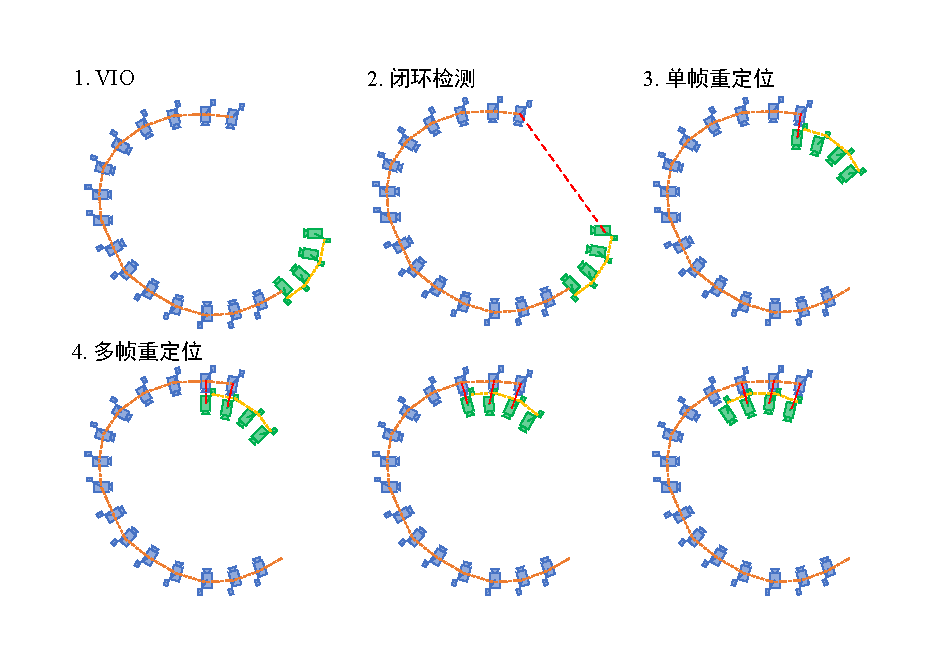
\includegraphics[width=0.4\textwidth, angle=-90]{figures/chapter4/fig4_8}
	\caption{重定位过程示意图}\label{fig4_8}
\end{figure}
\subsection{闭环优化}
之前讨论的BA优化,往往是同时优化位姿及其3D路标点,这样会存在一个问题:随着时间的累计,相机的运动距离越来越远,路标点也在不断增加,如果不使用滑窗优化,而是优化过去所有的位姿和路标点,那么计算量会逐渐增加,计算效率会逐渐下降。当然,本系统中使用了滑窗策略,避免了这种情况。但是,为了达到全局一致性的目的,当检测到闭环的时候,希望进行一次全局优化。为了避免极低的计算效率,采用位姿图优化,而不是全局BA优化。位姿图优化,顾名思义,只对位姿进行优化,而忽略路标点。这样做的原因是,通常路标点经过多次观测优化后会收敛到一个固定值,而那些发散的异常点会消失不见。对于那些收敛的点,不需一直进行优化。在闭环之前,路标点肯定都经过了多次优化,已经收敛,所以闭环的时候没有必要再次优化,而只需要优化位姿即可。

图优化是由节点和边构成的,节点是待优化的变量,边是约束关系。那么位姿图呢?位姿图的节点表示相机位姿,用李代数 $ \bm{ \xi}_{1}, {\ldots}, \bm{\xi}_{n} $ 表示,位姿图的边是位姿间相机的运动,用 $\Delta \boldsymbol{\xi}_{i j} $ 表示位姿 $\bm{\xi}_{i} $和$\bm{\xi}_{i} $ 之间的相机运动,则,
\begin{equation}
\label{eqn:4.35}
\setlength{\abovedisplayskip}{6pt}
\setlength{\belowdisplayskip}{6pt}
\Delta \boldsymbol{\xi}_{i j}=\boldsymbol{\xi}_{i}^{-1} \circ \boldsymbol{\xi}_{j}=\ln \left(\exp \left(\left[-\boldsymbol{\xi}_{i}\right]_\times \right) \exp \left(\left[\boldsymbol{\xi}_{j}\right]_\times\right)\right)^{\vee}
\end{equation}
或者可以用李群表示为:
\begin{equation}
\label{eqn:4.36}
\setlength{\abovedisplayskip}{6pt}
\setlength{\belowdisplayskip}{6pt}
\Delta \boldsymbol{T}_{i j}=\boldsymbol{T}_{i}^{-1} \boldsymbol{T}_{j}
\end{equation}
上式中的“=”不完全成立,将利用这个误差来构建残差项:
\begin{equation}
\label{eqn:4.37}
\setlength{\abovedisplayskip}{6pt}
\setlength{\belowdisplayskip}{6pt}
\begin{aligned} 
	\boldsymbol{e}_{i j} &=\ln \left(\Delta \boldsymbol{T}_{i j}^{-1} \boldsymbol{T}_{i}^{-1} \boldsymbol{T}_{j}\right)^{\vee} \\ 
	&=\ln \left( \exp \left(\left[-\boldsymbol{\xi}_{i j}\right]_\times \right) \exp \left(\left[-\boldsymbol{\xi}_{i}\right]_\times\right) \exp \left( \left[\boldsymbol{\xi}_{j}\right]_\times \right)\right)^{\vee} 
\end{aligned}
\end{equation}

按照前面研究优化的思路,需要求残差对优化变量的一阶导数,仍旧用扰动求导的方式:
\begin{equation}
\label{eqn:4.38}
\setlength{\abovedisplayskip}{6pt}
\setlength{\belowdisplayskip}{6pt}
\hat{\boldsymbol{e}}_{i j}=
\ln \left(\boldsymbol{T}_{i j}^{-1} \boldsymbol{T}_{i}^{-1} \exp \left(\left[-\boldsymbol{\delta} \boldsymbol{\xi}_{i}\right]_\times\right) 
\exp \left(\left[\delta \boldsymbol{\xi}_{j}\right]_\times\right) \boldsymbol{T}_{j}\right)^{\vee}
\end{equation}
其中, $\delta \bm{\xi}_{i} $和 $\delta \bm{\xi}_{j} $为 $\bm{\xi}_{i}  $和 $\bm{\xi}_{j}  $的左扰动。根据李群上的伴随性质,即
\begin{equation}
\label{eqn:4.39}
\setlength{\abovedisplayskip}{6pt}
\setlength{\belowdisplayskip}{6pt}
\exp \left(\left[\operatorname{Ad}(\boldsymbol{T}) \boldsymbol{\xi}\right]_\times\right)=
\boldsymbol{T} \exp \left( \left[\boldsymbol{\xi}\right]_\times\right) \boldsymbol{T}^{-1}
\end{equation}
其中,
\[\operatorname{Ad}(\boldsymbol{T})=\left[ \begin{array}{cc}{\boldsymbol{R}} & {\left[\boldsymbol{t}\right]_\times \boldsymbol{R}} \\ {0} & {\boldsymbol{R}}\end{array}\right]\]
可得,
\begin{equation}
\label{eqn:4.40}
\exp \left( \left[\boldsymbol{\xi}\right]_\times\right) \boldsymbol{T}=
\boldsymbol{T} \exp \left(\left[\operatorname{Ad}\left(\boldsymbol{T}^{-1}\right) \boldsymbol{\xi}\right]_\times\right)
\end{equation}
利用式(\ref{eqn:4.40}),将扰动移到最右侧,从而推导出右乘雅可比矩阵:
\begin{equation}
\label{eqn:4.41}
\begin{aligned} 
\hat{\bm{e}}_{i j} &=
\ln \left\{
\boldsymbol{T}_{i j}^{-1} \boldsymbol{T}_{i}^{-1} 
\exp \left( \left[-\delta \boldsymbol{\xi}_{i}\right]_\times \right) 
\exp \left( \left[\delta \boldsymbol{\xi}_{j}\right]_\times \right) \boldsymbol{T}_{j}
\right\}^{\vee} \\
&=
\ln \left\{
\boldsymbol{T}_{i j}^{-1} \boldsymbol{T}_{i}^{-1} \boldsymbol{T}_{j} 
\exp \left(
\left[-\mathrm{Ad}\left(\boldsymbol{T}_{j}^{-1}\right) \boldsymbol{\delta} \boldsymbol{\xi}_{i}\right]_\times
\right) 
\exp \left(
\left[\mathrm{A} \mathrm{d}\left(\boldsymbol{T}_{j}^{-1}\right) \boldsymbol{\delta} \boldsymbol{\xi}_{j}\right]_\times
\right)
\right\} ^ {\vee}\\
& \approx \boldsymbol{e}_{i j} + \frac{\partial \boldsymbol{e}_{i j}}{\partial \delta \xi_{i}} \boldsymbol{\delta} \boldsymbol{\xi}_{i} 
+ \frac{\partial \boldsymbol{e}_{i j}}{\partial \delta \xi_{j}} \boldsymbol{\delta} \boldsymbol{\xi}_{j}
\end{aligned}
\end{equation}
其中,
\begin{equation}
\label{eqn:4.42}
\begin{aligned}
\frac{\partial \boldsymbol{e}_{i j}}{\partial \delta \xi_{i}} &= -\bm{\mathcal{J}}_{r}^{-1}\left(\boldsymbol{e}_{i j}\right) \operatorname{Ad}\left(\boldsymbol{T}_{j}^{-1}\right) \\
\frac{\partial \boldsymbol{e}_{i j}}{\partial \boldsymbol{\delta} \xi_{j}} &= \bm{\mathcal{J}}_{r}^{-1}\left(\boldsymbol{e}_{i j}\right) \operatorname{Ad}\left(\boldsymbol{T}_{j}^{-1}\right)
\end{aligned}
\end{equation}
一般李代数上的雅可比矩阵比较复杂,通常近似取为:
\begin{equation}
\label{eqn:4.43}
\bm{\mathcal{J}}_{r}^{-1}\left(\boldsymbol{e}_{i j}\right) \approx 
\boldsymbol{I}+\frac{1}{2} \left[ 
\begin{array}{cc}
{\left[\boldsymbol{\phi}_{\boldsymbol{e}} \right]_\times} & { \left[ \boldsymbol{\rho}_{\boldsymbol{e}} \right]_\times } \\ 
{\mathbf{0}} & { \left[\bm{\phi}_{\boldsymbol{e}}\right]_\times}
\end{array}
\right]
\end{equation}
到此为止,求的仅仅是位姿图中的一条边的残差,记所有边的集合为 ,那么所有边的残差就构成了目标函数:
\begin{equation}
\label{eqn:4.44}
\min _{\bm{\xi}} \frac{1}{2} \sum_{i, j \in \mathcal{E}} \bm{e}_{i j}^{T} \Sigma_{i j}^{-1} \bm{e}_{i j}
\end{equation}
然后用高斯-牛顿或者LM方法迭代求解最优值。

在本系统中,当检测到闭环的时候,进行全局位姿优化。这里的位姿指3自由度位置 $(x,y,z) $和一个偏航角 $\hat{\psi}_{ij} $,总共四自由度。忽略横滚角和俯仰角是因为在单目/视觉惯性融合系统中,这两个角度是可以根据重力的方向观测到的,不会产生累计漂移。

当滑动窗口中最旧的那一帧关键帧滑出窗口时,它将被添加到位姿图中。该关键帧是位姿图的顶点,它通过两条边和其他顶点相连:

(1)第一条边是滑动窗口中的两个关键帧之间的相对变换(或者叫相对位姿),称为序列边。假设关键帧 $i$ 是最新进行边缘化的帧,其之前的某一个关键帧为 $j$ ,那么序列边为包括 $i$ 和 $j$ 的相对位移 $\hat{\mathbf{p}}_{ij}^i $ 以及偏航角 $\hat{\psi}_{ij} $ :
\begin{equation}
\label{eqn:4.45}
\setlength{\abovedisplayskip}{6pt}
\setlength{\belowdisplayskip}{6pt}
\begin{split}
\hat{\mathbf{p}}_{ij}^i&=\hat{\mathbf{R}}_i^{w^{-1}}(\hat{\mathbf{p}}_j^w-\hat{\mathbf{p}}_i^w) \\
\hat{\psi}_{ij}&=\hat{\psi}_j-\hat{\psi}_i.
\end{split}
\end{equation}

(2)第二条边是检测到闭环后形成的闭环边。其定义和式(\ref{eqn:4.45})一样,通过重定位获得闭环边的值。

有了顶点和边,就可以得到图优化的残差项及目标函数。定义关键帧 $i$ 和 $j$ 之间的残差为:
\begin{equation}
\label{eqn:4.46}
\mathbf{r}_{i,j}(\mathbf{p}_i^w,\psi_i,\mathbf{p}_j^w,\psi_j)=\begin{bmatrix}
\mathbf{R}(\hat{\phi}_i,\hat{\theta}_i,\psi_i)^{-1}(\mathbf{p}_j^w-\mathbf{P}_i^w)-\hat{\mathbf{p}}_{ij}^i \\
\psi_j-\psi_i-\hat{\psi}_{ij}
\end{bmatrix}
\end{equation}
其中,$\hat{\phi}_i,\hat{\theta}_i $ 是单目VIO估计出的横滚角和俯仰角。

所有的序列边和闭环边的残差项之和构成了整体的目标函数:
\begin{equation}
\label{eqn:4.47}
\begin{split}
\underset{\mathcal{\mathbf{p},\psi}}{\text{min}}
\left\{
\sum_{(i,j)\in\mathcal{S}}\left\| \mathbf{r}_{i,j} \right\|^2+\sum_{(i,j)\in\mathcal{L}}\rho(\left\| \mathbf{r}_{i,j} \right\|^2)
\right\}
\end{split}
\end{equation}
其中 $\mathcal{S} $ 是所有序列边的集合,$\mathcal{L} $ 是所有闭环边的集合。$\rho(\cdot) $  是Huber范数。对闭环边使用Huber范数是为了减少错误闭环的影响,而对于序列边不使用Huber范数,因为序列边是VIO给出的,VIO已经经行了“异常点”剔除。

位姿图优化和重新定位将异步运行在两个独立的线程中,以便在进行重定位时,能立即使用最优化的位姿图。同样,即使当前的姿态图优化尚未完成,仍然可以使用现有的姿态图进行重定位。这一过程如图\ref{fig4_9}所示。
\begin{figure}[h]\setlength{\belowcaptionskip}{-12pt}
	\centering
	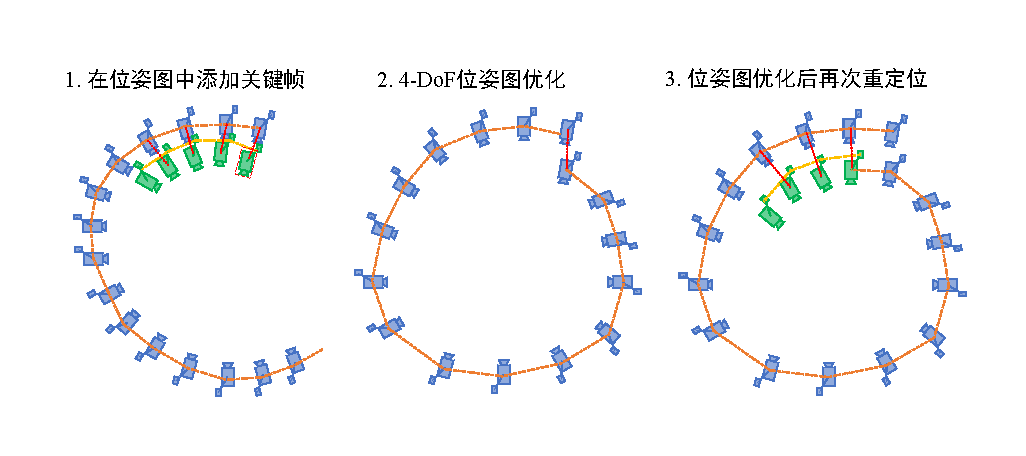
\includegraphics[width=0.3\textwidth, angle=-90]{figures/chapter4/fig4_9}
	\caption{位姿优化示意图}\label{fig4_9}
\end{figure}
\section{本章小结}
本章对系统的后端优化和闭环检测算法进行了详细的阐述。首先研究了后端优化的优化变量、目标函数以及构成目标函数的各个残差项,并解释了边缘化过程。然后研究了基于词袋模型的闭环检测算法。最后分析了重定位的实现过程,以及基于图优化的闭环优化算法。本章研究的优化算法体现了视觉和IMU之间的紧耦合过程,二者的状态量放在一起进行优化,紧密结合,相辅相成。
\chapter{实验}
\label{chap:5}
在本章中,主要研究实验方案,以及分析实验结果。首先使用公开数据集EuRoc进行实验验证,EuRoc是室内飞行数据集,提供6-DoF真值。然后使用本系统进行在线实时验证,本系统放在车顶,围绕北京理工大学中关村校区进行车载实验验证。EuRoc数据集是室内环境,飞行路程短,包含6-DoF位姿真值。本地实验是室外环境,汽车行程远,包含2-DoF位置真值。
\section{EuRoc数据集实验}
\subsection{EuRoc构成及硬件平台}
EuRoc飞行数据集是苏黎世联邦理工学院自动系统实验室于2016年发布的公开数据集\upcite{burri2016euroc},主要用于视觉SLAM和视觉/惯性融合的研究上。数据集中包含如下可用数据:\\
(1)视觉/惯性数据
\vspace{-0.26cm}
\begin{itemize}
	\setlength{\itemsep}{-5pt}
	\item 双目图像。使用Aptina MT9V034全局快门相机拍摄,单色图像,帧率为20FPS;
	\item IMU数据。使用ADIS16448测量角速率和加速度,采集频率为200 Hz;
	\item 对齐的时间戳。
\end{itemize}
\vspace{-0.26cm}
(2)地面真值数据
\vspace{-0.26cm}
\begin{itemize}
	\setlength{\itemsep}{-5pt }
	\item 6-DoF位姿真值。通过Vicon系统得到;
	\item 3-DoF位置真值。通过Leica MS50激光跟踪仪测量得到;
	\item 3D空间结构。通过徕卡MS50 3D结构扫描仪器扫描得到。
\end{itemize}
\vspace{-0.26cm}
(3)标定数据
\vspace{-0.26cm}
\begin{itemize}
	\setlength{\itemsep}{-5pt }
	\item 相机内参;
	\item 相机-IMU外参;
	\item 时空对齐的地面真值。
\end{itemize}
\vspace{-0.26cm}

如图\ref{fig5_1}所示是EuRoc的硬件平台。图\ref{fig5_1}(a)是无人机,图\ref{fig5_1}(b)是无人机上搭载的视觉/惯性传感器。

使用EuRoc数据集中的MH\_01\_easy和MH\_05\_difficult两组数据,这两组数据是在机器大厅采集的,代表了“容易”和“困难”两种环境。图\ref{fig5_2}(a)是机器大厅环境图,图\ref{fig5_2}(b)是传感器和地面真值测量仪器之间的位置示意图。
\begin{figure}[h]\setlength{\belowcaptionskip}{-12pt}
	\centering
	\subfigure[]{
		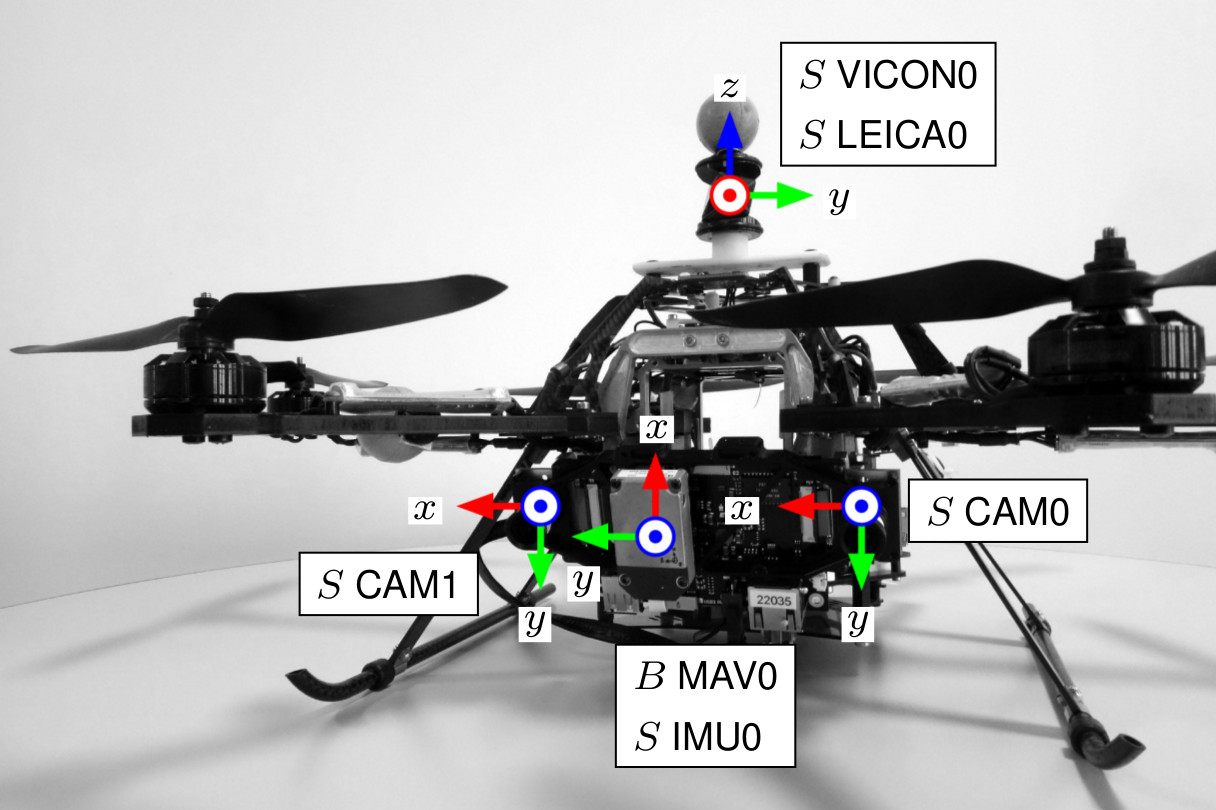
\includegraphics [width=0.35\textwidth]{figures/chapter5/fig5_1_1}}
	\hspace{0.5cm}
	\subfigure[]{
		\includegraphics [width=0.35\textwidth]{figures/chapter5/fig5_1_2}}
	\caption{EuRoc硬件平台} \label{fig5_1}
\end{figure}

\begin{figure}[h]\setlength{\belowcaptionskip}{-12pt}
	\centering
	\subfigure[]{
	\includegraphics [width=0.42\textwidth]{figures/chapter5/fig5_2_1}}
	\hspace{0.5cm}
	\subfigure[]{
	\includegraphics [width=0.35\textwidth]{figures/chapter5/fig5_2_2}}
	\caption{(a)机器大厅环境;(b)传感器和地面真值测量仪器之间的位置示意图} \label{fig5_2}
\end{figure}
\subsection{EuRoc实验一}
首先使用MH\_01\_easy进行实验。图\ref{fig5_3}是三维定位轨迹图对比图,图\ref{fig5_4}是三轴位置(x, y, z)对比图,图\ref{fig5_5}是三轴姿态(roll, pitch, yaw)对比图。其中VI\_SLAM是本系统输出轨迹,GroundTruth是数据集中的真值轨迹。通过图\ref{fig5_3},图\ref{fig5_4}和图\ref{fig5_5},可以定性分析系统的定位误差。
\begin{figure}
	\centering
	\includegraphics[width=0.7\textwidth]{figures/chapter5/traject_mh01}
	\caption{EuRoc实验一的三维定位轨迹图}\label{fig5_3}
\end{figure}
\begin{figure}
	\centering
	\includegraphics[width=1.0\textwidth]{figures/chapter5/xyz_mh01}
	\caption{EuRoc实验一的三轴位置(x, y, z)对比图}\label{fig5_4}
\end{figure}
\begin{figure}[!h]
	\centering
	\includegraphics[width=1.0\textwidth]{figures/chapter5/rpy_mh01}
	\caption{EuRoc实验一的三轴姿态(roll, pitch, yaw)对比图}\label{fig5_5}
\end{figure}

然后定量分析EuRoc实验一中系统的定位误差。图\ref{fig5_6}是三维定位绝对误差图。计算出系统定位的绝对误差(APE),均方根误差(RMSE),标准差(STD),平均误差(MEAN)和中值误差(MEDIAN),将计算结果展示在表\ref{tab:5.1}中。为了更加直观,将这些误差以曲线图的形式展示出来,如图\ref{fig5_7}所示。
\begin{figure}[!h]
	\centering
	\includegraphics[width=0.7\textwidth]{figures/chapter5/ape_map_mh01}
	\caption{EuRoc实验一的三维定位绝对误差图}\label{fig5_6}
\end{figure}
\begin{figure}
	\centering
	\includegraphics[width=1.0\textwidth]{figures/chapter5/ape_err_mh01}
	\caption{EuRoc实验一的系统定位误差指标图}\label{fig5_7}
\end{figure}
\begin{table}[!h]
	\zihao{5}
	\centering
	\caption{EuRoc实验一的系统定位误差指标} \label{tab:5.1}
	\begin{tabular*}{0.9\textwidth}{@{\extracolsep{\fill}}cccccc}
		\toprule
		APE\_MAX(m)&APE\_MIN(m) &RMSE	&STD	&MEAN(m)	&MEDIAN(m) \\
		\midrule
		0.6403	&0.0447	&0.2820	&0.1212	&0.2546	&0.2199\\
		\bottomrule
	\end{tabular*}
\end{table}

对比其他开源VIO方案在MH\_01\_easy上的误差的RMSE\upcite{delmerico2018benchmark},MSCKF为0.43,OKVIS为0.16,ROVIO为0.21,可见本系统在MH\_01\_easy上的定位精度介于MSCKF和ROVIO之间。
\subsection{EuRoc实验二}
使用MH\_05\_difficult数据集进行实验。图\ref{fig5_8}是三维定位轨迹图对比图,图\ref{fig5_9}是三轴位置(x, y, z)对比图,图\ref{fig5_10}是三轴姿态(roll, pitch, yaw)对比图。其中VI\_SLAM是本系统输出轨迹,GroundTruth是数据集中的真值轨迹。通过图\ref{fig5_8},图\ref{fig5_9}和图\ref{fig5_10},可以定性分析系统的定位误差。
\begin{figure}
	\centering
	\includegraphics[width=0.7\textwidth]{figures/chapter5/traject_mh05}
	\caption{EuRoc实验二的三维定位轨迹图}\label{fig5_8}
\end{figure}
\begin{figure}
	\centering
	\includegraphics[width=1.0\textwidth]{figures/chapter5/xyz_mh05}
	\caption{EuRoc实验二的三轴位置(x, y, z)对比图}\label{fig5_9}
\end{figure}
\begin{figure}[!h]
	\centering
	\includegraphics[width=1.0\textwidth]{figures/chapter5/rpy_mh05}
	\caption{EuRoc实验二的三轴姿态(roll, pitch, yaw)对比图}\label{fig5_10}
\end{figure}

然后定量分析EuRoc实验二中系统的定位误差。图\ref{fig5_11}是三维定位绝对误差图。同样,计算出APE,RMSE,STD,MEAN和MEDIAN,将计算结果展示在表\ref{tab:5.2}中。为了更加直观,将这些误差以曲线图的形式展示出来,如图\ref{fig5_12}所示。\newpage
\begin{figure}[!h]\setlength{\belowcaptionskip}{-12pt}
	\centering
	\includegraphics[width=0.75\textwidth]{figures/chapter5/ape_map_mh05}
	\caption{EuRoc实验二的三维定位绝对误差图}\label{fig5_11}
\end{figure}
\begin{figure}[!h]\setlength{\belowcaptionskip}{-12pt}
	\centering
	\includegraphics[width=1.0\textwidth]{figures/chapter5/ape_err_mh05}
	\caption{EuRoc实验二的系统定位误差指标图}\label{fig5_12}
\end{figure}
\begin{table}[!h]\setlength{\abovecaptionskip}{6pt}
	\zihao{5}
	\centering
	\caption{EuRoc实验二的系统定位误差指标} \label{tab:5.2}
	\begin{tabular*}{0.9\textwidth}{@{\extracolsep{\fill}}cccccc}
		\toprule
		APE\_MAX(m)&APE\_MIN(m) &RMSE	&STD	&MEAN(m)	&MEDIAN(m) \\
		\midrule
		0.4739	&0.0134	&0.1999	&0.0901	&0.1784	&0.1616\\
		\bottomrule
	\end{tabular*}
\end{table}

对比其他开源VIO方案在MH\_05\_difficult上的误差的RMSE\upcite{delmerico2018benchmark},MSCKF为0.48,OKVIS为0.56,ROVIO为0.52,可见本系统在MH\_01\_difficult上的定位精度要远远高于其他开源方案。这也说明了本系统更加适应复杂环境,鲁棒性更高。
\section{本地实时实验}
\subsection{本地实验硬件及环境}
使用实验室的丰田SUV进行车载实验,如图\ref{fig5_13}(a)所示。图\ref{fig5_13}(b)是搭载在车顶上的多传感器硬件系统,其具体构成已经在2.3.1小节中介绍。
\begin{figure}[h]\setlength{\belowcaptionskip}{-12pt}
	\centering
	\subfigure[]{
	\includegraphics [width=0.3\textwidth]{figures/chapter5/fig5_13_1}}
	\hspace{0.5cm}
	\subfigure[]{
	\includegraphics [width=0.25\textwidth]{figures/chapter5/fig5_13_2}}
	\caption{本地实验设备} \label{fig5_13}
\end{figure}

本地车载实验的路线有两个,一个是环绕半个北京理工大学中关村校区,大约2.8km,如图\ref{fig5_14}黄色GPS轨迹线所示。另一个是环绕整个北京理工大学中关村校区一周,大约4.3km,如图\ref{fig5_14}红色GPS轨迹线所示。
\begin{figure}[h]\setlength{\belowcaptionskip}{-12pt}
	\centering
	\includegraphics[width=0.45\textwidth]{figures/chapter5/fig5_14}
	\caption{车载实验路线}\label{fig5_14}
\end{figure}
由于是车载实验,所以本系统只关注2自由度(x,y)位置,忽略高度。本系统使用RTK采集经纬度信息,经过高斯投影后转化为WGS-84坐标,用这个坐标点轨迹作为真值数据。所以,本系统的真值数据也只有2自由度位置信息,没有姿态真值。
\subsection{本地实验一}
实验一的行车轨迹如图\ref{fig5_14}黄线所示。图\ref{fig5_15}是二维定位轨迹图对比图,图\ref{fig5_16}是二轴位置(x, y)对比图。其中VI\_SLAM是本系统输出轨迹,RTK是差分GPS轨迹。通过图\ref{fig5_15}和图\ref{fig5_16},可以定性分析系统的定位误差。
\begin{figure}[h]\setlength{\belowcaptionskip}{-12pt}
	\centering
	\includegraphics[width=0.90\textwidth]{figures/chapter5/traject_3km}
	\caption{本地实验一的二维定位轨迹图对比图}\label{fig5_15}
\end{figure}
\begin{figure}[h]\setlength{\belowcaptionskip}{-12pt}
	\centering
	\includegraphics[width=1.0\textwidth]{figures/chapter5/xy_3km}
	\caption{本地实验一的二轴位置(x, y)对比图}\label{fig5_16}
\end{figure} 

然后定量分析本地实验一中系统的定位误差。图\ref{fig5_17}是二维定位绝对误差图。同样,计算出APE,RMSE,STD,MEAN和MEDIAN,将计算结果展示在表\ref{tab:5.3}中。为了更加直观,将这些误差以曲线图的形式展示出来,如图\ref{fig5_18}所示。\newpage
\begin{figure}[!h]\setlength{\belowcaptionskip}{-12pt}
	\centering
	\includegraphics[width=0.90\textwidth]{figures/chapter5/ape_map_3km}
	\caption{本地实验一的二维定位绝对误差图}\label{fig5_17}
\end{figure}\newpage
\begin{figure}[!h]\setlength{\belowcaptionskip}{-12pt}
	\centering
	\includegraphics[width=1.0\textwidth]{figures/chapter5/ape_err_3km}
	\caption{本地实验一的系统定位误差指标图}\label{fig5_18}
\end{figure}
\begin{table}[!h]\setlength{\abovecaptionskip}{6pt}
	\zihao{5}
	\centering
	\caption{本地实验一的系统定位误差指标} \label{tab:5.3}
	\begin{tabular*}{0.9\textwidth}{@{\extracolsep{\fill}}cccccc}
		\toprule
		APE\_MAX(m)&APE\_MIN(m) &RMSE	&STD	&MEAN(m)	&MEDIAN(m) \\
		\midrule
		19.5912	 &5.9771	&13.0965	&2.5359	 &12.8487	&12.6319 \\
		\bottomrule
	\end{tabular*}
\end{table}

可见,本地实验一的最大定位误差是19.5912米,定位精度≤0.6\%。\newpage
\subsection{本地实验二}
实验二的行车轨迹如图\ref{fig5_14}红线所示。图\ref{fig5_19}是二维定位轨迹图对比图,图\ref{fig5_20}是二轴位置(x, y)对比图。其中VI\_SLAM是本系统输出轨迹,RTK是差分GPS轨迹。通过图\ref{fig5_19}和图\ref{fig5_20},可以定性分析系统的定位误差。
\begin{figure}[h]\setlength{\belowcaptionskip}{-12pt}
	\centering
	\includegraphics[width=0.90\textwidth]{figures/chapter5/traject_5km}
	\caption{本地实验二的二维定位轨迹图对比图}\label{fig5_19}
\end{figure}
\begin{figure}[h]\setlength{\belowcaptionskip}{-12pt}
	\centering
	\includegraphics[width=1.0\textwidth]{figures/chapter5/xy_5km}
	\caption{本地实验二的二维位置(x, y)对比图}\label{fig5_20}
\end{figure}

然后定量分析本地实验二中系统的定位误差。图\ref{fig5_21}是二维定位绝对误差图。同样,计算出APE,RMSE,STD,MEAN和MEDIAN,将计算结果展示在表\ref{tab:5.4}中。为了更加直观,将这些误差以曲线图的形式展示出来,如图\ref{fig5_22}所示。\newpage
\begin{figure}[!h]
	\centering
	\includegraphics[width=0.90\textwidth]{figures/chapter5/ape_map_5km}
	\caption{本地实验二的二维定位绝对误差图}\label{fig5_21}
\end{figure}
\begin{figure}[!h]\setlength{\belowcaptionskip}{-12pt}
	\centering
	\includegraphics[width=0.85\textwidth]{figures/chapter5/ape_err_5km}
	\caption{本地实验二的系统定位误差指标图}\label{fig5_22}
\end{figure}
\begin{table}[!h]\setlength{\abovecaptionskip}{6pt}
	\zihao{5}
	\centering
	\caption{本地实验二的系统定位误差指标} \label{tab:5.4}
	\begin{tabular*}{0.9\textwidth}{@{\extracolsep{\fill}}cccccc}
		\toprule
		APE\_MAX(m)&APE\_MIN(m) &RMSE	&STD	&MEAN(m)	&MEDIAN(m) \\
		\midrule
		56.6838	&3.2654	&27.9445	&14.3974	&23.9501	&18.2750 \\
		\bottomrule
	\end{tabular*}
\end{table}

可见,本地实验二的最大定位误差是56.6838米,定位精度≤1.3\%。相比于本地实验一,定位精度有所下降。
\section{本章小结}
本章通过实验验证了本系统的定位效果。首先使用EuRoc数据集,验证了本系统在三维空间中的定位效果。然后进行本地校园车载实验,验证了本系统在大地平面上的定位效果。其中,EuRoc是室内环境,飞行距离短,环境简单。校园车载实验是室外环境,行驶路线长,环境复杂多变。两种环境下的实验数据说明本系统在不同的环境下都能正常工作,在短距离情况下定位精度较高,但是随着距离的增加,绝对定位精度会逐渐下降。
%%==================================================
%% conclusion.tex for BIT Master Thesis
%% modified by yang yating
%% version: 0.1
%% last update: Dec 25th, 2016
%%==================================================


\begin{conclusion}
如今,飞速发展人工智能(AI)正在各个领域展露锋芒,AI工作者期望利用AI改善人类生活。移动机器人、无人车和无人机等领域也属于人工智能的一部分。无人载体要实现无人驾驶的目标,通常需要具有自主定位、地图构建、目标识别、智能避障和路径规划等功能。单一传感器不能完成所有的这些功能,所以无人设备上往往搭载多种传感器,以便弥补单一传感器的不足之处。其中,Visual和IMU一般情况下是无人载体上的必备传感器。Visual和IMU在功能上有很多的互补性,将二者融合能够获得高精度的位姿估计。本文正是以视觉和IMU为对象,总结国内外视觉SLAM以及VIO的研究现状,深入研究Visual-IMU的融合算法,同时搭建硬件设备,将硬件设备和软件算法结合起来构建一套多传感融合定位系统。

本文首先详细研究了传感器的数学模型,以及如何选择相机和IMU。然后对相机和IMU的标定原理和方法进行了分析总结,并给出了标定结果。同时研究了硬件同步的方法。之后研究了基于ROS的传感器信息采集方法。然后进入算法部分,首先研究前端算法,包括图像特征的提取与跟踪,特征的异常点剔除方法,IMU预积分理论。然后研究初始化算法,包括对极几何、三角测量、PnP等理论基础,纯视觉初始化流程,以及视觉/IMU联合初始化方法。前端和初始化为后端非线性优化提供初始值,是后端优化的基础。

本文的后续部分对后端优化和闭环进行了深入研究。首先研究了紧耦合非线性滑窗优化方法,定义了优化的状态量以及目标函数,并对各个残差项进行详细的分析。接着为了使滑窗策略不丢失历史信息,研究了边缘化理论,并研究了本系统的边缘化方法。然后本文研究了闭环检测算法,对词袋模型和字典构建进行了细致的研究。最后,针对检测到的闭环帧,研究了如何对闭环帧进行重定位,如何在检测到闭环后对所有的关键帧进行位姿优化,获得全局一致的定位轨迹。

在文章的最后,针对本系统做了两组实验。一组是公开数据集EuRoc实验,另一组是本地校园车载实时实验。实验环境从简单到复杂,从短距离到长距离。两组本地实验的定位精度分别为0.6\%和1.3\%,表明了本系统的可靠性和有效性。

然而本系统仍旧有一些不足之处,故提出以下需要改进的地方:

1.在硬件方面,本系统的硬件同步做的还不完善,目前IMU和相机同步的时间差在毫秒级,而数据集可以达到微秒级。原因在于本系统的硬件同步电路仅仅采用了一片CD4017计数器,没有添加复杂的滤波电路,可能导致触发脉冲的精度不够高和响应时间不够短。

2. 算法方面,本系统算法复杂,代码繁多,计算量大,目前只能在Intel NUC或者个人PC上进行计算,无法移植到小型的嵌入式设备。后续研究需要对算法和代码进行优化,降低整体计算量。

3. 对于磁力计,鉴于磁力计容易受外界环境干扰,测量数据不稳定,外参标定复杂的情况,本系统仅仅使用磁力计进行航向初始化,并未在后端优化中使用。后续将研究如何对磁力计进行动态补偿、滤波,以获得稳定可用的数据,并将其融合在后端优化中。
\end{conclusion}

%% 参考文献,五号字,使用 BibTeX,包含参考文献文件.bib

%\bibliography{reference/chap1,reference/chap2} %多个章节的参考文献
\bibliography{reference/chap1}


%%%%%%%%%%%%%%%%%%%%%%%%%%%%%%
%% 后置部分
%%%%%%%%%%%%%%%%%%%%%%%%%%%%%%

%% 附录(章节编号重新计算,使用字母进行编号)
%\appendix
%\renewcommand\theequation{\Alph{chapter}--\arabic{equation}}  % 附录中编号形式是"A-1"的样子
%\renewcommand\thefigure{\Alph{chapter}--\arabic{figure}}
%\renewcommand\thetable{\Alph{chapter}--\arabic{table}}

%%%==================================================
%% app1.tex for BIT Master Thesis
%% modified by yang yating
%% version: 0.1
%% last update: Dec 25th, 2016
%%==================================================


\chapter{***}

附录相关内容…
 
%
\chapter{Maxwell Equations}


因为在柱坐标系下,$\overline{\overline\mu}$是对角的,所以Maxwell方程组中电场$\bf
E$的旋度

所以$\bf H$的各个分量可以写为:
\begin{subequations}
  \begin{eqnarray}
    H_r=\frac{1}{\mathbf{i}\omega\mu_r}\frac{1}{r}\frac{\partial
      E_z}{\partial\theta } \\
    H_\theta=-\frac{1}{\mathbf{i}\omega\mu_\theta}\frac{\partial E_z}{\partial r}
  \end{eqnarray}
\end{subequations}
同样地,在柱坐标系下,$\overline{\overline\epsilon}$是对角的,所以Maxwell方程组中磁场$\bf
H$的旋度
\begin{subequations}
  \begin{eqnarray}
    &&\nabla\times{\bf H}=-\mathbf{i}\omega{\bf D}\\
    &&\left[\frac{1}{r}\frac{\partial}{\partial
        r}(rH_\theta)-\frac{1}{r}\frac{\partial
        H_r}{\partial\theta}\right]{\hat{\bf
        z}}=-\mathbf{i}\omega{\overline{\overline\epsilon}}{\bf
      E}=-\mathbf{i}\omega\epsilon_zE_z{\hat{\bf z}} \\
    &&\frac{1}{r}\frac{\partial}{\partial
      r}(rH_\theta)-\frac{1}{r}\frac{\partial
      H_r}{\partial\theta}=-\mathbf{i}\omega\epsilon_zE_z
  \end{eqnarray}
\end{subequations}
由此我们可以得到关于$E_z$的波函数方程:
\begin{eqnarray}
  \frac{1}{\mu_\theta\epsilon_z}\frac{1}{r}\frac{\partial}{\partial r}
  \left(r\frac{\partial E_z}{\partial r}\right)+
  \frac{1}{\mu_r\epsilon_z}\frac{1}{r^2}\frac{\partial^2E_z}{\partial\theta^2}
  +\omega^2 E_z=0
\end{eqnarray}
 

%(其后部分无编号)
\backmatter

% 发表文章目录
%%==================================================
%% pub.tex for BIT Master Thesis
%% modified by yang yating
%% version: 0.1
%% last update: Dec 25th, 2016
%%==================================================

\begin{publications}{99}

       
\end{publications}

% 致谢
%%%==================================================
%% thanks.tex for BIT Master Thesis
%% modified by yang yating
%% version: 0.1
%% last update: Dec 25th, 2016
%%==================================================

\begin{thanks}
	
时光就这样一点一点偷偷溜走,短暂的硕士生涯已到终点。回首这两年在北理工求学的时光,不禁感慨万千,感恩至极。

首先我要感谢北京理工大学,感谢她给予我更上一层楼的机会,让我学到更多的知识,见识了更多的大师,感受到了大学之“大”。如果让我在回到当初的考研时期,我仍然不后悔选择北理工。

其次,我要感谢我的导师李磊磊老师。李老师平时为人和善,关心学生,一开始就给我留下了深刻的映像。在学习方面,李老师给与了我细心的指导,为我点明了方向,经常在我百思不得其解的时候给我指点,让我醍醐灌顶,茅塞顿开。其他老师也对我帮助颇多,严肃认真的陈家斌老师经常在我们开组会的时候给我们的课题提出宝贵的意见;谢玲老师待人和蔼可亲,对我的生活困难提供了莫大的帮助;刘星桥老师知识渊博,经常在我实验遇到困难的时候帮我分析问题、解决问题;韩勇强老师年轻有为,像师兄一样指导我们的课题,让我倍感亲切;徐建华老师、梁俊宇老师、宋春雷老师以及张磊师傅在我的学习和课题中都给予莫大的帮助,对此我深表感激。

然后,在平时的学习生活中,实验室的师兄师姐给我提供了很多的帮助和指引。余欢博士虽然远在澳大利亚,但是每次对于我的提问都耐心解答,在此向余欢师兄表示深深的谢意,祝福他学有所成,早日回国。王旒军师兄是我的本科师兄,待我如亲兄弟,在我本科和硕士期间都给与了我很大的帮助,也正是因为他我才进入了导航、制导与控制实验室,在此我由衷的对他说声谢谢。还要感谢我的搭档王京哲同学,王同学思维敏捷、聪明伶俐,给我很大的帮助。

再者,我要感谢我的父母,感谢他们将我养大,培养成材,在今后的生活中我会孝顺他们,陪他们到老。感谢我的女朋友,感谢她的理解与支持,感谢她一直在我身后做我坚强的精神后盾。

最后,再次感谢所有关心和帮助过我的人,感谢导航、制导与控制实验室,感谢BIT。

\end{thanks}

% 作者简介(博士论文需要)
%%%==================================================
%% resume.tex for BIT Master Thesis
%% modified by yang yating
%% version: 0.1
%% last update: Dec 25th, 2016
%%==================================================

\begin{resume}

本人…。

\end{resume}



\end{document}
